\chapter{Gramática Emergente en Dinámica Cortical}

\label{ch:phonetics}




\iftoggle{DEBUG}{
\section{Introducción}

Dada la complejidad del lenguaje humano, se hace difícil entender cómo los infantes pueden descubrir su estructura interna para lograr comportamiento comunicativo significativo.
Independientemente de ello, los infantes alcanzan tal comportamiento exitosamente en los primeros años de vida \cite{Saffran12874}.
Algunas líneas de investigación destacan la importancia de la estructura estadística que subyace el lenguaje en general \cite{Romberg2010StatisticalLA, 10.1371/journal.pone.0177794}, mientras que otras muestran que infantes de 11 a 20 meses de edad pueden adquirir diferentes aspectos de las reglas gramaticales abstractas \cite{doi:10.1111/infa.12094, doi:10.1111/j.1467-8624.2012.01869.x}.

Muchos modelos psico-lingüísticos proponen que en el procesamiento oracional en línea, se integran diferentes tipos de restricciones de manera coherente y rápida determinando cómo las palabras son sintácticamente combinadas en oraciones gramaticales \cite{Gibson1998-GIBCOS}.
Se propone que restricciones cualitativamente distintas como las estructuras semánticas/conceptuales, fonológicas y sintácticas operan de manera conjunta en una unión referencial dentro del modelo discursivo \cite{Rego1993TheCB, 10.1371/journal.pone.0177794}.
En algunos modelos, ciertas operaciones de unificación durante la comprensión oracional se ejecutan en paralelo a niveles semántico, sintáctico y fonológico \cite{Hagoort2005OnBB}.
Durante el proceso de comprensión en línea, se procesan los items léxicos secuencialmente en el curso del tiempo de duración de la entrada.
Los marcos estructurales asociados con cada palabra son combinados por medio de un mecanismo de unificación incremental en el orden que la entrada impone.

En el presente trabajo introducimos un modelo computacional bio-inspirado en el cual se asocia cada palabra desde el léxico mental con un marco estructural.
Cada marco estructural consiste de la combinación de la \gls{ds} \cite{doi:10.1080/00437956.1954.11659520} y de
información de categorías gramaticales sintácticas gruesas de palabras--específicamente la categoría \emph{palabras de función}, la categoría de \emph{palabras de contenido} y desde esta última segregamos la categoría de \emph{verbo}.
Se ha mostrado que la información de categorías gruesas de palabras utilizadas en este trabajo emergen desde restricciones fonológicas en etapas tempranas de adquisición del lenguaje \cite{doi:10.1207/s15327078in1002_5,lohmann_phonological_2017}.
Un marco estructural utilizado en este método constituye un  entorno para un item léxico particular.
En este modelo, las estructuras constitutivas de la oración son establecidas por medio de una operación de unificación que consiste en vincular \gls{ds},
sintaxis gruesa sustentada fonológicamente y restricciones secuenciales correlacionándolas de manera repetitiva hasta que una mejora en el desempeño de clasificación de constituyentes gramaticales emerge espontáneamente.
Esta emergencia en el mejoramiento de la clasificación en información gramaticalmente relevante, se obtiene sin ningún tipo de guia en optimización más allá de la correlación de las diferentes restricciones durante la oración.

En psicolingüística se propone que solamente una configuración frasal se mantiene activa entre los candidatos de vinculaciones alternativas.
Tal mecanismo de selección sería logrado por medio de un proceso de inhibición lateral entre dos o más vínculos de unificación alternativos \cite{Hagoort2005OnBB}.
De la misma manera, en nuestro modelo computacional, la información proveniente desde las dendritas laterales y apicales restringen la activación masiva de unidades excitadas por dendritas aferentes \cite{10.1371/journal.pone.0217966}.
Las dendritas aferentes reciben restricciones de \glsfirst{ds} mientras que las dendritas apicales reciben restricciones sintácticas gruesas.

En relación a la emergencia de restricciones sintácticas gruesas, se ha mostrado que mecanismos de aprendizaje implícito sustentados fonológicamente sirven como precursores para el aprendizaje de gramática en infantes de 4 meses \cite{10.1371/journal.pone.0017920}, en tal sentido la fonología sirve para el reconocimiento y la representación de \emph{palabras de función} en infantes aprendiendo Inglés \cite{doi:10.1207/s15327078in1002_5}, y en el proceso de derivación de entre \emph{sustantivos} y \emph{verbos} en Inglés \cite{lohmann_phonological_2017}.
Las dendritas laterales, por otro lado, reciben información desde activaciones previas en el mismo parche cortical poniendo la red al corriente de la secuencia de constituyentes léxicos a lo largo de la oración (Fig. \ref{fig:EncoderConnections}).

\begin{figure}[ht!]
    \centering
    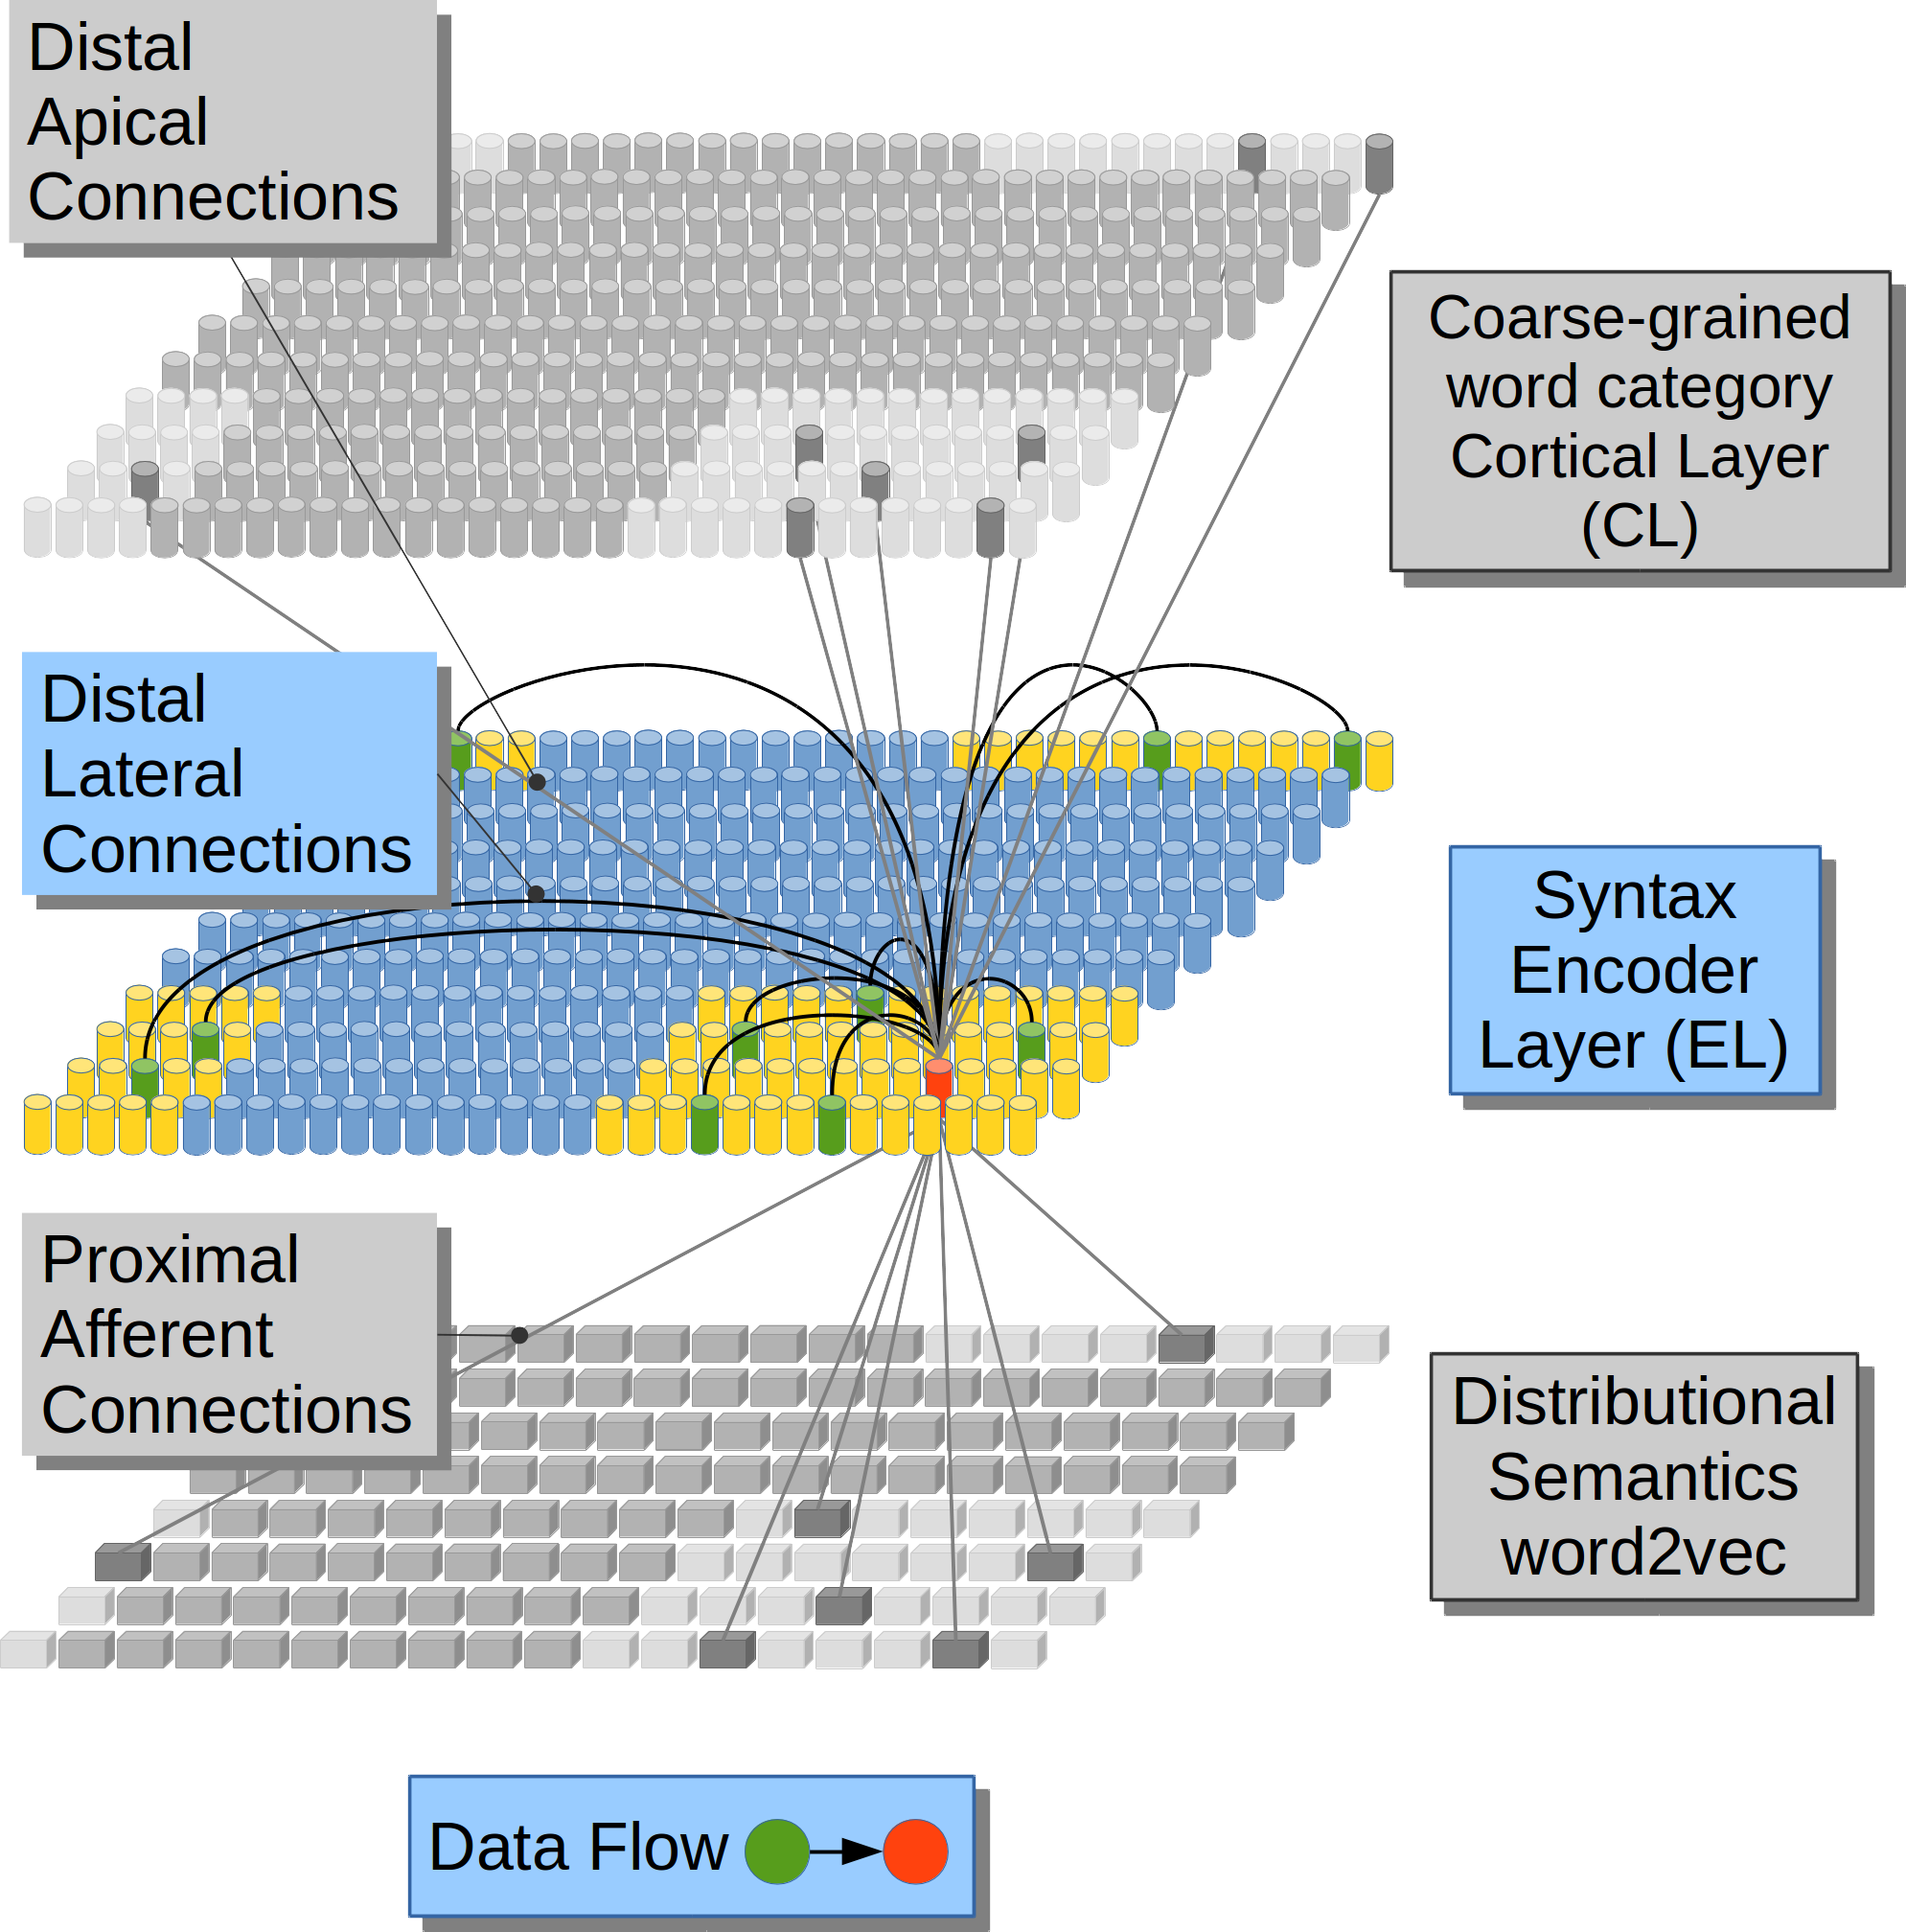
\includegraphics[width=0.6\textwidth]{EncoderConnections.png}
    \caption{Hipótesis Computacionales.
    Esquema de conexión para una \gls{cc} en la \gls{el}.
	    Cada cilindro en la \gls{el} y en la \gls{cl} representa una \gls{cc} en el tejido cortical.
	    Cada prisma en la Semántica Distributiva (word2vec) representa una variable de valor real.
	    Esta es una visualización de una \gls{cc} (en rojo) y de sus tres campos receptivos (lateral en amarillo y aferente y apical en gris claro).
    Esta es una figura adaptada de \url{https://doi.org/10.1371/journal.pone.0217966 bajo licencia CC-BY}.}
    \label{fig:EncoderConnections}
\end{figure}


En nuestro modelo computacional las restricciones de la \gls{ds} desde las dendritas aferentes excitan cúmulos de neuronas en la \glsfirst{el} en la Fig.~\ref{fig:EncoderConnections}.
La \gls{el} se podría referenciar a los parches corticales compuestos por el \glsfirst{ba} 45 y el \gls{ba} 44, las que se piensa contribuyen al procesamiento sintáctico \cite{Pallier2522, doi:10.1152/physrev.00006.2011, doi:10.1146/annurev-neuro-071013-013847}.
La \gls{el} recibe restricciones de \glsfirst{ds} en sus dendritas aferentes. Esta característica en la simulación toma en cuenta la información que viene desde las \gls{ba_pl} 47 y 45 las cuales están involucradas en el procesamiento semántico \cite{GOUCHA2015294, DECARLI2007933, PMID:15528098, NEWMAN201051}.
La información de la \gls{ds} tiende a activar cúmulos de unidades en la \gls{el}. Tales activaciones son masivas en principio, cubriendo todas las hipótesis léxicas traídas por la información de la \glsfirst{ds}. 
Todas las hipótesis léxicas activadas por las dendritas aferentes son atenuadas por las dendritas distales que reciben activaciones previas desde la misma \gls{el} (lateral) y por las dendritas distales recibiendo información de categorías gruesas de palabras (apical) la que podría estar relacionada al \gls{ba} 44 y parte del \gls{ba} 6 las cuales tienen un rol en el procesamiento fonológico \cite{Lee3942, PMID:27381836, HEIM2003285, PMID:18296070, AMUNTS200442}.
Las conexiones distales depolarizan parcialmente unidades neuronales específicas en la \gls{el} las cuales tendrán una ventaja en sus activaciones en comparación con las unidades vecinas, cuando llegue la información aferente.
Las unidades parcialmente depolarizadas se activarán más rápido que las demás, inhibiendo su depolarización y, de esa manera, evitando su disparo.
Por medio de esta estrategia la \gls{el} genera \glsfirst{sdr_pl} con un 99\% de dispersión, activando solamente una opción entre todos los vínculos de unificación alternativos en la oración. Proponemos que de esta manera sólo se mantendrá activa una configuración frasal entre los candidatos de vinculación alternativos.

Asignamos la información de sintaxis gruesa a las dendritas apicales basándonos en la primacía que parte de la evidencia le confiere a la sintáxis.
\cite{BORNKESSELSCHLESEWSKY200855,doi:10.1111/j.1749-818X.2008.00099.x,FRIEDERICI200278,doi:10.1152/physrev.00006.2011}, y al hecho de que
las dendritas apicales reciben señales de retroalimentación \cite{Spruston2008PyramidalND} cuya conectividad se relaciona frecuentemente con funciones modulatorias--guiando los efectos producidos por las conexiones directas--\cite{news_hidden_2018, marques_functional_2018, Chen2009ForwardAB}.
A tal efecto, asignamos un rol de conducción directa a la información de la \gls{ds} en nuestro modelo, la que es modulada por información activada previamente desde dendritas distales (apicales y laterales).
Por lo tanto estamos teniendo en cuenta la evidencia psicolingüística que sustenta la primacía de la sintaxis y también estamos teniendo en cuenta la evidencia neurofisiológica proveyendo a la cresta apical un rol funcional en las células piramidales.


De esta forma, en el presente trabajo, introducimos un enfoque no-supervisado en el que restricciones desde fuentes diferentes se correlacionan repetitivamente hasta que emerge una generalización categórica de palabras gramaticalmente relacionadas de manera natural desde las propiedades estadísticas de los estímulos.
Nuestro modelo computacional no aplica ninguna forma de optimización más allá del aprendizaje Hebbiano. Tampoco retropropaga errores ni optimiza pesos sinápticos basándose en funciones de costo hipotéticas.


Una tendencia influyente de investigación se aboca actualmente a tratar de explicar cómo la \gls{bp} podría ser llevada a cabo por tejido neuronal en el cerebro \cite{WHITTINGTON2019235}.
Aspecto biológicamente cuestionables del algoritmo \gls{bp} como la ausencia de representación local de los errores y la necesidad de simetría entre los pesos sinápticos directos y hacia atrás son abordados por teorías computacionales sólidas \cite{10.7554/eLife.22901, Lillicrap_2016}.
Aunque tales teorías contribuyen con argumentos poderosos en favor de que \gls{bp} podría haber sido implementado por la evolución en el tejido cortical, la evidencia empírica está lejos de ser concluyente.
Creemos que hay un largo camino para recorrer antes de que se pueda asegurar que los requerimientos complejos impuestos por la \emph{asignación de crédito} o \emph{credit assignment}--el objetivo final de \gls{bp}--podría ser un fenómeno que ocurra en el tejido cortical.
También somo incrédulos en relación a los mecanismos de \gls{bptt} en la corteza dados los requisitos que dichos mecanismos imponen para su implementación.
\gls{bptt} presenta problemas particulares especificamente relacionados con \gls{tca} los cuales no están presentes en la \gls{bp} directa \cite{LILLICRAP201982}.


En tal sentido nos mantenemos cautos planteando nuestro modelo tan simple como sea posible. Tampoco implementamos mecanismos de refuerzo.
En lugar de ello promovemos evidencia contundente desde los enfoques de redes neuronales profundas en los cuales la emergencia espontánea de conceptos abstractos parecen ser un nuevo paradigma para el \gls{ml}.
Por ejemplo, se ha visto que una red neuronal profunda biológicamente inspirada obtiene el sentido de \emph{número} de manera espontánea cuando se la entrena solamente en reconocimiento de objetos en una imagen \cite{Nasreaav7903}.
De hecho, utilizando las mismas hipótesis computacionales que en el trabajo presente, nuestro grupo ha mostrado cómo la invarianza y la generalización fonética emergen desde las restricciones secuenciales impuestas en la estructura estadística de los estímulos.
Evitando la utilización de mecanismos de optimización como guía--tales como supervisión o refuerzo--pudimos mejorar el desempeño en clasificación fonética por medio de \gls{svm} de manera significativa de estímulos seriamente afectados por diferentes niveles de ruido blanco, reverberación y cambios de tono y voces \cite{10.1371/journal.pone.0217966}.

En el presente trabajo, abordamos una versión mejorada del modelo neurocomputacional desarrollado previamente en \cite{10.1371/journal.pone.0217966}.
En su forma actual las dendritas aferentes conducen información relacionada a \glsfirst{ds} (\emph{Text Embedding}), mientras que las dendritas laterales reciben restricciones sintácticas secuenciales pero aún más importante es el hecho de que incorporamos dendritas apicales simulando conectividad hacia atrás desde parches corticales distantes que acarrean información sobre categorías gruesas de palabras las que se ha demostrado que están informadas fonológicamente \cite{doi:10.1207/s15327078in1002_5, lohmann_phonological_2017}.
Se sabe que la conectividad hacia atrás es predominante en la corteza del cerebro, usualmente relacionada con funciones modulatorias, conduciendo los efectos producidos por las conexiones directas y trascendiendo más allá de un único nivel cortical local \cite{news_hidden_2018, marques_functional_2018, Chen2009ForwardAB}.
De esta forma mostramos cómo nuestro modelo--específicamente la \gls{el}--en su forma actual, demuestra la adquisición de fenómenos cognitivos complejos como las categorías gramaticalmente relevantes mejorando la clasificación de funciones gramaticales dentro de la oración con \gls{svm} comparado con representaciones de palabras (\emph{word embedding}) \cite{Mikolov:2013:DRW:2999792.2999959, mikolov2013linguistic, journals/corr/abs-1301-3781}.

En este trabajo investigamos algunos aspectos del gradiente de procesamiento de información en el \gls{lifg} para establecer el flujo de información lingüística en nuestro modelo.
Replicar la neurofisiología presente en el \gls{lifg} excede el alcance de esta investigación.
Imponemos restricciones biológicas a tal flujo de procesamiento de información por medio de aseveraciones biológicas generales--y ampliamente reconocidas--basando nuestro razonamiento en la homogeneidad hallada a lo largo de todo el tejido cortical en el cerebro \cite{Carlo1488}.
}{
\section{Introduction}

Given the complexity of human language, it is difficult to understand how children can exploit its internal structure in order to convey meaningful communicative behavior. Nevertheless, most of them achieve such behavior successfully within the first few years of life \cite{Saffran12874}. Some lines of research highlight the importance of the statistical structure underlying language in general \cite{Romberg2010StatisticalLA, 10.1371/journal.pone.0177794}, while others show that 11 to 20-month-olds are able to acquire different aspects of abstract grammatical rules \cite{doi:10.1111/infa.12094, doi:10.1111/j.1467-8624.2012.01869.x}. 

Many psycho-linguistic models propose that in on-line sentence processing, different types of constraints are integrated very quickly in a coherent manner determining how words are systemically combined in grammatical sentences \cite{Gibson1998-GIBCOS}. It is proposed that qualitatively distinct constraints such as semantic/conceptual, phonological and syntactic structures operate alongside on a referential binding into a discourse model \cite{Rego1993TheCB, 10.1371/journal.pone.0177794}. In some models, unification operations during sentence comprehension take place in a parallel fashion at the semantic, syntactic and phonological levels of processing \cite{Hagoort2005OnBB}. During on-line comprehension, lexical items are processed sequentially as the time course of the input elapses. The structural frames associated with each word are combined by means of an incremental unification mechanism, in the order that the input imposes.

In the present work, we introduce a bio-inspired neurocomputational model in which each word from the mental lexicon is associated with a structural frame. Each structural frame consists of the combination of \gls{ds} \cite{doi:10.1080/00437956.1954.11659520} and
coarse-grained syntactical word category information--specifically \emph{function word} category, \emph{content word} category and from the last one we segregate \emph{verb word} category.
The coarse-grained word category information used in this work has been shown to emerge from phonological constraints in early language acquisition \cite{doi:10.1207/s15327078in1002_5,lohmann_phonological_2017}.
A structural frame used in this approach constitutes the environment for a particular lexical item.
In this model, constituent structures are established by an unification operation which consists of linking up \glspl{ds},
phonologically grounded
coarse syntax and sequential constraints correlating them repeatedly until constituent grammatical classification improvement spontaneously emerges. Classification improvement emergence in grammatical relevant information is obtained without any kind of optimization guidance beyond the correlation of the different constraints.

In psycho-linguistics it is proposed that only one phrasal configuration remains active among the alternative binding candidates. Such selection mechanism would be achieved by means of a lateral inhibition process between two or more alternative unification links \cite{Hagoort2005OnBB}.
In the same way, in our neurocomputational model, information coming from lateral and apical dendrites constrains the massive activation of units excited by afferent dendrites \cite{10.1371/journal.pone.0217966}.
Afferent dendrites receive \glsfirst{ds} constraints while apical dendrites receive coarse-grained syntactical constraints.

In regards to the emergence of coarse-grained syntactical constraints, phonologically-based implicit-learning mechanisms have been shown to serve as a precursor to later grammar learning in 4-month-old infants \cite{10.1371/journal.pone.0017920}, in such sense phonology serves the recognition and representation of \emph{function words} in English-Learning infants \cite{doi:10.1207/s15327078in1002_5}, and in the derivation process between \emph{nouns} and \emph{verbs} in English \cite{lohmann_phonological_2017}.
Lateral dendrites, on the other hand, receive information from the previous activations in the same cortical patch making the network aware of the sequence of lexical constituents along each sentence (Fig. \ref{fig:EncoderConnections}).

\begin{figure}[ht!]
    \centering
    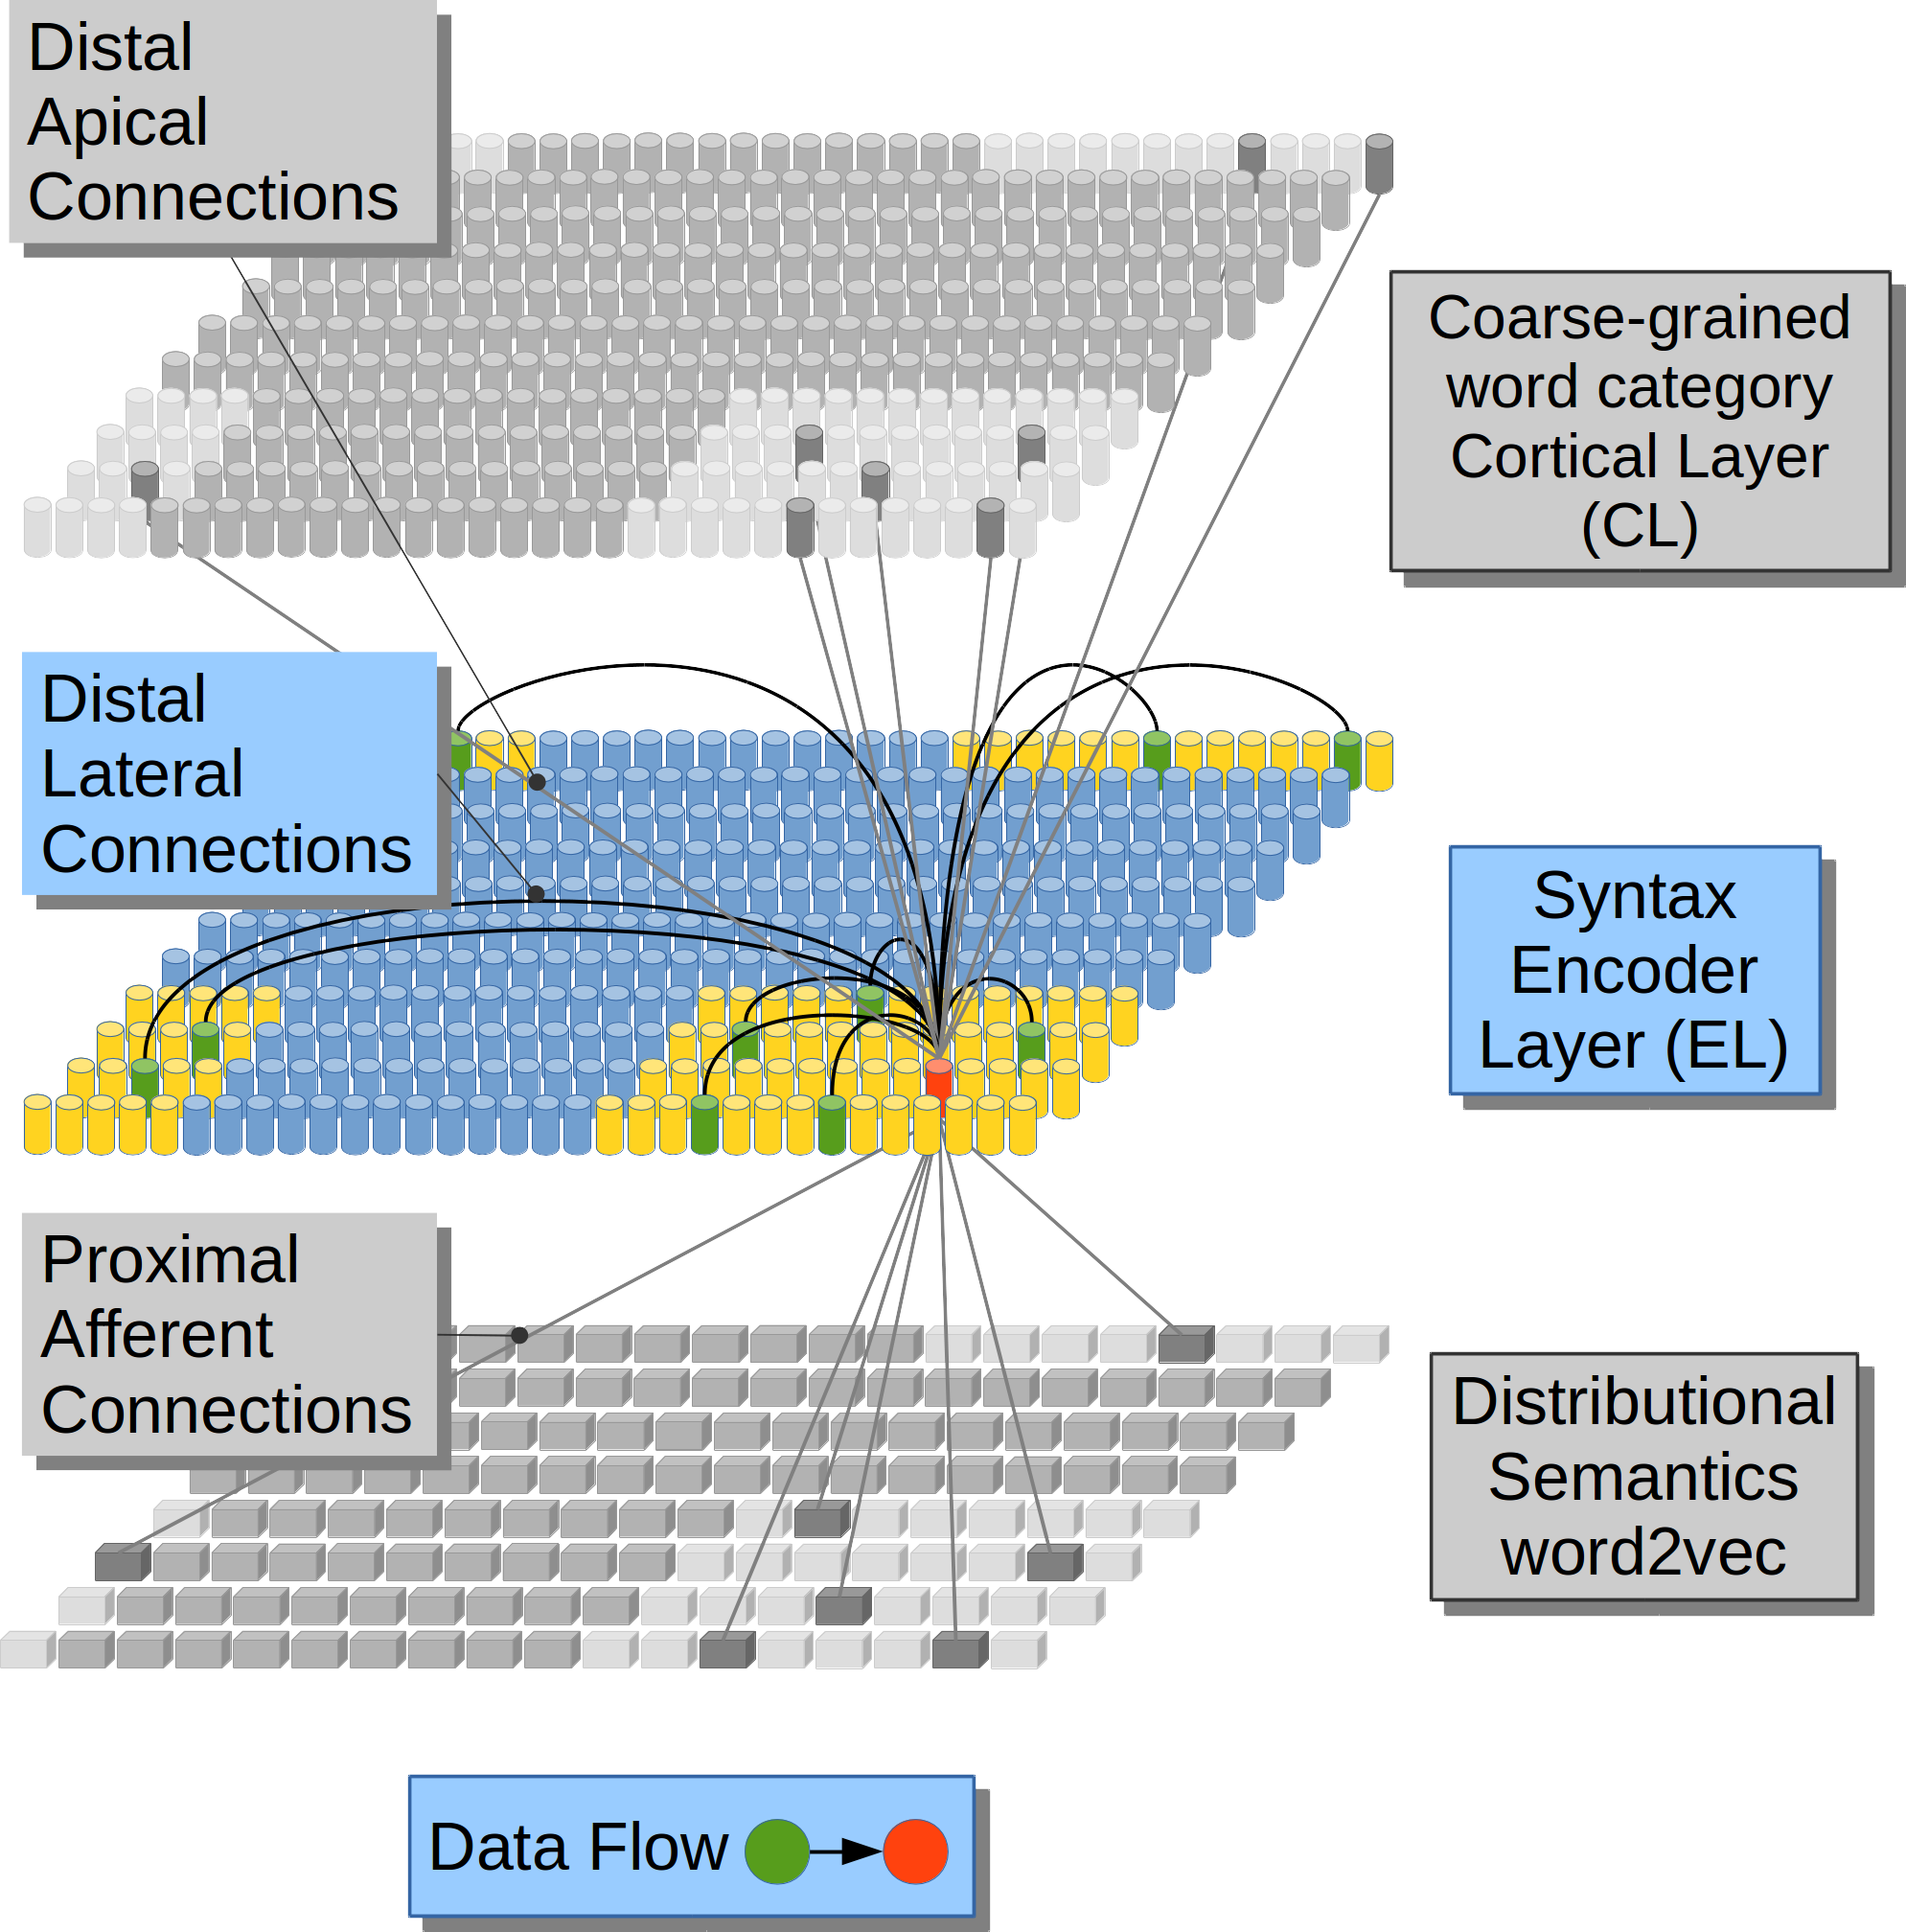
\includegraphics[width=0.6\textwidth]{EncoderConnections.png}
    \caption{Computational hypotheses.
    On the left we have the connection scheme for a \gls{cc} in the \gls{el}.
	    Each cylinder in the \gls{el} and in the \gls{cl} represents a \gls{cc} in neural tissue.
	    Each prism in Distributional Semantics (word2vec) represents a real-valued variable.
	    This is a visualization of a \gls{cc} (in red) and its three receptive fields (lateral in yellow and afferent and apical in light gray).
	Adapted from https://doi.org/10.1371/journal.pone.0217966 under CC-BY license, and
        brain image adapted from https://svgsilh.com/image/155655.html under CC0 1.0 license.}
    \label{fig:EncoderConnections}
\end{figure}

In our computational model \gls{ds} constraints from afferent dendrites excite clusters of neurons in the \glsfirst{el} stage in Fig.~\ref{fig:EncoderConnections}.
The \gls{el} may be related to a cortical patch composed by the \glsfirst{ba} 45 and the \gls{ba} 44 which are believed to contribute to syntactic processing \cite{Pallier2522, doi:10.1152/physrev.00006.2011, doi:10.1146/annurev-neuro-071013-013847}. The \gls{el} receives \glsfirst{ds} constraints in its afferent dendrites. This simulation feature accounts for information coming from \glspl{ba} 47 and 45 which are involved in semantic processing \cite{GOUCHA2015294, DECARLI2007933, PMID:15528098, NEWMAN201051}. \glspl{ds} information tends to activate clusters of units in the \gls{el}. Such activations are massive at first, covering all the plausible lexical hypotheses that the \glsfirst{ds} information conveys. All the lexical hypotheses activated by afferent dendrites are narrowed down by distal dendrites receiving previous activations from the very same \gls{el} (lateral) and by distal dendrites receiving coarse-grained word category information (apical)
which could be related to \gls{ba} 44 and part of \gls{ba} 6 which have a role in phonological processing \cite{Lee3942, PMID:27381836, HEIM2003285, PMID:18296070, AMUNTS200442}.
Distal connections partially depolarize specific neural units in the \gls{el} which will get a running start on their activations compared to neighboring units, when afferent information arrives. Partially depolarized units will activate faster than their counterparts, inhibiting their depolarization and, in this way, preventing them from firing. By means of such strategy, the \gls{el} generates \glspl{sdr} with a 99\% of sparsity, popping up only one choice among all the alternative unification links. We propose that in such way only one phrasal configuration remains active among the alternative binding candidates.

We assign coarse-grained syntax information to apical dendrites based on the primacy that some evidence confer to syntax
\cite{BORNKESSELSCHLESEWSKY200855,doi:10.1111/j.1749-818X.2008.00099.x,FRIEDERICI200278,doi:10.1152/physrev.00006.2011}, and on the fact that
apical dendrites receive feedback input \cite{Spruston2008PyramidalND} whose connectivity is usually related to modulatory functions--guiding effects produced by forward connections--\cite{news_hidden_2018, marques_functional_2018, Chen2009ForwardAB}.
Hence we assign \gls{ds} information a forward driving role in our model which is modulated by previously activated information from distal (apical and lateral) dendrites. Therefore we are accounting for the psycho-linguistic evidence supporting the primacy of syntax and we are also accounting for neurophysiological evidence providing a functional role to the apical tuft in pyramidal cells.

Thus, in the present work, we introduce a fully unsupervised approach in which constraints from different sources are correlated repeatedly until grammatically related word category generalization naturally emerges from the statistical properties of the stimulus. Our computational model does not apply any form of optimization guidance beyond Hebbian learning. It does not backpropagate errors, nor optimize weights based on hypothetical cost functions. 

An influential trend of compelling research is currently trying to explain how Back-Propagation might be carried out by neural tissue in the brain \cite{WHITTINGTON2019235}. Biologically questionable aspects of the Back-Propagation algorithm such as the lack of local error representation and the need of symmetry in forward and backward weights are addressed by sound neurocomputational theories \cite{10.7554/eLife.22901, Lillicrap_2016}. Although such theories contribute with powerful arguments favoring the fact that Back-Propagation could have been implemented by evolution in cortical tissue, empirical evidence is far from conclusive. We believe there is still a long way to go before we can assure that the complex requirements imposed by \emph{credit assignment}--the ultimate goal of Back-Propagation--could be a phenomenon occurring in cortical tissue. We are also skeptical regarding \gls{bptt} mechanisms in cortex given the demanding requirements they impose in its implementation. \gls{bptt} has particular problems specifically regarded to \gls{tca} which are not present in feedforward backpropagation \cite{LILLICRAP201982}.

In such regard, we remain cautious, keeping our model as simple as possible. We do not implement reinforcement mechanisms either. Instead, we feature strong evidence from current deep neural network approaches in which spontaneous emergence of abstract concepts seems to be a new landmark for \gls{ml}. For instance, it has been seen that biologically-inspired deep neural networks spontaneously gain number sense even when trained only to recognize objects in an image \cite{Nasreaav7903}. Moreover, using the same computational hypotheses than in the present work, our group has shown how phonetic invariance and generalization spontaneously emerges from the sequential constraints imposed by the statistical structure of the stimulus. Avoiding the utilization of optimization guidance mechanisms--such as supervision or reinforcement--we could significantly improve the \gls{svm} phonetic classification performance of stimuli seriously impaired by different levels of white noise, reverberation and changes in pitch and voices \cite{10.1371/journal.pone.0217966}.

In the present work, we advance an improved version of the neurocomputational model previously developed in \cite{10.1371/journal.pone.0217966}.
In its present form, afferent dendrites drive \glsfirst{ds} Text Embedding information, while lateral dendrites receive sequential syntactic restrictions but, more importantly, we incorporate apical dendrites which simulate backward connectivity from distant cortical patches carrying coarse-grained word category information which has been shown to be phonologically informed \cite{doi:10.1207/s15327078in1002_5, lohmann_phonological_2017}. Backward connectivity has been seen to be prevalent in brain cortex, usually related to modulatory functions, driving effects produced by forward connections, and transcending more than one cortical level \cite{news_hidden_2018, marques_functional_2018, Chen2009ForwardAB}. Therefore, we show how our model--specifically the \gls{el}--in its current form, displays the acquisition of complex cognitive phenomena such as grammatically relevant categories, improving the \gls{svm} classification of grammatical functions within a sentence, compared to current word embedding representations \cite{Mikolov:2013:DRW:2999792.2999959, mikolov2013linguistic, journals/corr/abs-1301-3781}.

In this paper we research some features of the \gls{lifg} information processing gradient in order
to settle the stream of linguistic information in our model.
Replicating the neurophysiology present in the \gls{lifg} complex is beyond the scope of this research.
We impose biological constraints to such information processing stream by means of general--and widely acknowledged--biological claims basing our reasoning on the homogeneity found throughout cortical tissue in the brain \cite{Carlo1488}.
}
















\iftoggle{DEBUG}{
\section{Materiales y métodos}
}{
\section{Materials and methods}
}

















\iftoggle{DEBUG}{
\subsection{Modelo Computacional}

Proponemos un enfoque computacional inspirado en la biología de la corteza de los mamíferos el que simula un parche de tejido cortical e incorpora organización columnar, formación microcolumnar espontánea, activaciones como \glsfirst{sdr} las que se ha demostrado que derivan de las depolarizaciones dendríticas parciales \gls{nmda} \cite{Antic2010TheDO,Major2013ActivePO,10.3389/fncir.2016.00023}, y la adaptación a activaciones contextuales.
Simulamos células piramidales con conexiones próximas desde ramas dendríticas aferentes y conexiones distales desde ramas dendríticas apicales y laterales \cite{10.1371/journal.pone.0217966}.

En nuestro modelo computacional consideramos células piramidales en las capas II/III y la segregación de sus ramas dendríticas dentro de diferentes dominios.
Dichos dominios en la célula reciben diferentes entradas sinápticas y tienen sinapsis con excitabilidad, modulación y propiedades de plasticidad específicas \cite{Spruston2008PyramidalND}.
Las dendritas basales y apicales próximas de las células en las capas II/III toman entradas desde células en la capa IV y también reciben excitación desde circuitos locales las cuales procesan entradas excitatorias desde fuentes locales.
La cresta apical--por otro lado--colecta entradas desde otras regiones corticales y también recibe entradas talámicas no específicas que controlan la sensibilidad o respuesta de la célula a entradas más próximas \cite{10.1093/cercor/bhh065}.

En relación a la conectividad aferente próxima en la \gls{el}, la evidencia muestra que las capas II/III predominantemente acepta entradas excitatorias inter-laminares--principalmente orientadas verticalmente--desde células en la capa IV.
Por otro lado, el uso de la conectividad distal lateral toma en cuenta las neuronas de las capas II/III que también reciben entradas desde otras neuronas en las capas II/III a través de conexiones laterales extensas \cite{BANNISTER200595}.
Finalmente y a manera de puerta de salida, muchas neuronas de las capas II/III proyectan hacia niveles más altos de la corteza \cite{THOMSON1998669}.

Así, la información desde ramas dendríticas distales en nuestro modelo--las que son laterales y apicales--de antemano produce una depolarización parcial en algunas unidades celulares en una \gls{cc} (Fig. \ref{fig:EncoderConnections}).
Por otro lado, la información desde ramas dendríticas próximas--las cuales son aferentes--produce una depolarización completa de un cúmulo de unidades celulares en una \gls{cc}, pero si existe una cantidad suficiente de neuronas excitadas aferentemente que ya han sido parcialmente depolarizadas por dendritas apicales y/o laterales, tales unidades dispararán antes inhibiendo otras unidades en los cúmulos y evitando por tanto su disparo.
Con este mecanismo sólo un número reducido de unidades se activan produciendo así patrones dispersos de activación en nuestro modelo.
Esta teoría computacional ha sido introducida en \cite{10.3389/fncir.2016.00023}, mostrando la capacidad de aprendizaje de secuencias no supervisado y en línea \cite{Cui:2016:COS:3030654.3030660}.

El procesamiento de información en las capas II/III concierne a la \emph{inferencia secuencial} la cual requiere la interacción de sus conexiones laterales y apicales con la entrada ascendente (\emph{bottom-up}).
La evidencia sugiere que las neuronas en las capas II/III podrían llevar a cabo computaciones similares a las desarrolladas en nuestro modelo. Se ha reportado que las conexiones horizontales de larga distancia hacia células piramidales en las capas II/III exhiben propiedades diferentes a las de las conexiones verticales \cite{Yoshimura1931}.
También se ha sugerido que las proyecciones de las neuronas de la capa IV hacia las neuronas piramidales en las capas II/III actúan como una compuerta para la difusión lateral de la excitación en las capas II/III \cite{doi:10.1113/jphysiol.2001.012959}.
Basándonos en tales evidencias asignamos a la \gls{ds} un rol conductor que es modulado por activaciones sintácticas previas desde dendritas apicales y por restricciones laterales previas generadas en la misma \gls{el}.

Algunas características importantes para resaltar en nuestro enfoque computacional \cite{10.1371/journal.pone.0217966} son: (i) las dendritas aferentes próximas no determinan una unidad neuronal a disparar pero determinan su probabilidad de hacerlo, (ii) las ramas dendríticas distales son elementos computacionales independientes que contribuyen al disparo somático por medio de impulsos dendríticos y (iii) las fallas de predicción en la red producen un fenómeno llamado \gls{mfe} que se manifiesta con la activación de muchas neuronas en una \gls{cc} perjudicando la formación de \gls{sdr_pl}.

En referencia a la naturaleza aleatoria en nuestro enfoque computacional, estudios previos ya han incorporado características estocásticas a modelos biológicamente plausibles de dinámica neuronal \cite{harrison_l.m_stochastic_2005}.
Adicionalmente, la autonomía de las dendritas neuronales como elementos de computación independientes ya ha sido establecida mostrando que las dendritas neuronales exhiben una gama de mecanismos lineales y no lineales que les permiten implementar computaciones elementales \cite{poirazi_dendritic_2015, PAYEUR201978}.
La compartimentación de unidades neuronales individuales (capas II/III) en nuestro modelo no se limita solamente a configuraciones dendríticas completas; por el contrario nos motivan estudios científicos recientes afirmando que compartimentos dendríticos individuales pueden realizar una computación específica--como la operación OR exclusiva--que había sido considerada de imposible realización por sistemas de una única neurona \cite{Gidon83}.
Finalmente los \gls{mfe_pl} en el modelo explican un fenómeno de integración en el cual una combinación de restricciones diferentes convergen incoherentemente y producen la activación masiva de un cúmulo neuronal en una \gls{cc} de la \gls{el}.
Cuando la \gls{el} no puede integrar la información proveniente de distintas restricciones lingüísticas de manera fluida, este activa más hipótesis--es decir, más configuraciones frasales--para poder fusionar la información dentro del contexto oracional secuencial subsecuente más fácilmente. 

Fenómenos de activación como los \gls{mfe_pl} impiden la formación de \gls{sdr_pl}. Sin embargo cuando la \gls{el} predice correctamente el flujo secuencial de la información que viene desde diferentes restricciones lingüísticas, producirá \gls{sdr_pl} continuamente y la activación secuencial correrá de manera fluida.
Las \gls{sdr_pl} exhiben propiedades matemáticas interesantes, las que les dan un gran rechazo al ruido y una alta tolerancia a las fallas \cite{DBLP:journals/corr/AhmadH15}.
Se ha mostrado que el cerebro utiliza patrones de activación dispersa para procesar información en todos los mamíferos, desde ratas hasta humanos \cite{barth_experimental_2012}.
}{
\subsection{Computational Model}

We propose a computational approach inspired in the biology of the mammalian neocortex which simulates a patch of cortical tissue and incorporates columnar organization, spontaneous micro-columnar formation, \glsfirst{sdr} activations which have shown to be derived from partial \gls{nmda} dendritic depolarization \cite{Antic2010TheDO,Major2013ActivePO,10.3389/fncir.2016.00023}, and adaptation to contextual activations. We simulate pyramidal cells with proximal connections from afferent dendritic branches and distal connections from lateral and apical dendritic branches \cite{10.1371/journal.pone.0217966}.

In our model we account for layer II/III pyramidal cells processing and the segregation of their dendritic trees into different confined domains.
Different dendritic domains in the cell receive distinct synaptic inputs and have synapses with specific excitability, modulation and plasticity properties \cite{Spruston2008PyramidalND}.
The basal and proximal apical dendrites of cells in layer II/III take inputs from layer IV cells and also receive local-circuit excitation
which process excitatory inputs from local sources.
The apical tuft--on the other hand--collects inputs from other cortical areas and also receives nonspecific thalamic inputs
which control responsiveness to more proximal inputs \cite{10.1093/cercor/bhh065}.

Regarding proximal afferent connectivity in the \gls{el}, evidence shows that layer II/III predominately accepts inter-laminar--mostly vertically oriented--excitatory inputs from the stellate cells in layer IV. On the other hand the use of lateral distal connectivity accounts for layer II/III neurons which also receive excitatory inputs from other layer II/III neurons through extensive lateral connections \cite{BANNISTER200595}. Finally, and as an output gateway, many layer II/III neurons project to higher levels of cortex \cite{THOMSON1998669}.

Hence the information from distal dendritic branches in our model--which is lateral and apical--produces, in advance, a partial depolarization in some cell units in a \gls{cc}  (Fig. \ref{fig:EncoderConnections}). On the other hand, information from proximal dendritic branches--which is afferent-- produces a complete depolarization of a cluster of cell units in a \gls{cc}, but in the event that enough afferently excited units have already been partially depolarized by lateral and/or apical dendrites, such units would fire before inhibiting other units in the cluster and preventing them from firing. With this mechanism, only a reduced number of units become active, producing a sparse pattern of activation in our model. This neurocomputational theory has been introduced in \cite{10.3389/fncir.2016.00023}, showing continuous online and unsupervised sequence learning capabilities \cite{Cui:2016:COS:3030654.3030660}.

Information processing in layer II/III concerns \emph{sequential state inference} which requires the interaction of their lateral and apical connections with the bottom-up input. Evidence suggest that neurons in layer II/III could endeavour similar computations to the one developed by our model. \cite{Yoshimura1931} reported that long distance horizontal connections to pyramidal cells in layer II/III exhibit different properties than those from vertical connections.
\cite{doi:10.1113/jphysiol.2001.012959} also suggested that the projections of layer IV spiny neurons to layer II/III pyramidal neurons act as a gate for the lateral spread of excitation in layer II/III. Based on such evidence we assign \gls{ds} a driving role which is modulated by previous syntax activations from apical dendrites and previous lateral constraints generated in the same \gls{el}.

Some important remarks in reference to our computational approach \cite{10.1371/journal.pone.0217966} are: (i) proximal afferent dendrites do not determine a neuron to fire, instead, they bias its probability of doing so, (ii) distal dendritic branches are independent computing elements that contribute to somatic firing by means of dendritic spikes, and (iii) prediction failures in the network produce a phenomenon called \gls{mfe} which manifests with the activation of many neurons in a \gls{cc} impairing \glspl{sdr} formation.

In reference to the random nature imprinted in the computational approach, previous studies have already incorporated stochastic forces to biologically plausible models of neuronal dynamics \cite{harrison_l.m_stochastic_2005}. In addition, the autonomy of neural dendrites as independent elements of computation has already been posed, showing that neuronal dendrites exhibit a range of linear and nonlinear mechanisms that allow them to implement elementary computations \cite{poirazi_dendritic_2015, PAYEUR201978}. The compartmentalization of individual (layer II/III) neural units in our model is not limited to only complete dendritic configurations; we are rather motivated by recent scientific studies claiming that individual dendritic compartments can perform a specific computation--exclusive OR--that mathematicians had previously regarded as an unsolvable problem by single-neuron systems \cite{Gidon83}.
Finally \glspl{mfe} in the model explain integration phenomena in which a combination of different constraints converges incoherently and produces the massive activation of a neuron cluster in the \glspl{cc} of the \gls{el}. When the \gls{el} cannot fluently integrate information coming from different linguistic constraints, it activates more hypotheses--i.e more phrasal configurations--as to be able to easily fuse subsequent information coming within the sequential sentence context.

An activation phenomenon such as the \glsfirst{mfe} impedes \glspl{sdr} formation. However, when the \gls{el} correctly predicts the sequential stream of information coming from different constraints, it continuously produces \glspl{sdr} and the sequential activation runs smoothly. \glspl{sdr} exhibit interesting mathematical properties which give them high noise rejection and fault tolerance \cite{DBLP:journals/corr/AhmadH15}. It has been shown that the brain uses sparse patterns of activation to process information in all mammals, from mice to humans \cite{barth_experimental_2012}.
}






\iftoggle{DEBUG}{
\subsection{Restricciones Aferentes de Semántica Distribucional}

Generamos restricciones de \gls{ds} utilizando un enfoque de \emph{Word Embeddings}. \emph{Word Embeddings} es un conjunto de técnicas de \gls{nlp} en las que palabras o frases se mapean a vectores de números reales.
En este trabajo utilizamos específicamente word2vec el cual toma un gran corpus de texto como entrada y produce un espacio de vectores que usualmente tiene cientos de componentes.
Se asigna cada palabra en el corpus a un vector correspondiente en el espacio. La hipótesis principal es que palabras que aparecen de forma recurrente en posiciones próximas en el texto se ubicarán de manera próxima en el espacio semántico (espacio de vectores de \gls{ds}).
Esta hipótesis se basa en la \glsfirst{ds} en lingüística la que se deriva de la teoría semántica del uso del lenguaje \cite{doi:10.1080/00437956.1954.11659520}.
La salida de tal modelo es un espacio semántico multidimensional con propiedades semánticas poderosas \cite{mikolov2013linguistic, journals/corr/abs-1301-3781, Mikolov:2013:DRW:2999792.2999959}.
En este trabajo utilizamos vectores pre-entrenados obtenidos desde parte del dataset \emph{Google News} (alrededor de 100 billones de palabras).
El modelo contiene vectores de 300 dimensiones para 3 millones de palabras y frases \cite{noauthor_google_nodate}.

La mayor proyección excitatoria recibida por las neuronas de las capas II/III está en su mayoría compuesta por axones verticalmente orientados y en mayor parte intra-columnares desde las neuronas en la capa IV \cite{10.3389/neuro.01.1.1.002.2007,Lbke2007ExcitatorySF}.
Generalmente se acepta a la capa IV como una entrada directa a las regiones corticales \cite{doi:10.1177/1073858407305201}.
Consecuentemente interpretamos tal característica microcircuital como una compuerta de entrada desde la cual las neuronas en las capas II/III reciben excitación aferente próxima desde la \gls{ds}.

Siguiendo la evidencia arriba expuesta implementamos las dendritas aferentes por medio de un \gls{som} \cite{Kohonen:1988:SFT:65669.104428, Kohonen1989SelforganizationAA}.
Cada \gls{cc} en la \gls{el} simula una dendrita aferente próxima utilizando un \gls{som} como muestran las Figs. \ref{fig:EncoderProximalConnections1} A y \ref{fig:EncoderProximalConnections1} B. Cada \gls{cc} recibe una muestra reducida de componentes word2vec.

\begin{figure}[ht!]
    \centering
    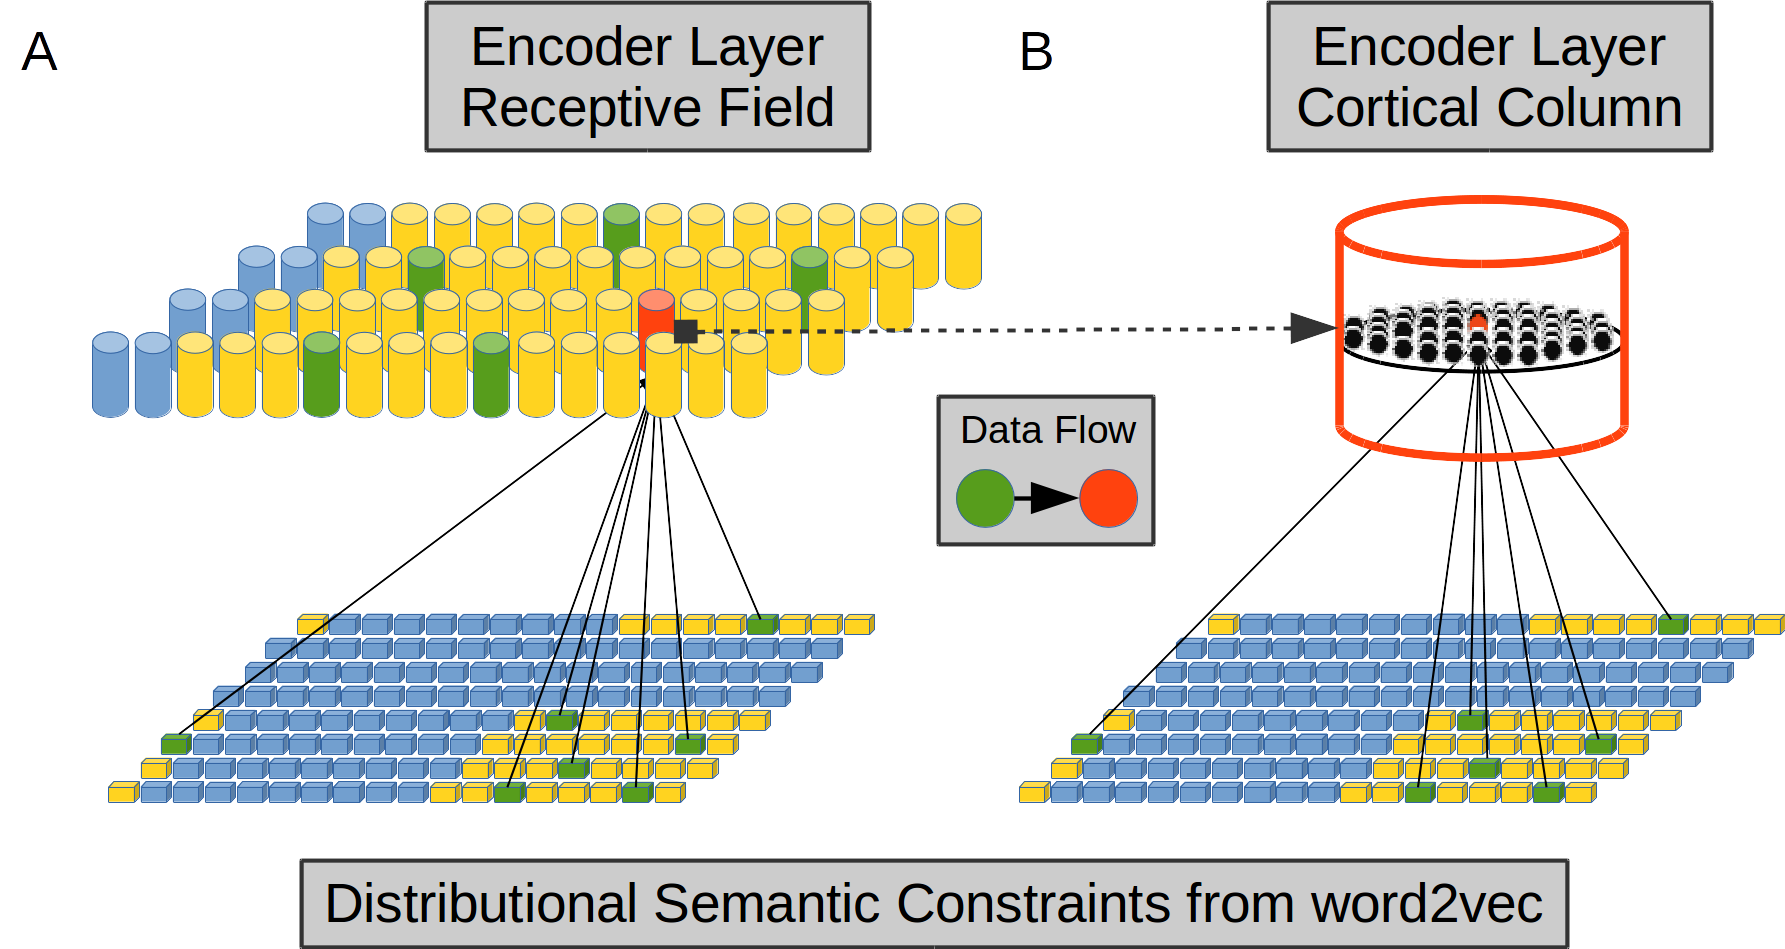
\includegraphics[width=0.8\textwidth]{EncoderProximalConnections1.png}
    \caption{Conexiones aferentes próximas en la \glsfirst{el}. Cada \gls{cc} en la \gls{el}--ejemplificada en rojo aquí--tiene su campo receptivo sobre el espacio semántico word2vec--en amarillo.
    \textbf{(A)} Un conjunto de componentes de word2vec--en verde dentro del campo receptivo--se selecciona aleatoriamente para conectarse con una \gls{cc}.
    \textbf{(B)} Cada unidad neuronal en una \gls{cc} se conecta con el mismo conjunto de componentes de word2vec. Basamos esta configuración de conectividad en la orientación vertical y en la configuración prominentemente intra-columnar de los axones aferentes recibidos desde la capa IV.
    Imagen adaptada de \url{https://doi.org/10.1371/journal.pone.0217966 bajo licencia CC-BY}.}
    \label{fig:EncoderProximalConnections1}
\end{figure}

El uso de un \gls{som} por \gls{cc} en nuestro modelo simula la interacción lateral intra-columnar próxima, la \gls{ltp}, la \gls{ltd} y la organización vertical de bandas celulares con propiedades de respuesta similares \cite{mountcastle_1955,Haueis2016}.
En cada \gls{cc} en nuestro modelo, cúmulos de unidades neuronales que responden a restricciones semánticas similares emergen de manera espontánea desde el proceso de aprendizaje.
Esto tiene correlato con la organización \emph{tonotópica}, \emph{retinotópica} o \emph{somatotópica} en la corteza cerebral.
Con tal mecanismo también estamos teniendo en cuenta \emph{el conjunto completo de columnas con orientación y el dominio ocular izquierdo y derecho} \cite{doi:10.1002/cne.901580305} el cual simulamos funcionalmente desde el punto de vista del procesamiento de la información semántica.
En nuestro enfoque de modelado tomamos el concepto de columna cortical como una \emph{unidad elemental de organización} de toda la corteza cerebral \cite{doi:10.1152/jn.1957.20.4.408,Mountcastle1978AnOP,10.1093/brain/120.4.701}. 


Las Figs. \ref{fig:CorticalColumnSOM} y \ref{fig:CorticalColumnTrainedSOM} muestran como se relaciona el espacio de la \gls{ds} en word2vec y cada \gls{cc} en la \gls{el}.
En la Fig. \ref{fig:CorticalColumnSOM} la dendrita aferente de la \gls{cc} está en su estado inicial y su sub-espacio semantico correspondiente, muestreado desde word2vec, es representado por varias palabras deperdigadas de fondo.
 
\begin{figure}[ht!]
    \centering
    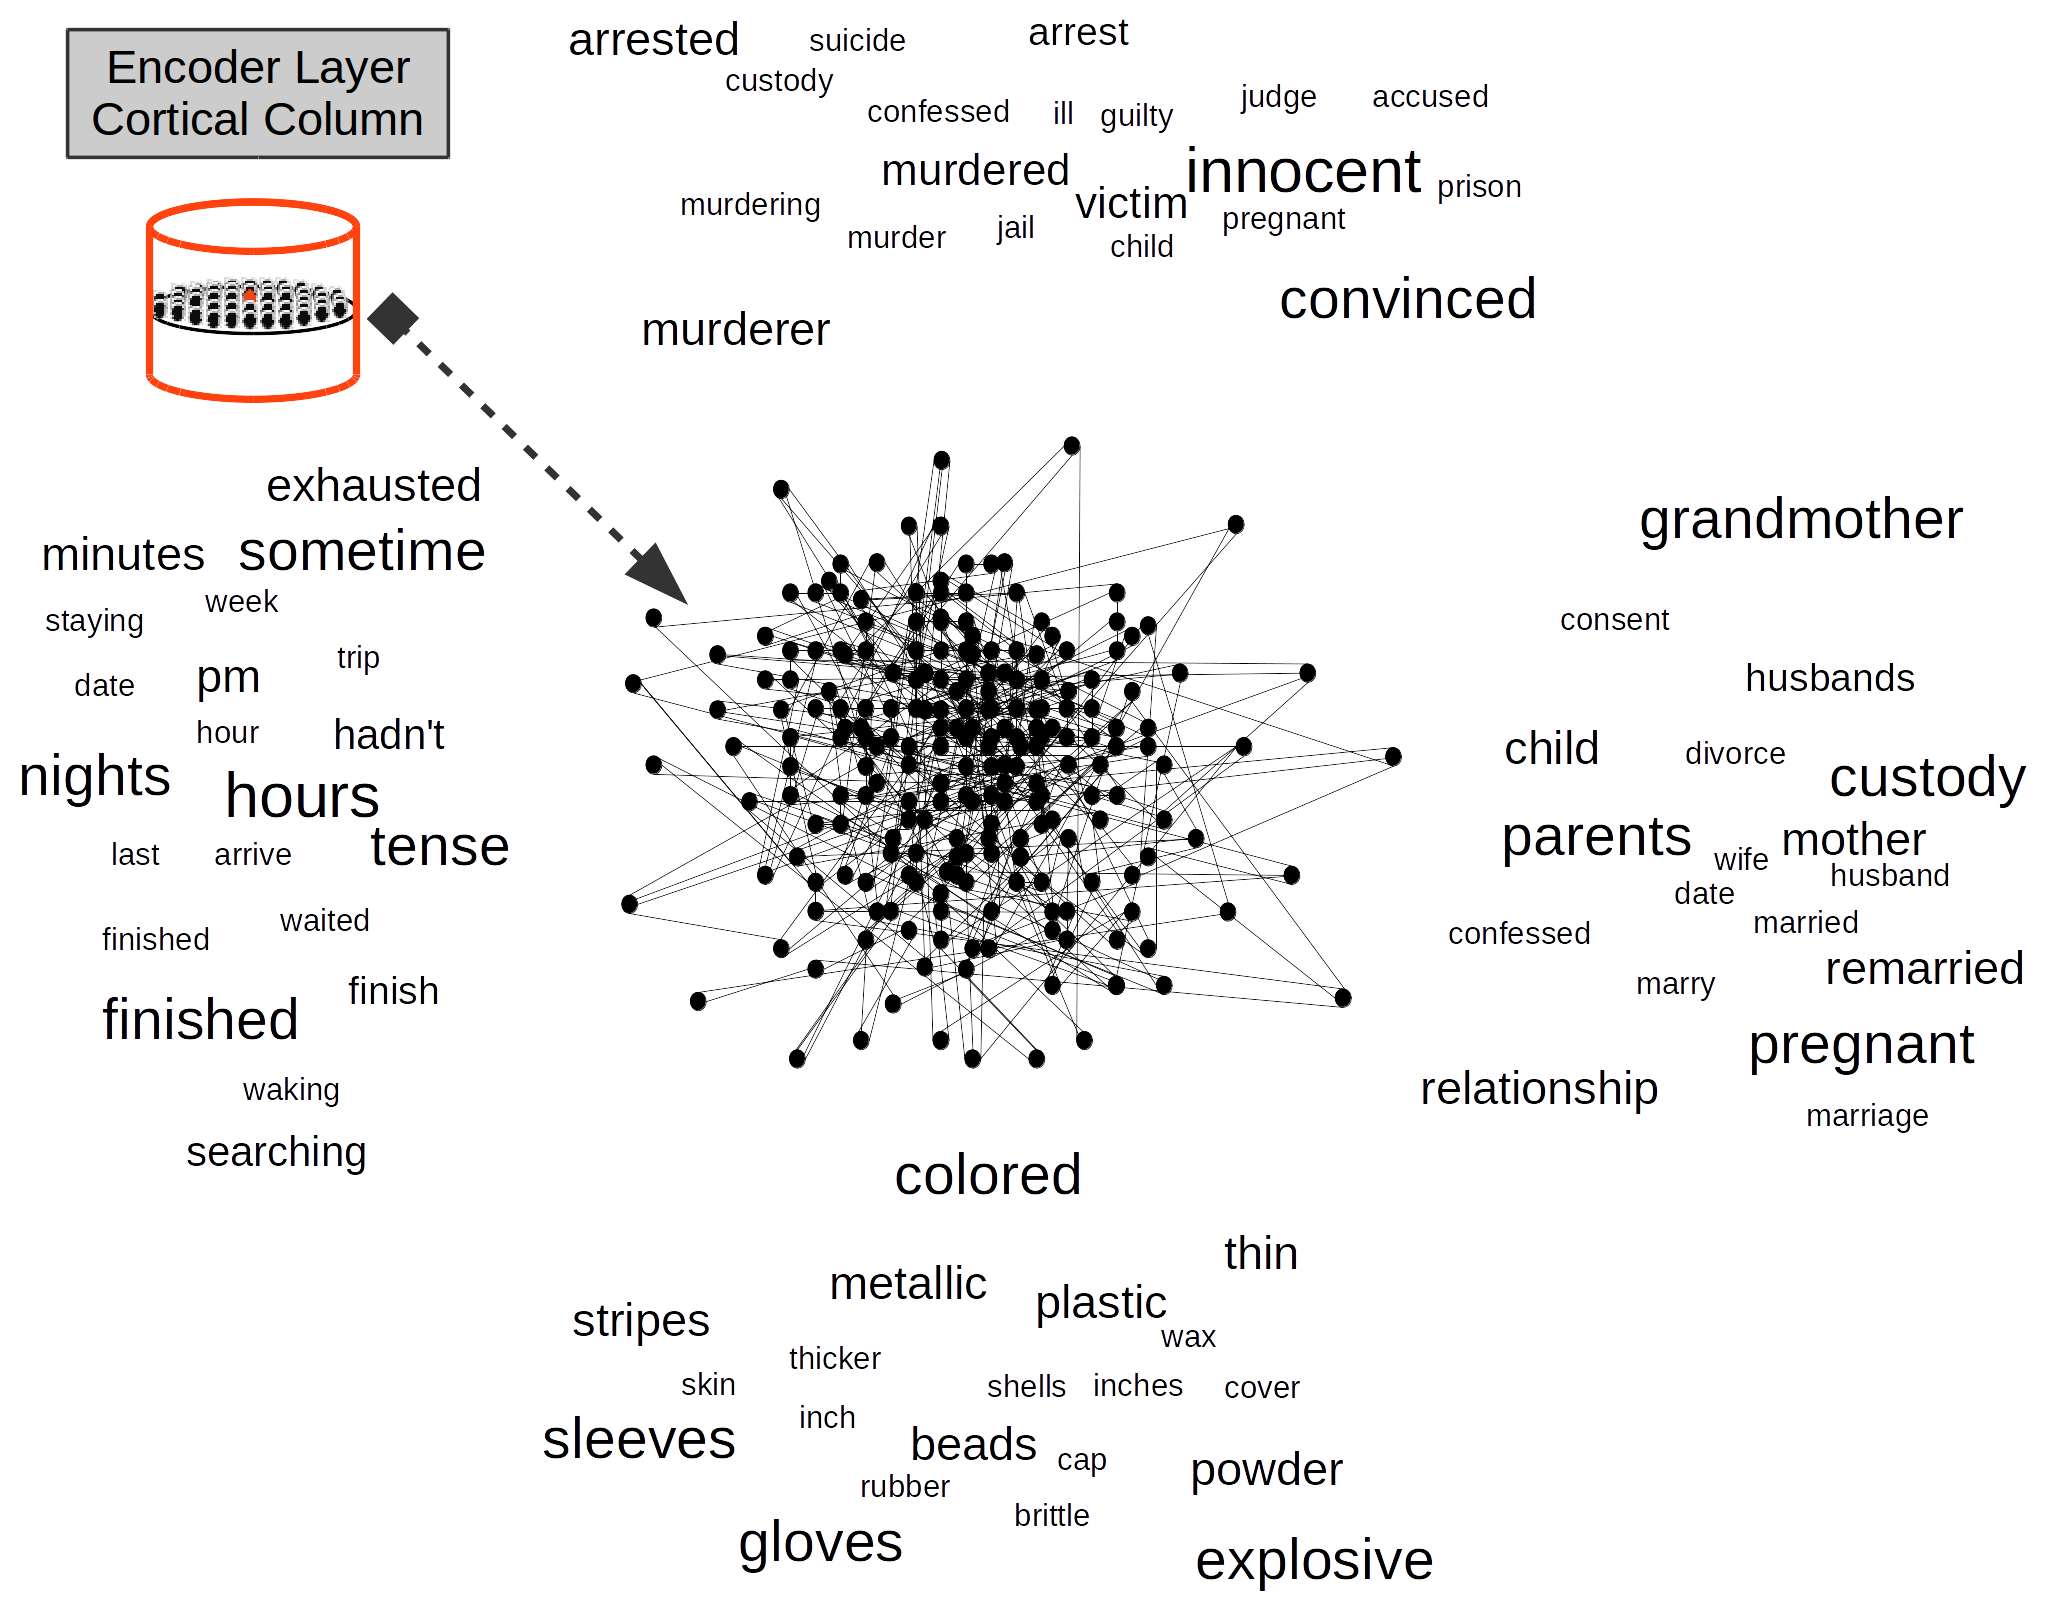
\includegraphics[width=0.8\textwidth]{CorticalColumnSOM.png}
    \caption{La \glsfirst{cc} en la \glsfirst{el} y su dendrita aferente próxima cuyas sinapsis se simulan  por medio de un \glsfirst{som}. Cada \gls{cc} en la \gls{el}--ejemplificada aquí en color rojo--tiene su campo receptivo sobre word2vec como un sub-espacio semántico representado por palabras desperdigadas en el fondo. Los pesos sinapticos del \gls{som} están en su estado inicial. Imagen adaptada de \url{https://doi.org/10.1371/journal.pone.0217966 bajo licencia CC-BY}.}
    \label{fig:CorticalColumnSOM}
\end{figure}

Cada conjunto de conexiones aferentes en una \gls{cc} determina un enrejado bidimensional de 15 por 15 unidades neuronales.
El sub-espacio semántico muestreado tiene 31 componentes de valor real.
En la Fig. \ref{fig:CorticalColumnTrainedSOM}--una vez que la dendrita aferente de la \gls{cc} ha sido entrenada--el enrejado neuronal distribuye sus unidades neuronales en todo el sub-espacio semántico. En tal caso, cada palabra en el sub-espacio semántico tendrá su representaciín en recursos neuronales y las palabras con con proximidad semántica en el sub-espacio semántico serán representadas por recursos neuronales con proximidad física en el enrejado. La preservación de la vecindad en los mapas auto-organizados constituye una propiedad importante que resulta de utilidad para preservar las relaciones semánticas del sub-espacio original en el nuevo espacio en el enrejado de una \gls{cc} en la corteza \cite{557663}. Sin embargo, más importante es que el remapeo de la \gls{ds} desde el sub-espacio de word2vec a la dimensionalidad reducida del enrejado neuronal revela relaciones ocultas entre terminos en el sub-espacio original como es el caso que se da en \gls{lsa} \cite{key:article}.

\begin{figure}[ht!]
    \centering
    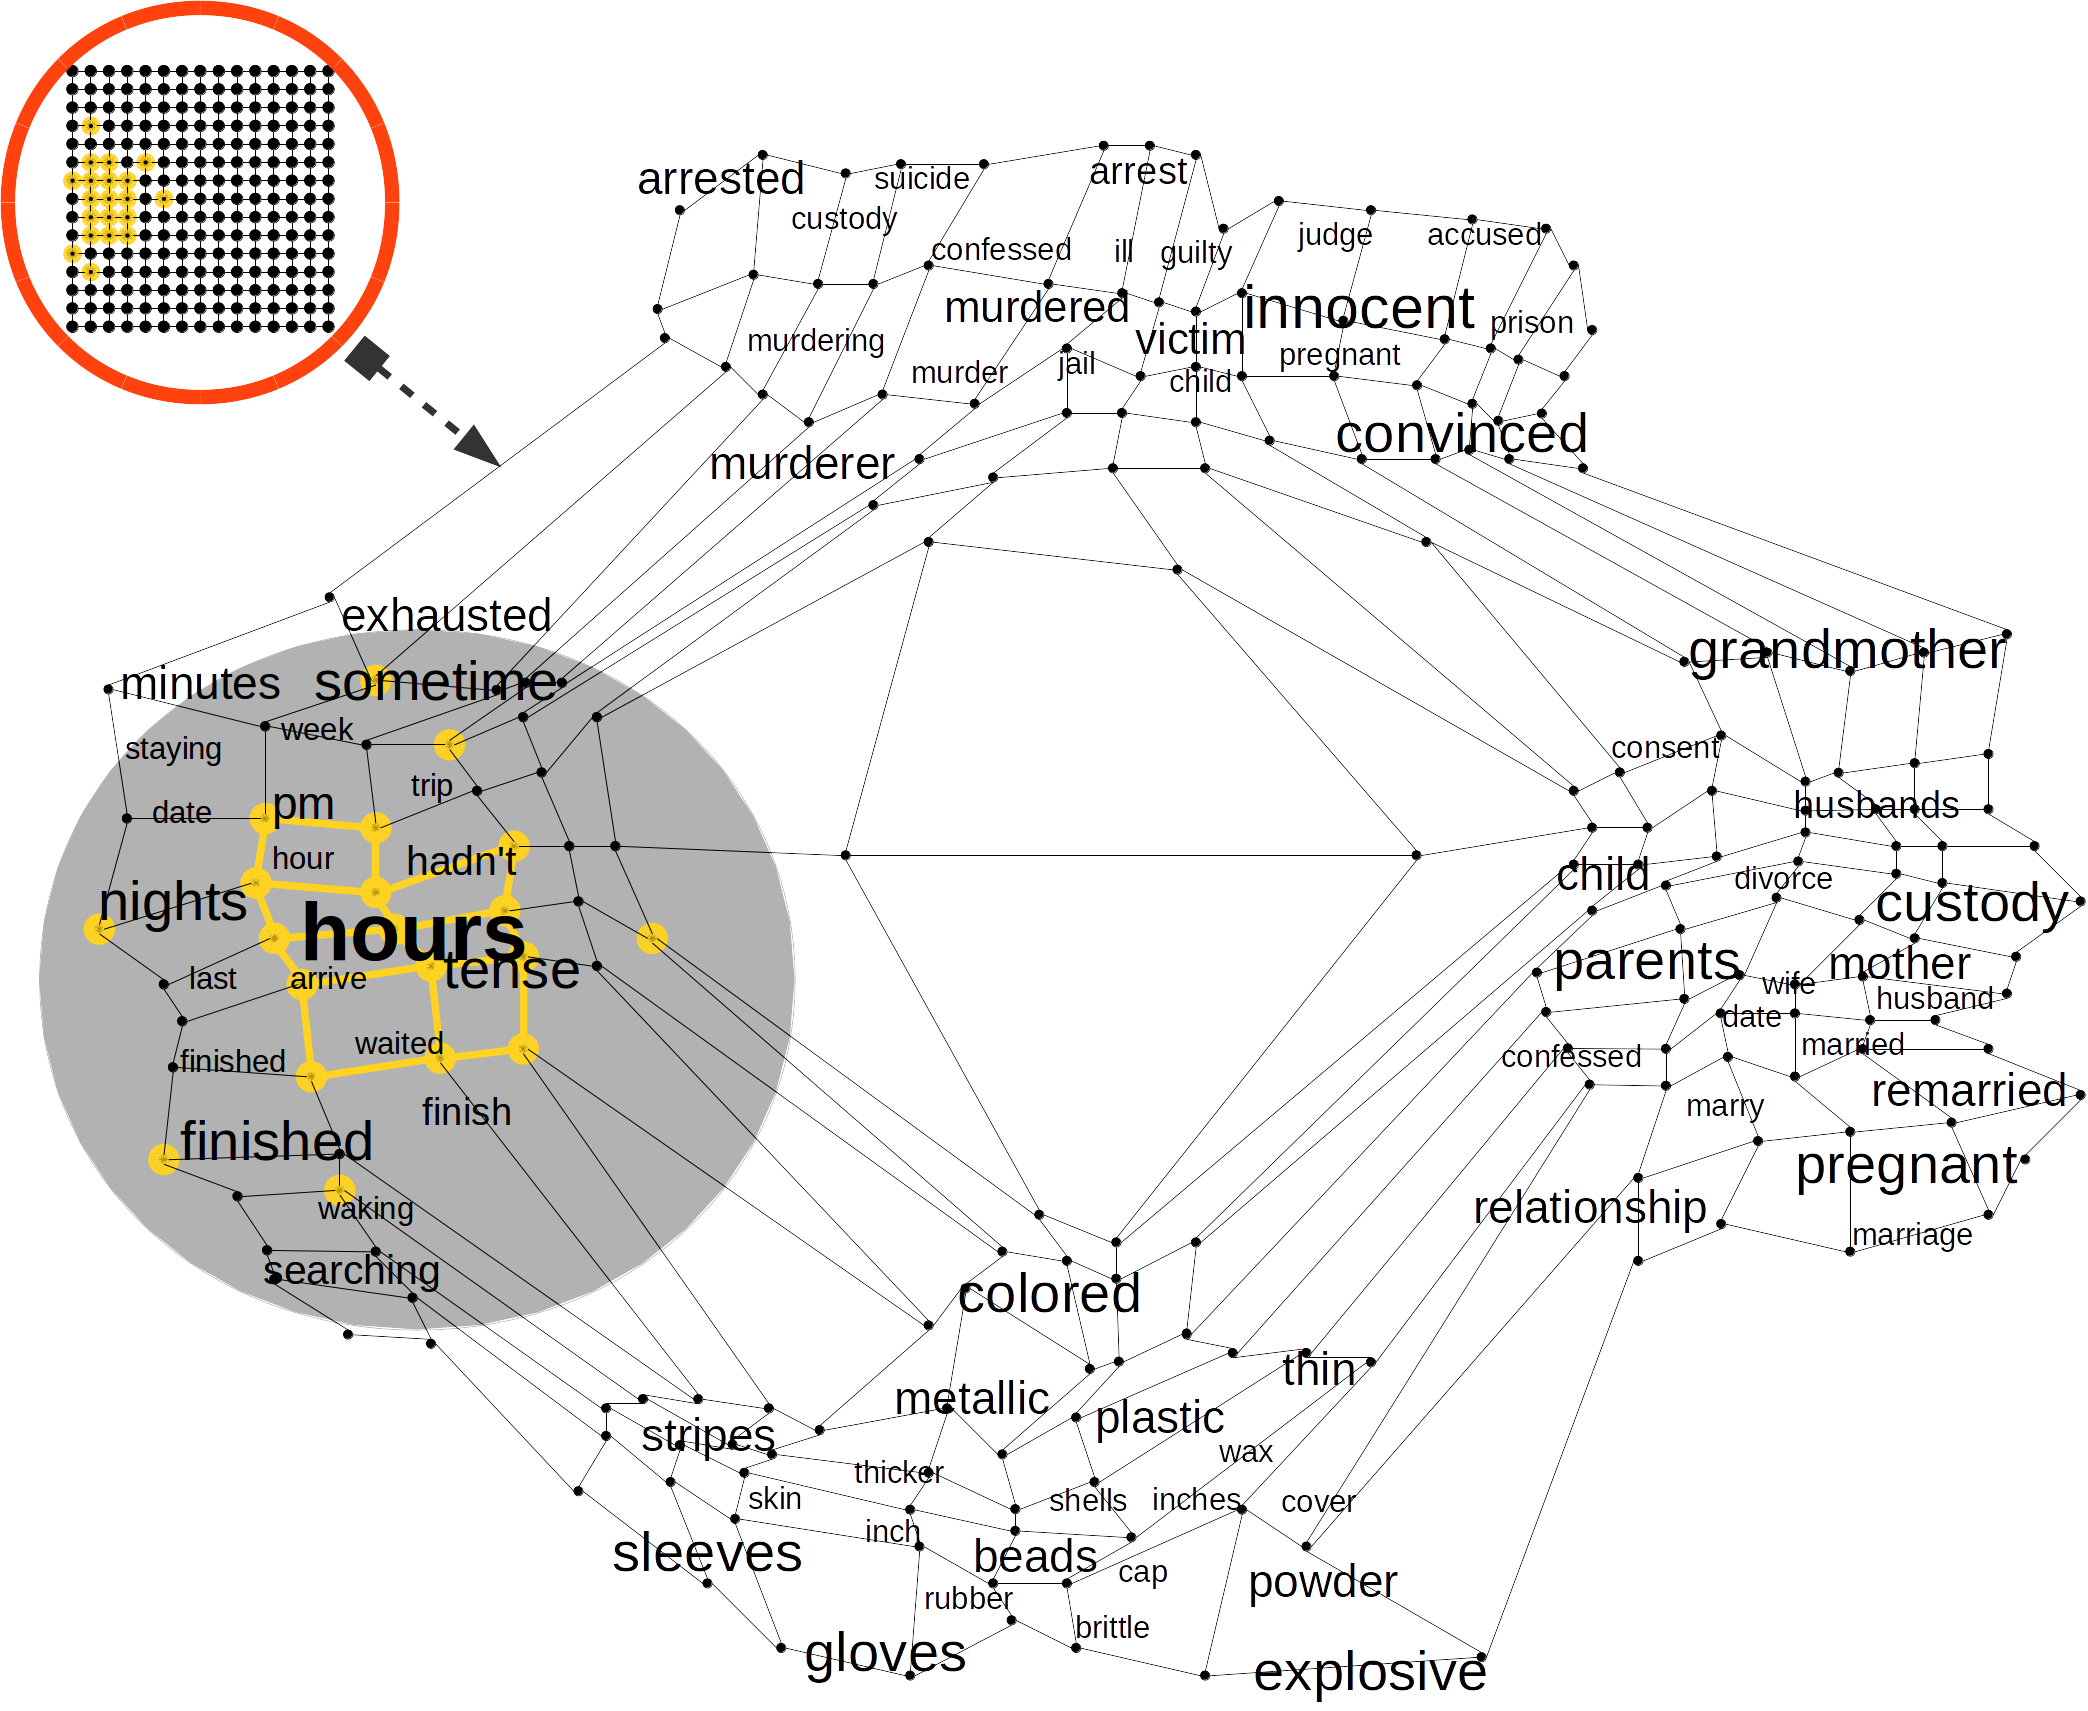
\includegraphics[width=0.8\textwidth]{CorticalColumnTrainedSOM.png}
    \caption{Un \glsfirst{som} entrenado en las conexiones aferentes próximas de una \glsfirst{cc}. El \gls{som} es un enrejado bidimensional de 225 unidades neuronales (15 por 15 unidades neuronales). El \gls{som} se adapta para representar el sub-espacio de la \glsfirst{ds} de word2vec. Una vez entrenado, un \gls{som} en una \gls{cc} distribuye sus unidades neuronales por todo el sub-espacio de \gls{ds} muestreado desde word2vec. El algoritmo del \gls{som} conserva la topología semántica del sub-espacio de \gls{ds} imprimiéndola en el enrejado de unidades neuronales. Cada palabra en el sub-espacio de \gls{ds} tiene su representación neuronal y palabras con más similitud semántica  se representan por unidades neuronales con gran proximidad física en el enrejado.}
    \label{fig:CorticalColumnTrainedSOM}
\end{figure}

Una vez que las dendritas aferentes han aprendido la distribución estadística inmersa en los diferentes su-espacios de \glsfirst{ds}, cada \gls{cc} en la \gls{el} tiene su representación privada de su sub-espacio de \gls{ds} desde word2vec.
El advenimiento de la representación de la \gls{ds} desde cierta palabra en word2vec establece un patrón de activación en un cúmulo de unidades neuronales dentro de cada \gls{cc} (Fig. \ref{fig:CorticalColumnTrainedSOM}).
De esta forma, cada restricción de \gls{ds} desde word2vec será representada de manera distribuida en la \gls{el}.
La representación semántica de cada palabra activará un cúmulo de unidades neuronales en cada \gls{cc}, y el contenido en \gls{ds} de tal palabra será distribuido en el parche cortical simulado por la \gls{el}.
Evidencia significativa muestra que el contenido semántico de las palabras se distribuye a lo largo del tejido cortical \cite{huth_natural_2016}.
Por ejemplo, una palabra como \emph{top} no sólo puede activar una región relacionada con la vestimenta y la apariencia, sino que también activa una región relacionada a los números y medidas y quizás también una región relacionada a las construcciones y lugares.
Por otro lado, también se ha mostrado que palabras con contenido semántico similar son mapeadas en regiones próximas de la corteza \cite{pub.1005704802}.
Por ejemplo, en la unión temporoparietal derecha un parche cortical pequeño responde a palabras como \emph{esposa, madre, embarazada, familia, amigos, hermano} etc, mientras que un parche muy cercano responde a palabras como \emph{familia} y \emph{esposa} pero también responde a palabras--relacionadas en cierta forma semánticamente--como \emph{hogar, compañeros/ras de cuarto (roommates), casa} y \emph{dueño/ña}.
Hay enfoques computacionales convincentes inspirados en el cerebro que utilizan \gls{sdr_pl} para simular cómo activaciones corticales en el cerebro representan el contenido en \glsfirst{ds} de las palabras \cite{DBLP:journals/corr/Webber15}.

En la Fig. \ref{fig:CorticalColumnTrainedSOM} ilustramos cómo la palabra \textbf{horas} \textbf{(\texttt{hours})} podría activar un cúmulo de unidades neuronales que son representativas de los fenómenos relacionados con el tiempo como \texttt{pm, hora} y \texttt{alguna vez (sometime)}, pero también podría activar unidades que representan fenómenos relacionados semanticamente tales como \texttt{tiempo verbal} (\texttt{tense}), que tiene que ver con la forma de un verbo mostrando el tiempo en el cual ocurre la acción, o las palabras \texttt{arribar, esperando} y \texttt{terminó}, la cuales también están--más indirectamente--relacionadas con el tiempo.
Cada \gls{cc} en nuestro enfoque tiene un modelo representativo del espacio de la \gls{ds} y cada columna en la \gls{el} aprende un modelo completo de tal representación semántica.
En esta linea argumental, nos apoyamos en teorías computacionales convincentes en las que cada columna en cada región aprende modelos completos de objetos \cite{10.3389/fncir.2018.00121}.

Una propiedad importante para resaltar en la Fig. \ref{fig:CorticalColumnTrainedSOM} es que el advenimiento de una palabra y su consecuente activación semántica desde word2vec no determinará a una unidad neuronal a disparar pero afectará su probabilidad de hacerlo.
Es decir, mientras más excitada este una unidad neuronal por su dendrita aferente, más probabilidad tendrá de activarse.
Así es como las unidades neuronales más cercanas al vector activado por la palabra en el sub-espacio tenderán a estar más densamente activadas que las unidades neuronales más distantes como así lo muestra la Fig. \ref{fig:CorticalColumnTrainedSOM}.
El comportamiento estocástico de las células en el tejido cortical es una propiedad ampliamente utilizada no sólo por modelos bio-inspirados \cite{harrison_l.m_stochastic_2005} sino que también en \gls{ann_pl} tales como redes \gls{dl} por medio de técnicas como dropout~\cite{Srivastava2014DropoutAS} que se usan para reducir fenómenos indeseados como el de \emph{overfitting}.
}{
\subsection{Afferent Distributional Semantic Constraints}

We generate \glsfirst{ds} constraints using Word Embedding approaches. Word Embedding is a set of \gls{nlp} techniques in which words or phrases from a vocabulary are mapped to vectors of real numbers. We specifically use word2vec which takes a large corpus of text as input and produces a vector space that usually has several hundred dimensions. Each word in the corpus is assigned to a corresponding vector in the space. The main hypothesis is that words which recurrently appear in proximal positions in the text will be located proximally in the semantic space (\gls{ds} vector space).
The hypothesis is based on \glsfirst{ds} in linguistics which is derived from the semantic theory of language usage \cite{doi:10.1080/00437956.1954.11659520}.
The output of such model is a semantic multi-dimensional space with compelling semantic properties \cite{mikolov2013linguistic, journals/corr/abs-1301-3781, Mikolov:2013:DRW:2999792.2999959}. In this paper we used pre-trained vectors obtained from part of Google News dataset (about 100 billion words). The model contains 300-dimensional vectors for 3 million words and phrases \cite{noauthor_google_nodate}.

The major excitatory projection received by layer II/III neurons is mostly vertically-oriented and, for the most part, intra-columnar axons
from layer IV neurons \cite{10.3389/neuro.01.1.1.002.2007,Lbke2007ExcitatorySF}.
Layer IV is generally accepted as the feed forward input layer to cortical regions \cite{doi:10.1177/1073858407305201}.
Consequently we interpret such microcircuit feature as an input gateway from which layer II/III neurons get proximal afferent excitation from \gls{ds}.

From the above evidence we implemented afferent dendrites by means of \glspl{som} \cite{Kohonen:1988:SFT:65669.104428, Kohonen1989SelforganizationAA}.
Each \gls{cc} in the \gls{el} simulates one proximal afferent dendrite using a \gls{som} as shown in Figs. \ref{fig:EncoderProximalConnections} A and \ref{fig:EncoderProximalConnections} B. Each \gls{cc} receives a reduced sample from the word2vec components.

\begin{figure}[ht!]
    \centering
    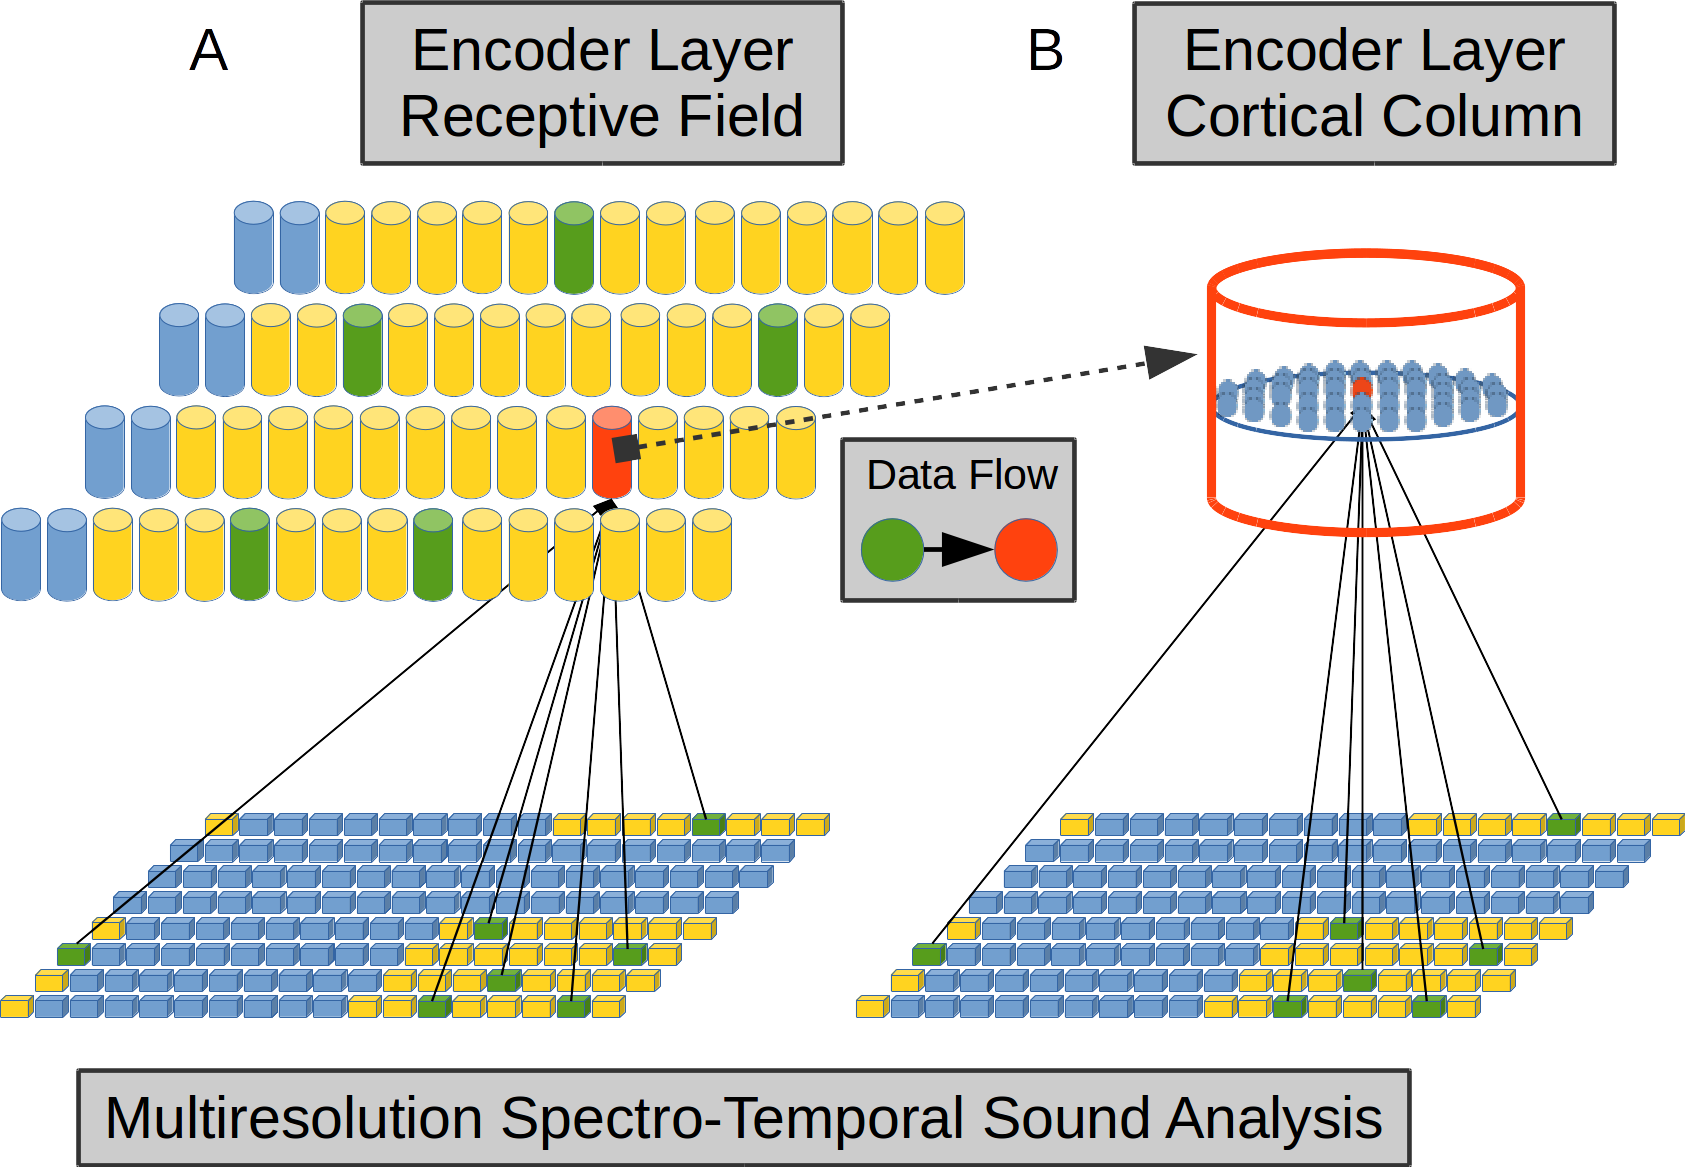
\includegraphics[width=0.8\textwidth]{EncoderProximalConnections.png}
    \caption{\glsfirst{el} proximal afferent connections. Each \gls{cc} in the \gls{el}--exemplified here in red--has its receptive field over the word2vec semantic space--in yellow.
    \textbf{(A)} A set of word2vec components--in green inside the receptive field--is randomly chosen to be connected with a \gls{cc}.
    \textbf{(B)} Each neural unit in a \gls{cc} is connected with the same set of word2vec components. We based this connectivity configuration on the vertical-orientation and on the prominent intra-columnar configuration of afferent axons received from layer IV.
    Adapted from https://doi.org/10.1371/journal.pone.0217966 under CC-BY license.}
    \label{fig:EncoderProximalConnections}
\end{figure}

The use of a \gls{som} per \gls{cc} in our model accounts for 
proximal lateral intra-column interaction, \gls{ltp}, \gls{ltd} and
the vertical organization of cell bands with similar response properties \cite{mountcastle_1955,Haueis2016}.
In each \gls{cc} in our model, clusters of neural units responding to similar semantic constraints emerge spontaneously from learning.
This has a correlate with the \emph{tonotopic}, \emph{retinotopic} or \emph{somatotopic} organization in brain tissue.
With such mechanism we also account for the \emph{full set of orientation columns and left and right ocular dominance} presented by \cite{doi:10.1002/cne.901580305} which we functionally simulate from a semantic information processing point of view.
In our modelling approach we account for the concept of cortical column as an \emph{elementary unit of organization} of the entire cerebral cortex \cite{doi:10.1152/jn.1957.20.4.408,Mountcastle1978AnOP,10.1093/brain/120.4.701}.

Figs. \ref{fig:CorticalColumnSOM} and \ref{fig:CorticalColumnTrainedSOM} show the relationship between the word2vec \gls{ds} space and each \gls{cc} in the \gls{el}.
In Fig. \ref{fig:CorticalColumnSOM} the \gls{cc} afferent dendrite is in its initial state and its corresponding semantic sub-space sampled from word2vec is represented by several words scattered in the background.
 
\begin{figure}[ht!]
    \centering
    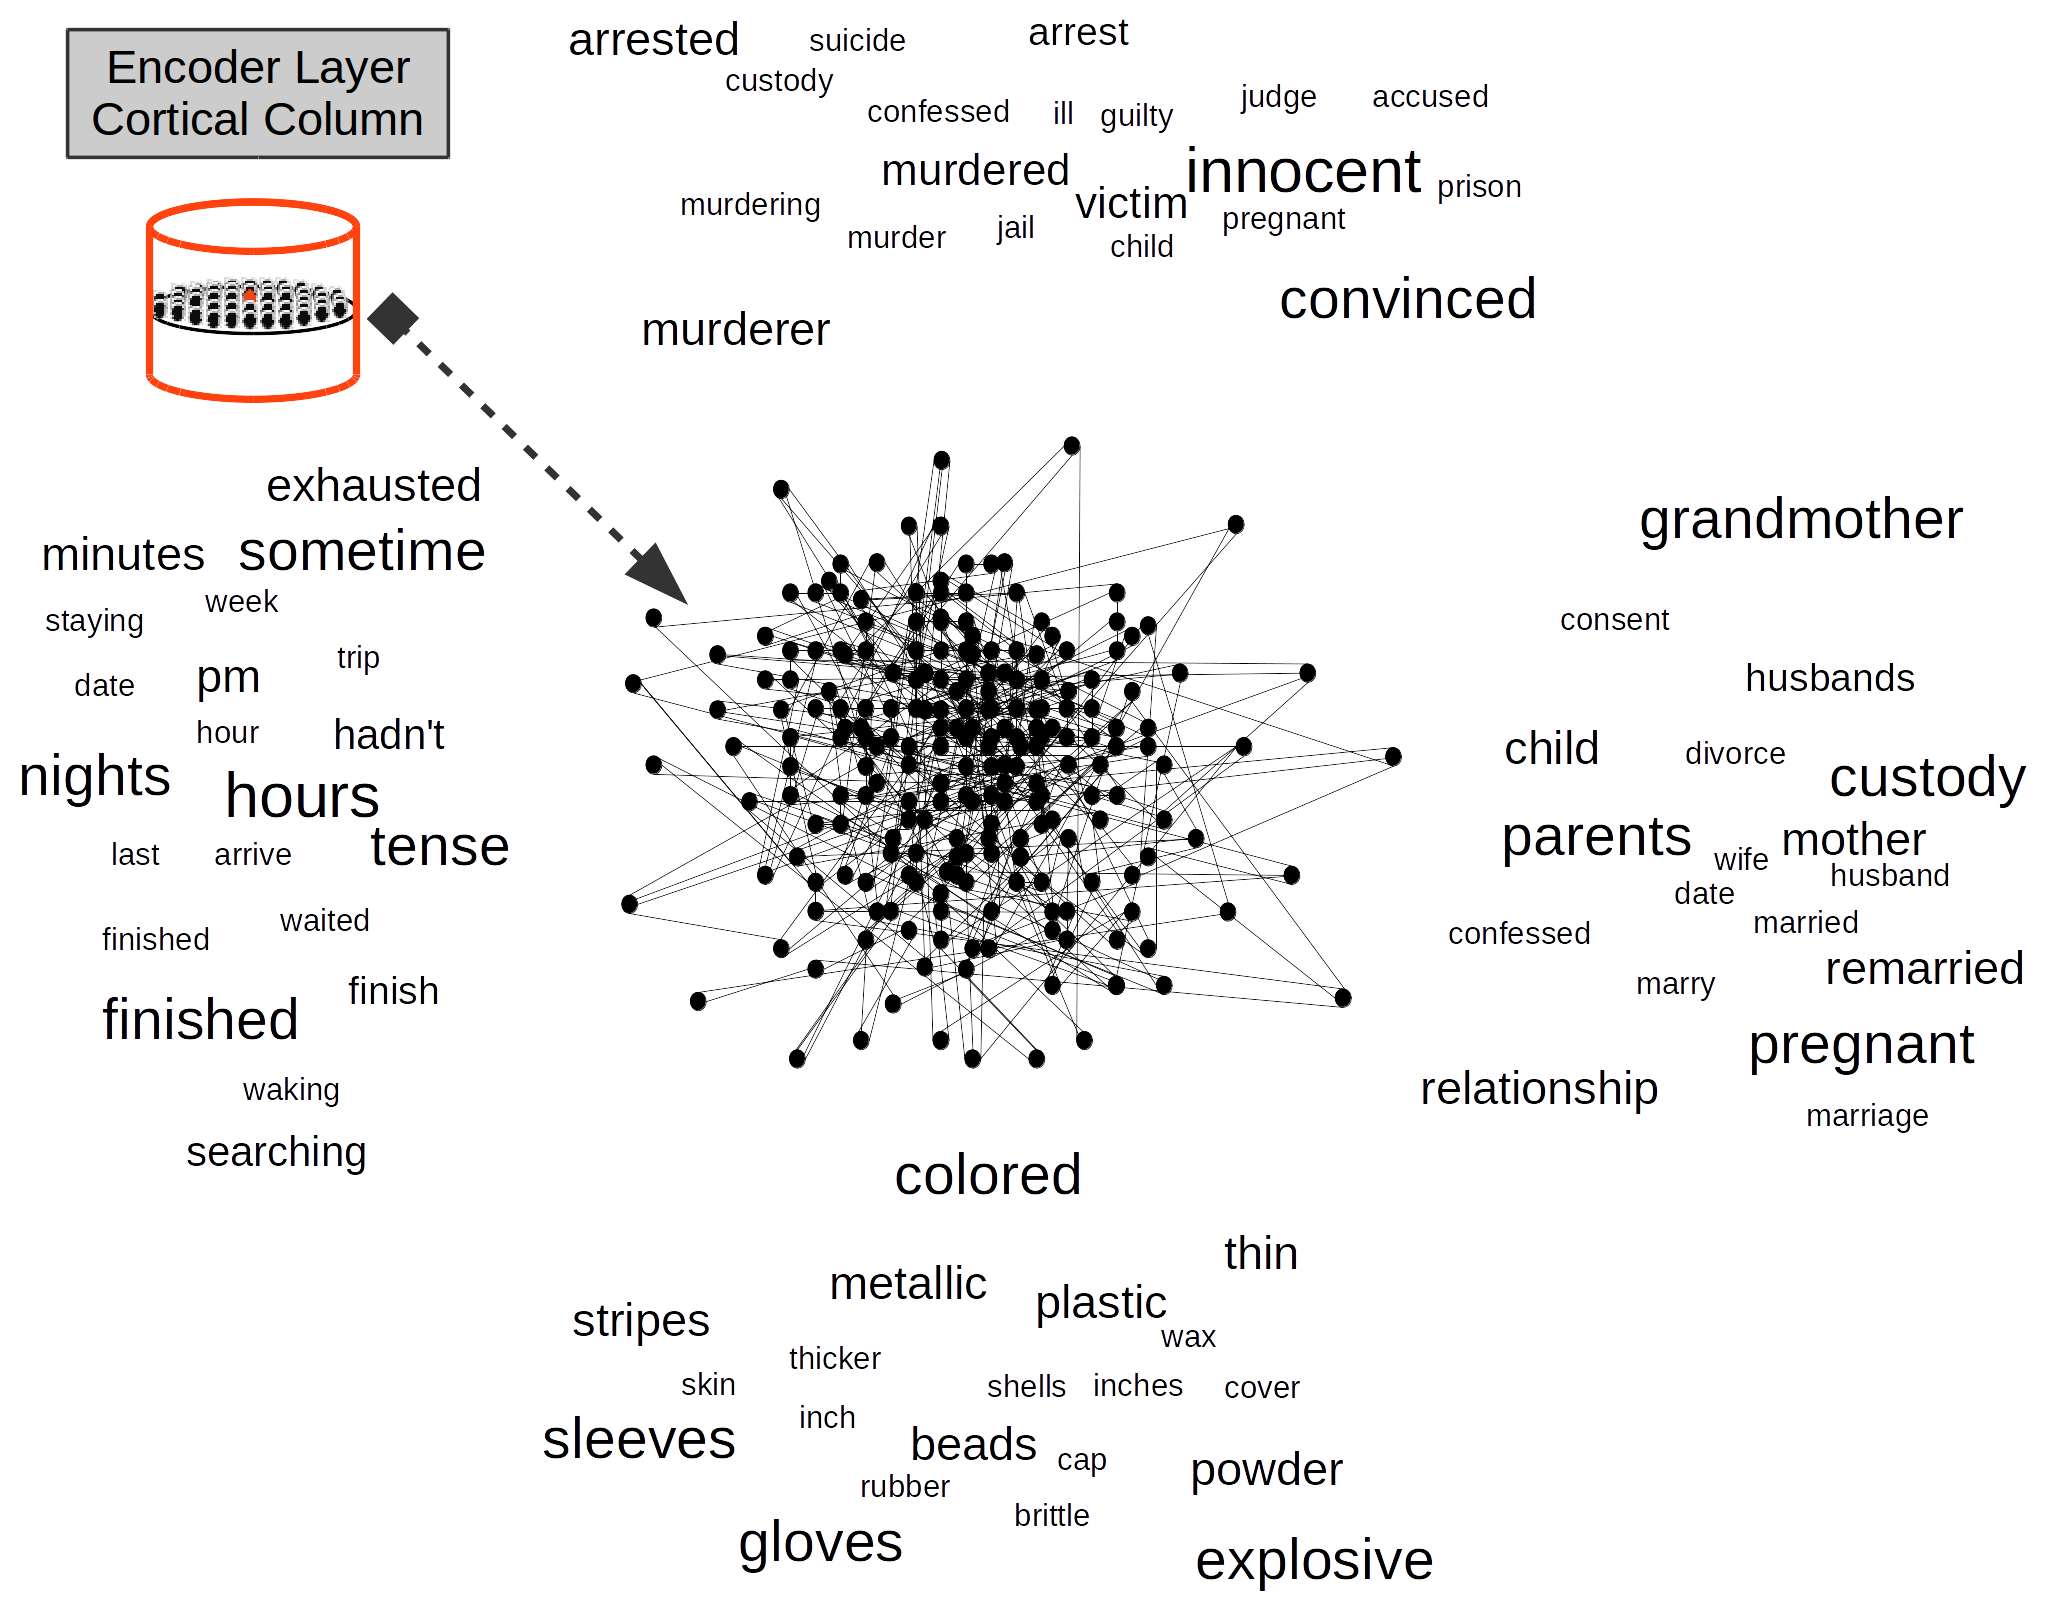
\includegraphics[width=0.8\textwidth]{CorticalColumnSOM.png}
    \caption{\glsfirst{el} \glsfirst{cc} and its proximal afferent dendrite whose synapses are simulated by a \glsfirst{som}. Each \gls{cc} in the \gls{el}--exemplified here in red--has its receptive field over word2vec as a semantic sub-space represented by words scattered in the background. \gls{som} weights are in their initial state. Adapted from https://doi.org/10.1371/journal.pone.0217966 under CC-BY license.}
    \label{fig:CorticalColumnSOM}
\end{figure}

Each set of afferent connections in a \gls{cc} determines a two-dimensional lattice of 15 by 15 neural units. The sampled semantic sub-space has 31 real valued components.
In Fig. \ref{fig:CorticalColumnTrainedSOM}--once the \gls{cc} afferent dendrite has been trained--the neural lattice distributes its neural units throughout the semantic sub-space. In such case, each word in the semantic sub-space will have its neural resource representation and words with semantic proximity in the semantic sub-space will be represented by neural resources with physical proximity in the lattice. The neighborhood preservation of self-organizing feature maps is an important property which turns out to be useful to preserve the original sub-space semantic relationships in the new space in the lattice of a \gls{cc} in the cortex \cite{557663}. Yet, even more importantly, the \gls{ds} remapping from word2vec subspace to the reduced dimensionality of the neural lattice reveals hidden relationships among the terms in the original sub-space as is the case in \gls{lsa} \cite{key:article}.

\begin{figure}[ht!]
    \centering
    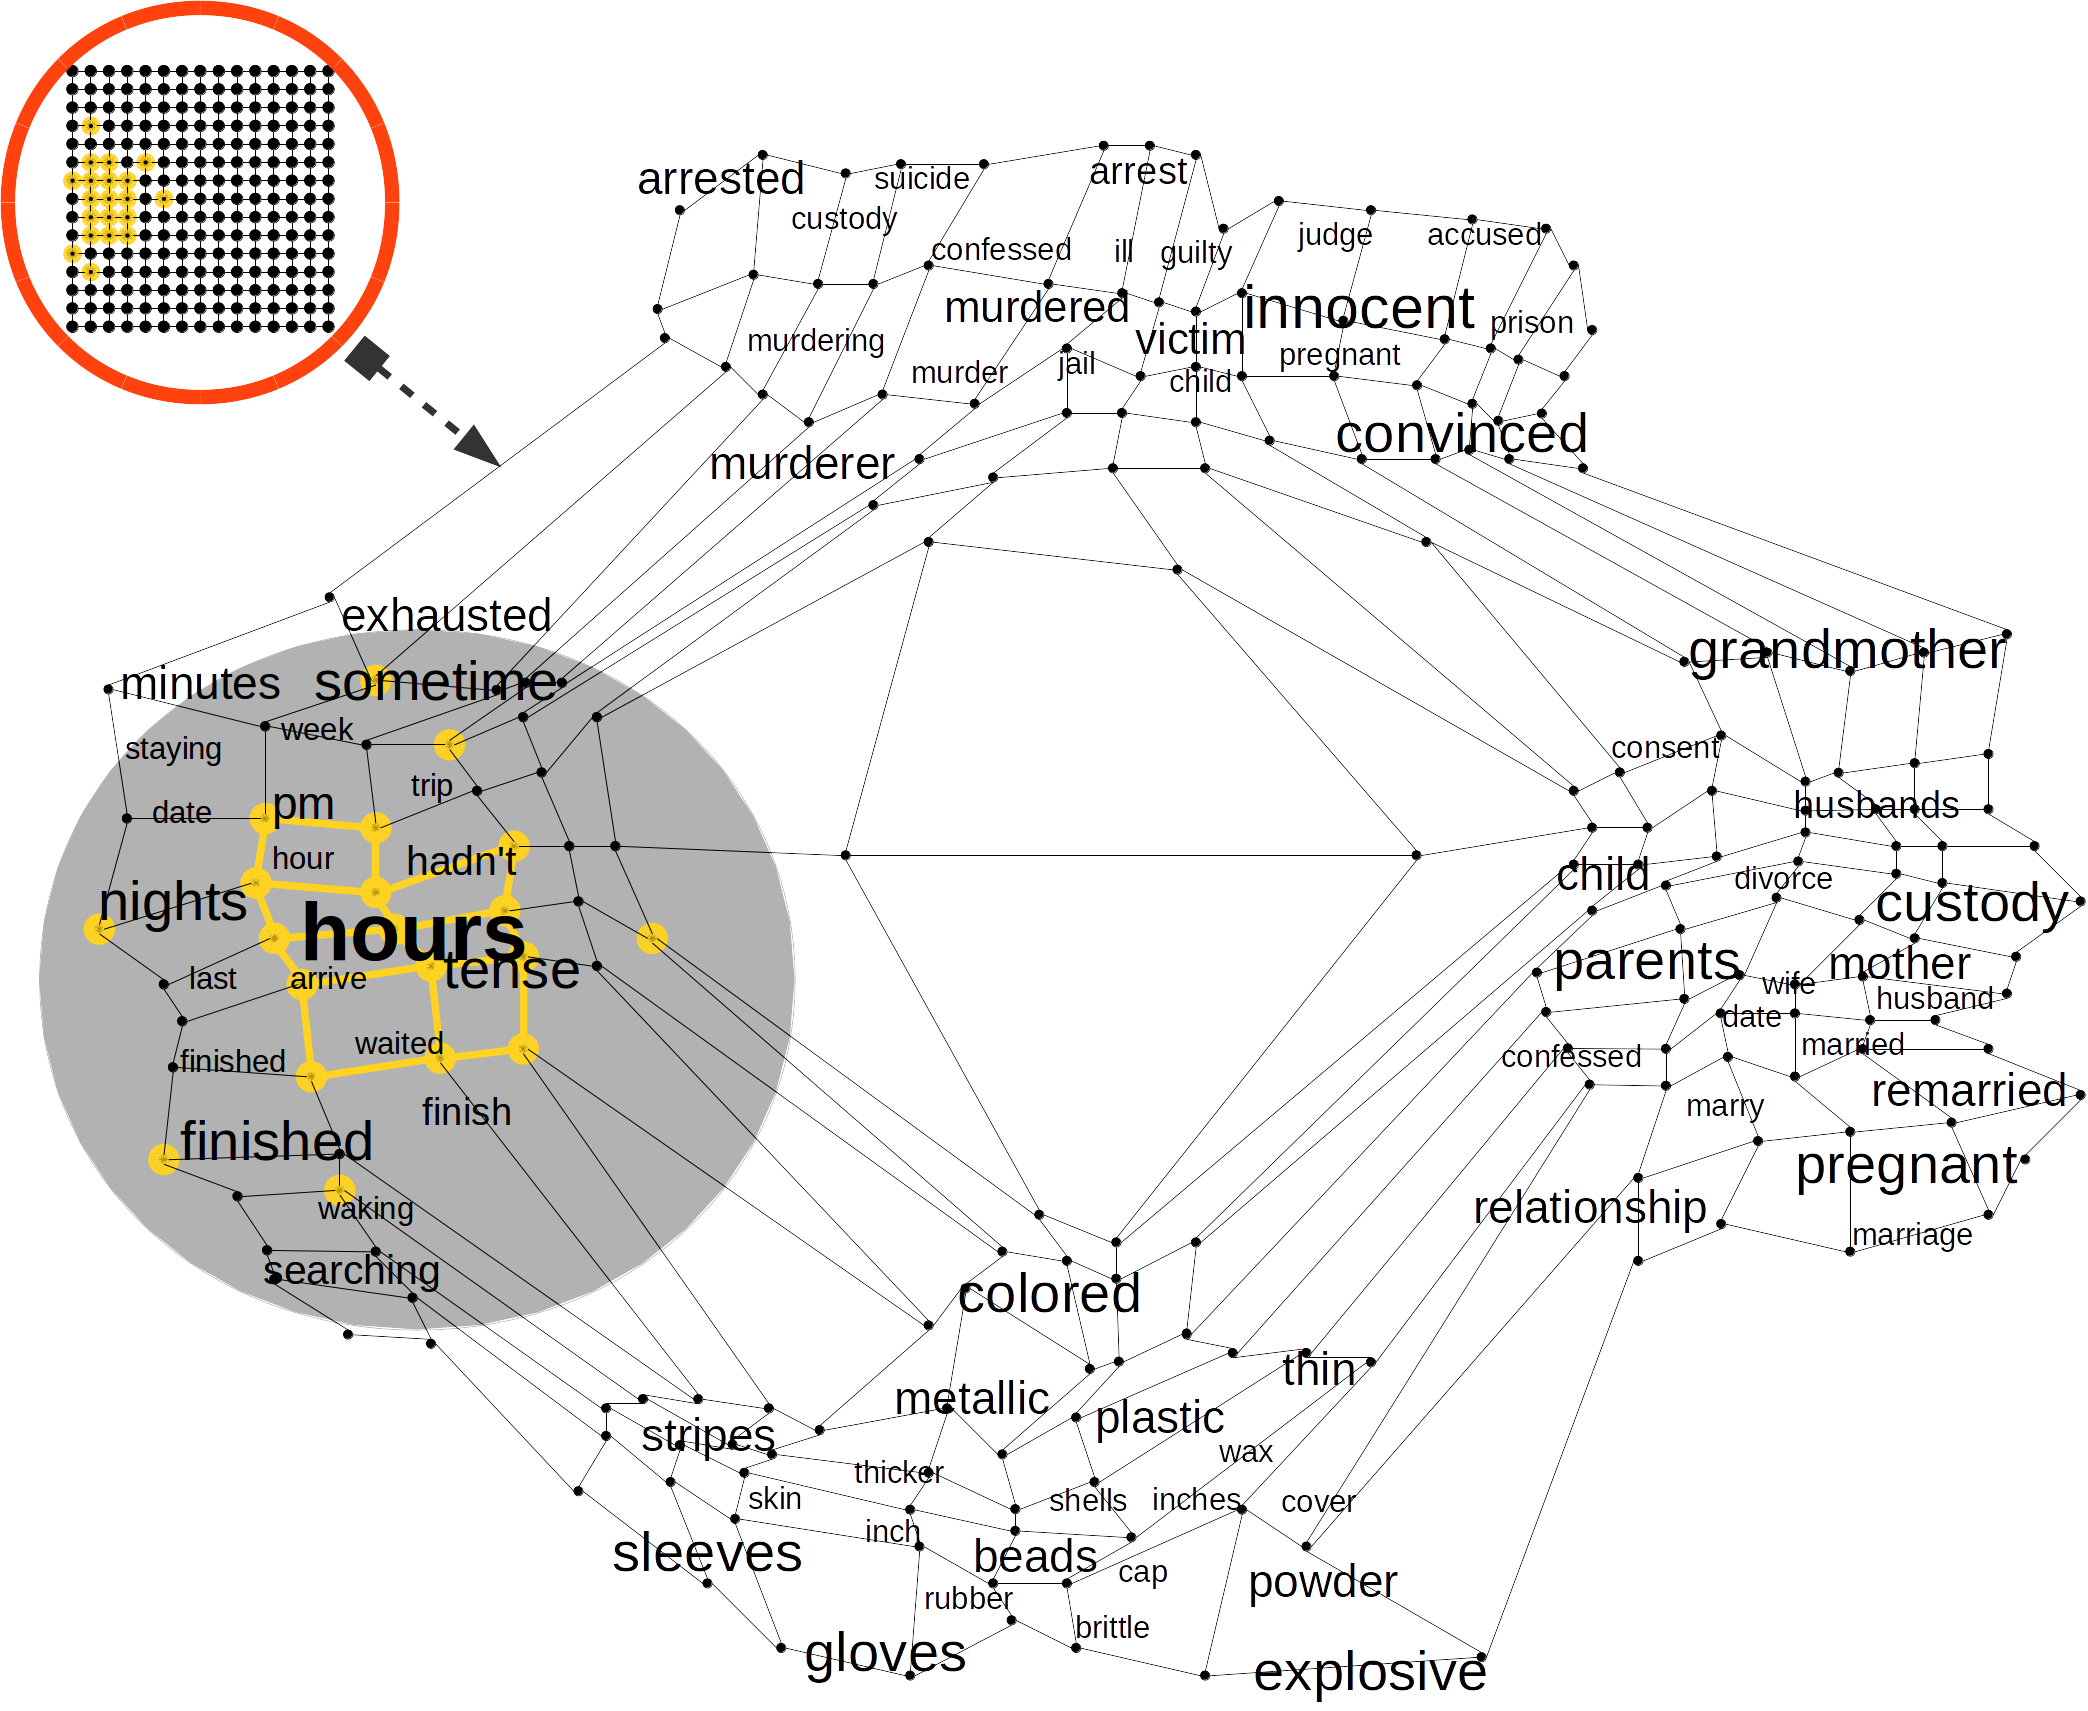
\includegraphics[width=0.8\textwidth]{CorticalColumnTrainedSOM.png}
    \caption{A trained \glsfirst{som} in a \glsfirst{cc} proximal afferent connections. The \gls{som} is a bi-dimensional lattice of 225 neural units (15 by 15 neural units). The \gls{som} adapts to represent the word2vec \glsfirst{ds} sub-space. After trained, a \gls{som} in a \gls{cc} distributes its neural units throughout the \gls{ds} sub-space sampled from word2vec. The \gls{som} algorithm keeps the semantic topology of the original \gls{ds} sub-space imprinted in the lattice of neural units. Each word in the \gls{ds} sub-space has its neural representation and words with more semantic similarity are represented by neural units with a high physical proximity in the lattice.}
    \label{fig:CorticalColumnTrainedSOM}
\end{figure}

Once afferent dendrites have learned the statistical distribution immersed in the different \glsfirst{ds} sub-spaces, each \gls{cc} in the \gls{el} has its private representation of its \gls{ds} sub-space from word2vec. The advent of the \gls{ds} representation from certain word in word2vec establishes a pattern of activation in a cluster of neural units inside each \gls{cc} (Fig. \ref{fig:CorticalColumnTrainedSOM}). In this way, each \gls{ds} constraint from word2vec will be represented in a distributed way throughout the \gls{el}. The semantic representation of each word will activate a cluster of neural units in each \gls{cc}, and the \gls{ds} content of such word will be distributed in the cortical patch simulated by the \gls{el}. Significant evidence shows that the semantic content of words is distributed across cortical tissue \cite{huth_natural_2016}. For example, a word like \emph{top} can not only activate a region related with clothing and appearance, but it can also activate a region related with numbers and measurements and perhaps a region related with buildings and places. On the other hand, it has also been shown that words with similar semantic content are mapped in proximal regions of the cortex \cite{pub.1005704802}. For instance, in the right temporo-parietal junction a small patch of cortex responds to words like \emph{wife, mother, pregnant, family, friends, brother} etc, while a very near patch responds to words like \emph{family} and \emph{wife} but also responds to--in certain way semantically related--words like \emph{house, roommates, household} and \emph{owner}. There are compelling brain-inspired computational approaches which use \glspl{sdr} to simulate how cortical brain activation represents the \glsfirst{ds} content of words \cite{DBLP:journals/corr/Webber15}.

In Fig. \ref{fig:CorticalColumnTrainedSOM} we illustrate how the word \textbf{\texttt{hours}} could activate a cluster of neural units which are representative of time phenomena such as \texttt{pm, hour} and \texttt{sometime}, but it could also  activate units which represent semantically related phenomena such as \texttt{tense}, which has to do with the form of a verb showing the time at which an action occurred, or the words \texttt{arrive, waiting} and \texttt{finished}, which are also--more indirectly--related with time.
Each \gls{cc} in our approach has a representative model of the \gls{ds} space and every column in the \gls{el} learns a complete model of such semantic representation. We rely on compelling brain-inspired computational theories in which every column in every region learns complete models of objects \cite{10.3389/fncir.2018.00121}.  

One important property to highlight in Fig. \ref{fig:CorticalColumnTrainedSOM} is that the advent of a word and its consequent semantic activation from word2vec will not determine a neural unit to fire, instead, it will bias the probability of such neural unit in doing so.
That is, the more excited a neural unit is by its afferent dendrite, the more likely it is that such unit will become active. That is why neural units which are closer to the active word vector in the sub-space will tend to be more densely active than neural units farther apart, as Fig. \ref{fig:CorticalColumnTrainedSOM} shows. The stochastic behavior of cells in neural tissue is a widely used property not only in bio-inspired models \cite{harrison_l.m_stochastic_2005} but also in \glspl{ann} such as \gls{dl} networks by means of techniques like dropout~\cite{Srivastava2014DropoutAS} which is used to reduce unwanted phenomena such as overfitting.
}








\iftoggle{DEBUG}{
\subsection{Restricciones Secuenciales Laterales y Sintácticas Gruesas}

Es generalmente aceptado que--a diferencia de las células en la capa IV que responden a estímulos más simples--las células de las capas II/III se conocen como \emph{células complejas} que reaccionan a movimientos o células que responden a diferentes realizaciones de la misma característica de manera invariante \cite{10.1371/journal.pcbi.1000532}.
Por ejemplo, células en las capas II/III en áreas corticales visuales favorecen--en gran medida--a estímulos más ricos, tales como movimientos en direcciones preferidas \cite{HIRSCH2006377}.
Esto es consistente con nuestra propuesta de que las células de las capas II/III representan diferentes patrones en el contexto de diferentes secuencias.
Las neuronas se activan de acuerdo al contexto en la secuencia correcta.

Las dendritas distales en cada unidad neuronal en la \gls{el} se clasifican en dos grupos: (i) dendritas laterales que  conectan una \gls{cc}--en color rojo en la Fig. \ref{fig:DistalDendrites1} A--con dendritas en \gls{cc_pl} vecinas en el mismo parche cortical--en color verde en la \gls{el} en la Fig. \ref{fig:DistalDendrites1} A.
Se conoce que los axones de las neuronas piramidales en las capas II/III viajan varios milímetros paralelamente a las capas II/III y/o los límites de la capa IV ingresando nuevamente en las capas II/III para realizar conexiones excitatorias con células piramidales allí \cite{BANNISTER200595,10.1093/cercor/13.1.15}.
Luego (ii) las dendritas apicales; las cuales vinculan una \gls{cc} en la \gls{el} a \gls{cc_pl} en otro parche cortical.
En este trabajo las dendritas apicales traen información desde un \glsfirst{rf} que establece restricciones sintácticas gruesas en el sistema--Fig. \ref{fig:DistalDendrites1} A.

\begin{figure}[ht!]
    \centering
    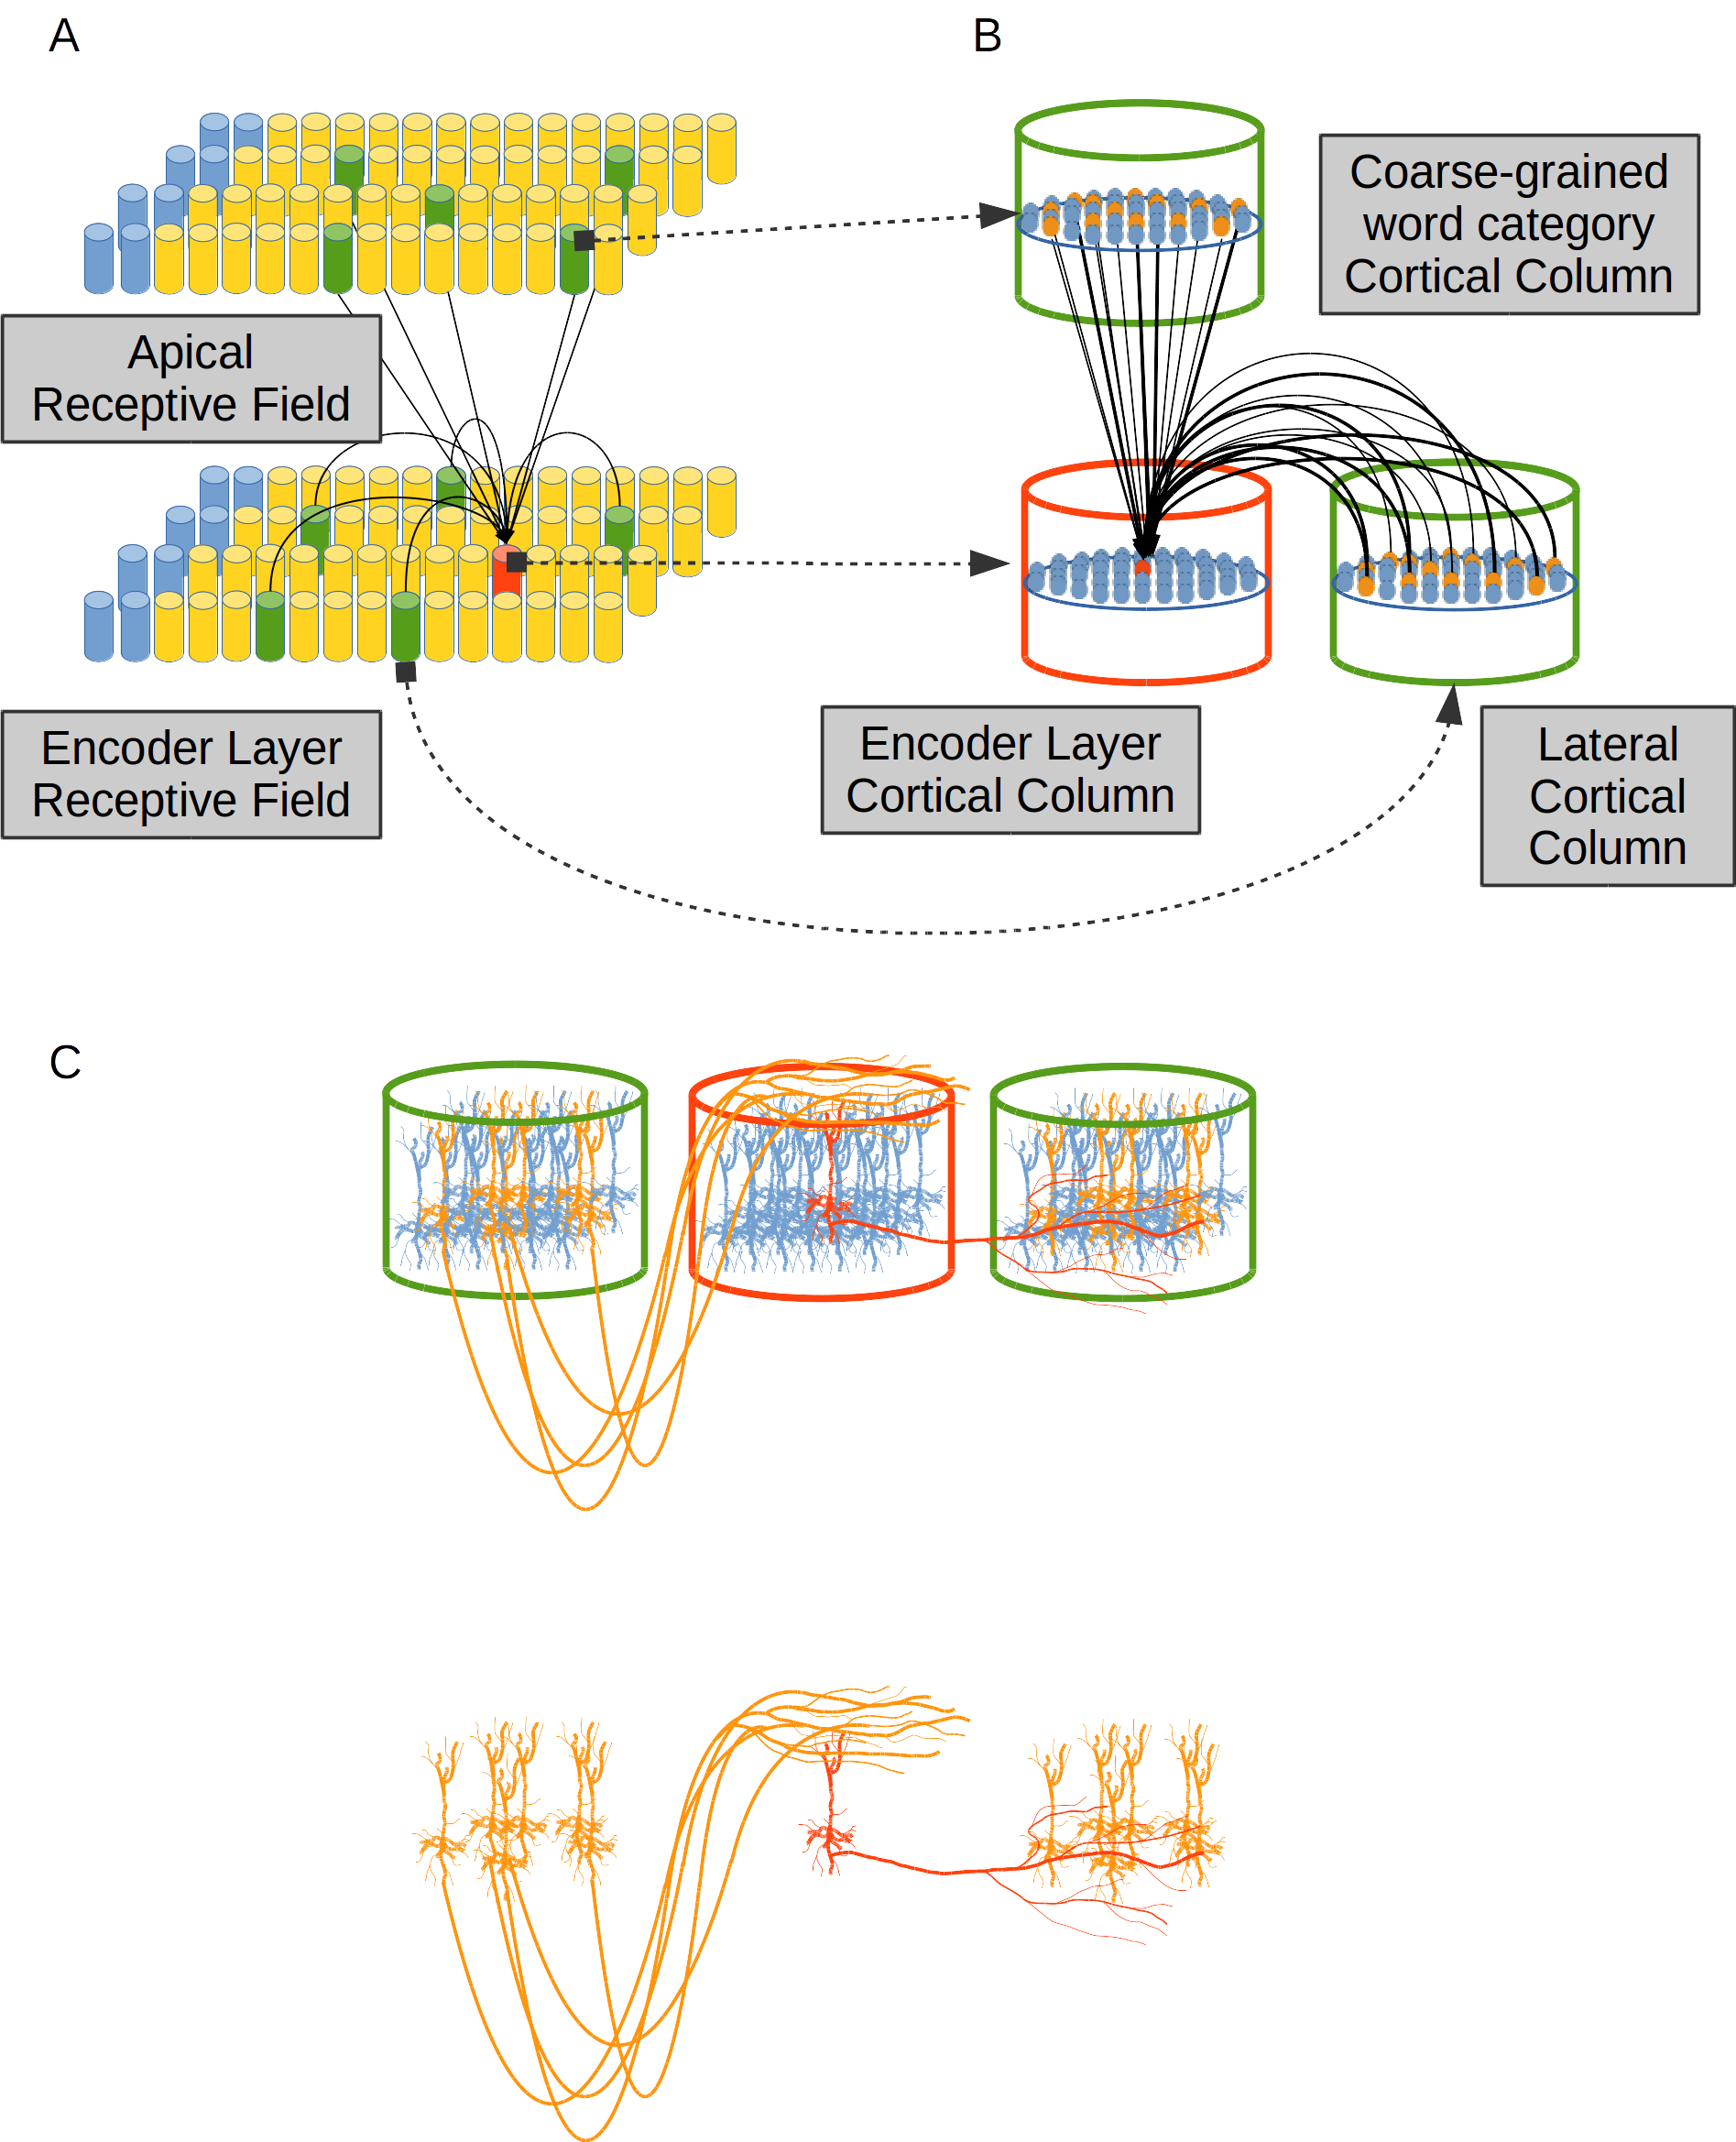
\includegraphics[width=0.8\textwidth]{DistalDendrites1.png}
    \caption{Dendritas distales en la \gls{el}.
	    \textbf{(A)} Las dendritas distales pueden ser (i) laterales, vinculando \gls{cc_pl} vecinas en el mismo parche cortical, y (ii) apicales, las cuales vinculan \gls{cc_pl} en parches corticales diferentes.
	    \textbf{(B)} Una rama dendrítica  distal entre la \gls{cc} de color rojo y una \gls{cc} verde significa que cada unidad neuronal en la \gls{cc} roja se vincula con un sub-conjunto diferente de unidades neuronales en la \gls{cc} verde por medio de conexiones potenciales. El subconjunto de conexiones potenciales viene de un porcentaje de unidades neuronales dentro de la \gls{cc} verde. Tal porcentaje es un parámetro ajustable para la \gls{cc}.
    \textbf{(C)} La proximidad física de una rama dendrítica desde una célula roja a ramas axonales desde células amarillas determinan conexiones potenciales que pueden prosperar convirtiéndose en sinapsis establecidas dependiendo de la actividad entre las células.
    Imagen adaptada de \url{https://doi.org/10.1371/journal.pone.0217966 bajo licencia CC-BY}.}
    \label{fig:DistalDendrites1}
\end{figure}

Una dendrita distal vinculando dos \gls{cc_pl} como en la Fig. \ref{fig:DistalDendrites1} A implica que cada unidad neuronal en una \gls{cc}--en color rojo en la Fig. \ref{fig:DistalDendrites1} B--se vincula con un subconjunto de unidades en \gls{cc_pl} vecinas en el mismo parche cortical, o en otras \gls{cc_pl} en parches corticales foráneos, como se muestra en color verde en la Fig. \ref{fig:DistalDendrites1} B.
Tal subconjunto de unidades neuronales es determinado por las configuraciones físicas anatómicas de las dendritas desde una unidad neuronal roja en la Fig. \ref{fig:DistalDendrites1} B a unidades neuronales amarillas en las \gls{cc_pl} verdes, como se muestra en la Fig. \ref{fig:DistalDendrites1} C.

La Fig. \ref{fig:DistalDendrites1} C muestra cómo las dendritas laterales se extienden a través de la corteza para vincular una unidad neuronal a otras unidades neuronales en \gls{cc_pl} vecinas en el mismo área cortical--la \gls{el} en nuestro caso.
Las dendritas apicales, por otro lado, reciben información desde \gls{cc_pl} ubicadas en parches corticales foráneos por medio de axones extendidos que dejan sus dominios corticales, viajan a través de la sustancia blanca y finalmente ingresando en el área cortical \gls{el} hasta la capa más superficial de la corteza llamada L1, donde se extienden dendritas apicales desde células locales. 


La Fig. \ref{fig:DistalDendritesGrowth} ilustra el proceso de crecimiento sináptico en las dendritas distales. 
El recuadro rojo representa una \gls{cc} cuyas ramas dendríticas distales vinculan sus unidades neuronales en otras \gls{cc_pl} en verde en la figura.

\begin{figure}[ht!]
    \centering
    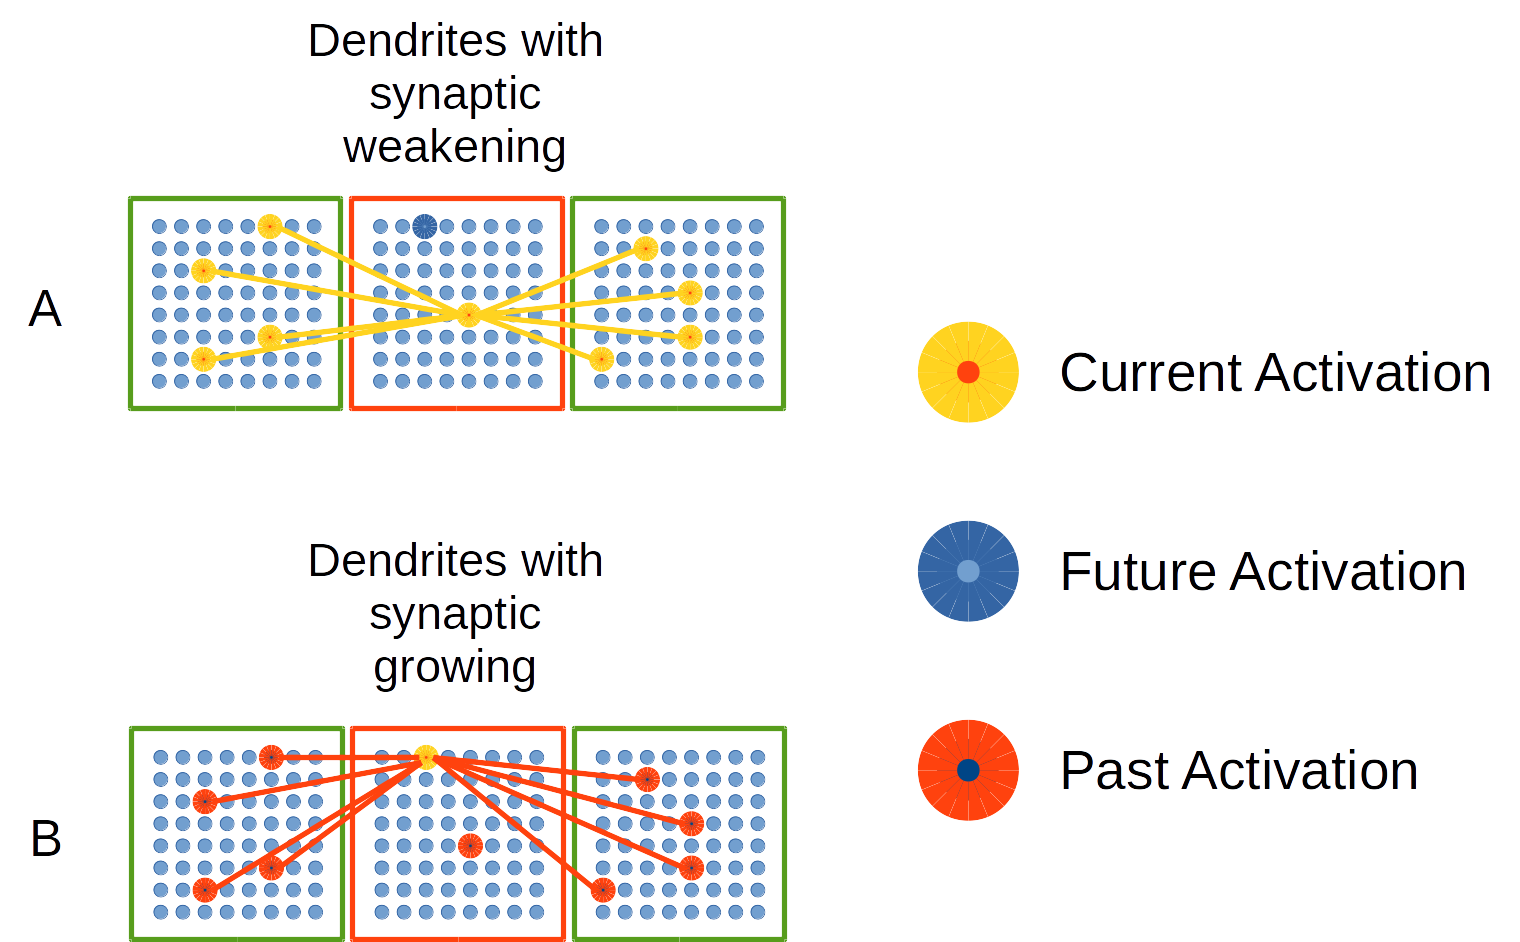
\includegraphics[width=0.8\textwidth]{DistalDendritesGrowth.png}
    \caption{Crecimiento Sináptico en dendritas distales en la \gls{el}.
    Imagen adaptada de \url{https://doi.org/10.1371/journal.pone.0217966} bajo licencia CC-BY.}
    \label{fig:DistalDendritesGrowth}
\end{figure}

En la Fig. \ref{fig:DistalDendritesGrowth} A, la activación actual y simultánea de unidades neuronales en \gls{cc_pl} vinculadas, decrementa el peso sináptico en las sinapsis potenciales en tales dendritas.
En la Fig. \ref{fig:DistalDendritesGrowth} B, se refuerzan las sinápsis potenciales entre neuronas activadas ahora y activadas en el pasado.
Este mecanismo de crecimiento sináptico simula el proceso biológico de \glsfirst{stdp} en la corteza.
 
Como ya ha sido mencionado, las dendritas laterales traen información desde la actividad previa en \gls{cc_pl} vecinas en la \gls{el}.
Esto agrega restricciones a la activación de unidades neuronales en relación a la activación previa en el mismo área cortical.
De esta forma se producirían restricciones sintácticas las que sesgarían la activación de ciertos patrones en comparación con otros menos coherentes en relación a las regularidades secuenciales estadísticas inmersas en la estructura gramatical de los estímulos.

Las dendritas apicales traen información desde parches corticales foráneos.
Para proveer tal información, generamos tres \gls{sdr_pl} que proveen un indicio grosero a la \gls{el} acerca de tres categorías principales de palabras: (i) palabras de contenido, (ii) palabras de función, y desde el conjunto de palabras de contenido segregamos los (iii) verbos.
Investigaciones previas han mostrado que la distinción entre palabras de contenido/función se encuentra marcada acústicamente, fonológicamente y distribucionalmente en el habla que los infantes oyen en diferentes lenguajes \cite{Shi1995PerceptualCO,shi_morgan_allopenna_1998}.
Aún infantes recién nacidos pueden discriminar clases de palabras categoricamente basados solamente en pistas acústicas y fonológicas.
Es más, las pistas fonológicas pueden ayudar a infantes de más edad en la adquisición de categorías gramaticales y estructura sintáctica \cite{shi_newborn_1999}.
Se ha mostrado empíricamente que la conversión sustantivo-verbo se puede determinar por medio de propiedades fonológicas de las clases de palabras \cite{lohmann_phonological_2017}.
En tal aspecto, las pistas fonológicas se pueden emplear para palabras de al menos dos sílabas para la determinación de la direccionalidad de la conversión sustantivo-verbo.
Consideramos que las restricciones fonológicas podrían proveer un repertorio mucho más rico y detallado, pero mantenemos tales restricciones al mínimo para probar la reacción del modelo utilizando la mínima información que la fonología podría proveer.
}{
\subsection{Lateral Sequential and Apical Coarse-Grained Syntactic Constraints}

It is generally believed that--unlike cells in layer IV that respond to more shallow stimuli--cells in layer II/III are known to be \emph{complex cells} that respond to sequence of motion or cells that respond to different translations of the same feature in an invariant way \cite{10.1371/journal.pcbi.1000532}.
For instance, cells in layer II/III in visual and barrel cortical areas--to a great extent--favour richer stimuli, such as motion in the preferred direction \cite{HIRSCH2006377}. This is consistent with our proposal that layer II/III cells represent different  patterns in the context of different sequences. They become active according to the context of the correct sequence.

Distal dendrites in each neural unit in the \gls{el} are classified in two sets: (i) lateral dendrites which connect a \gls{cc}--in red in Fig. \ref{fig:DistalDendrites1} A--to neighboring \glspl{cc} in the same cortical patch--in green in the \gls{el} in Fig. \ref{fig:DistalDendrites1} A.
It is known that layer II/III pyramidal neurons axons travel several millimeters parallel to the layer II/III and/or layer IV boundary re-entering in layer II/III to make excitatory connections to pyramidal cells there \cite{BANNISTER200595,10.1093/cercor/13.1.15}.
Then (ii) apical dendrites which link a \gls{cc} in the \gls{el} to \glspl{cc} in another cortical patch. In the present work, apical dendrites bring information from a \gls{rf} which establishes coarse-grained syntactic constraints in the system--Fig. \ref{fig:DistalDendrites1} A.

\begin{figure}[ht!]
    \centering
    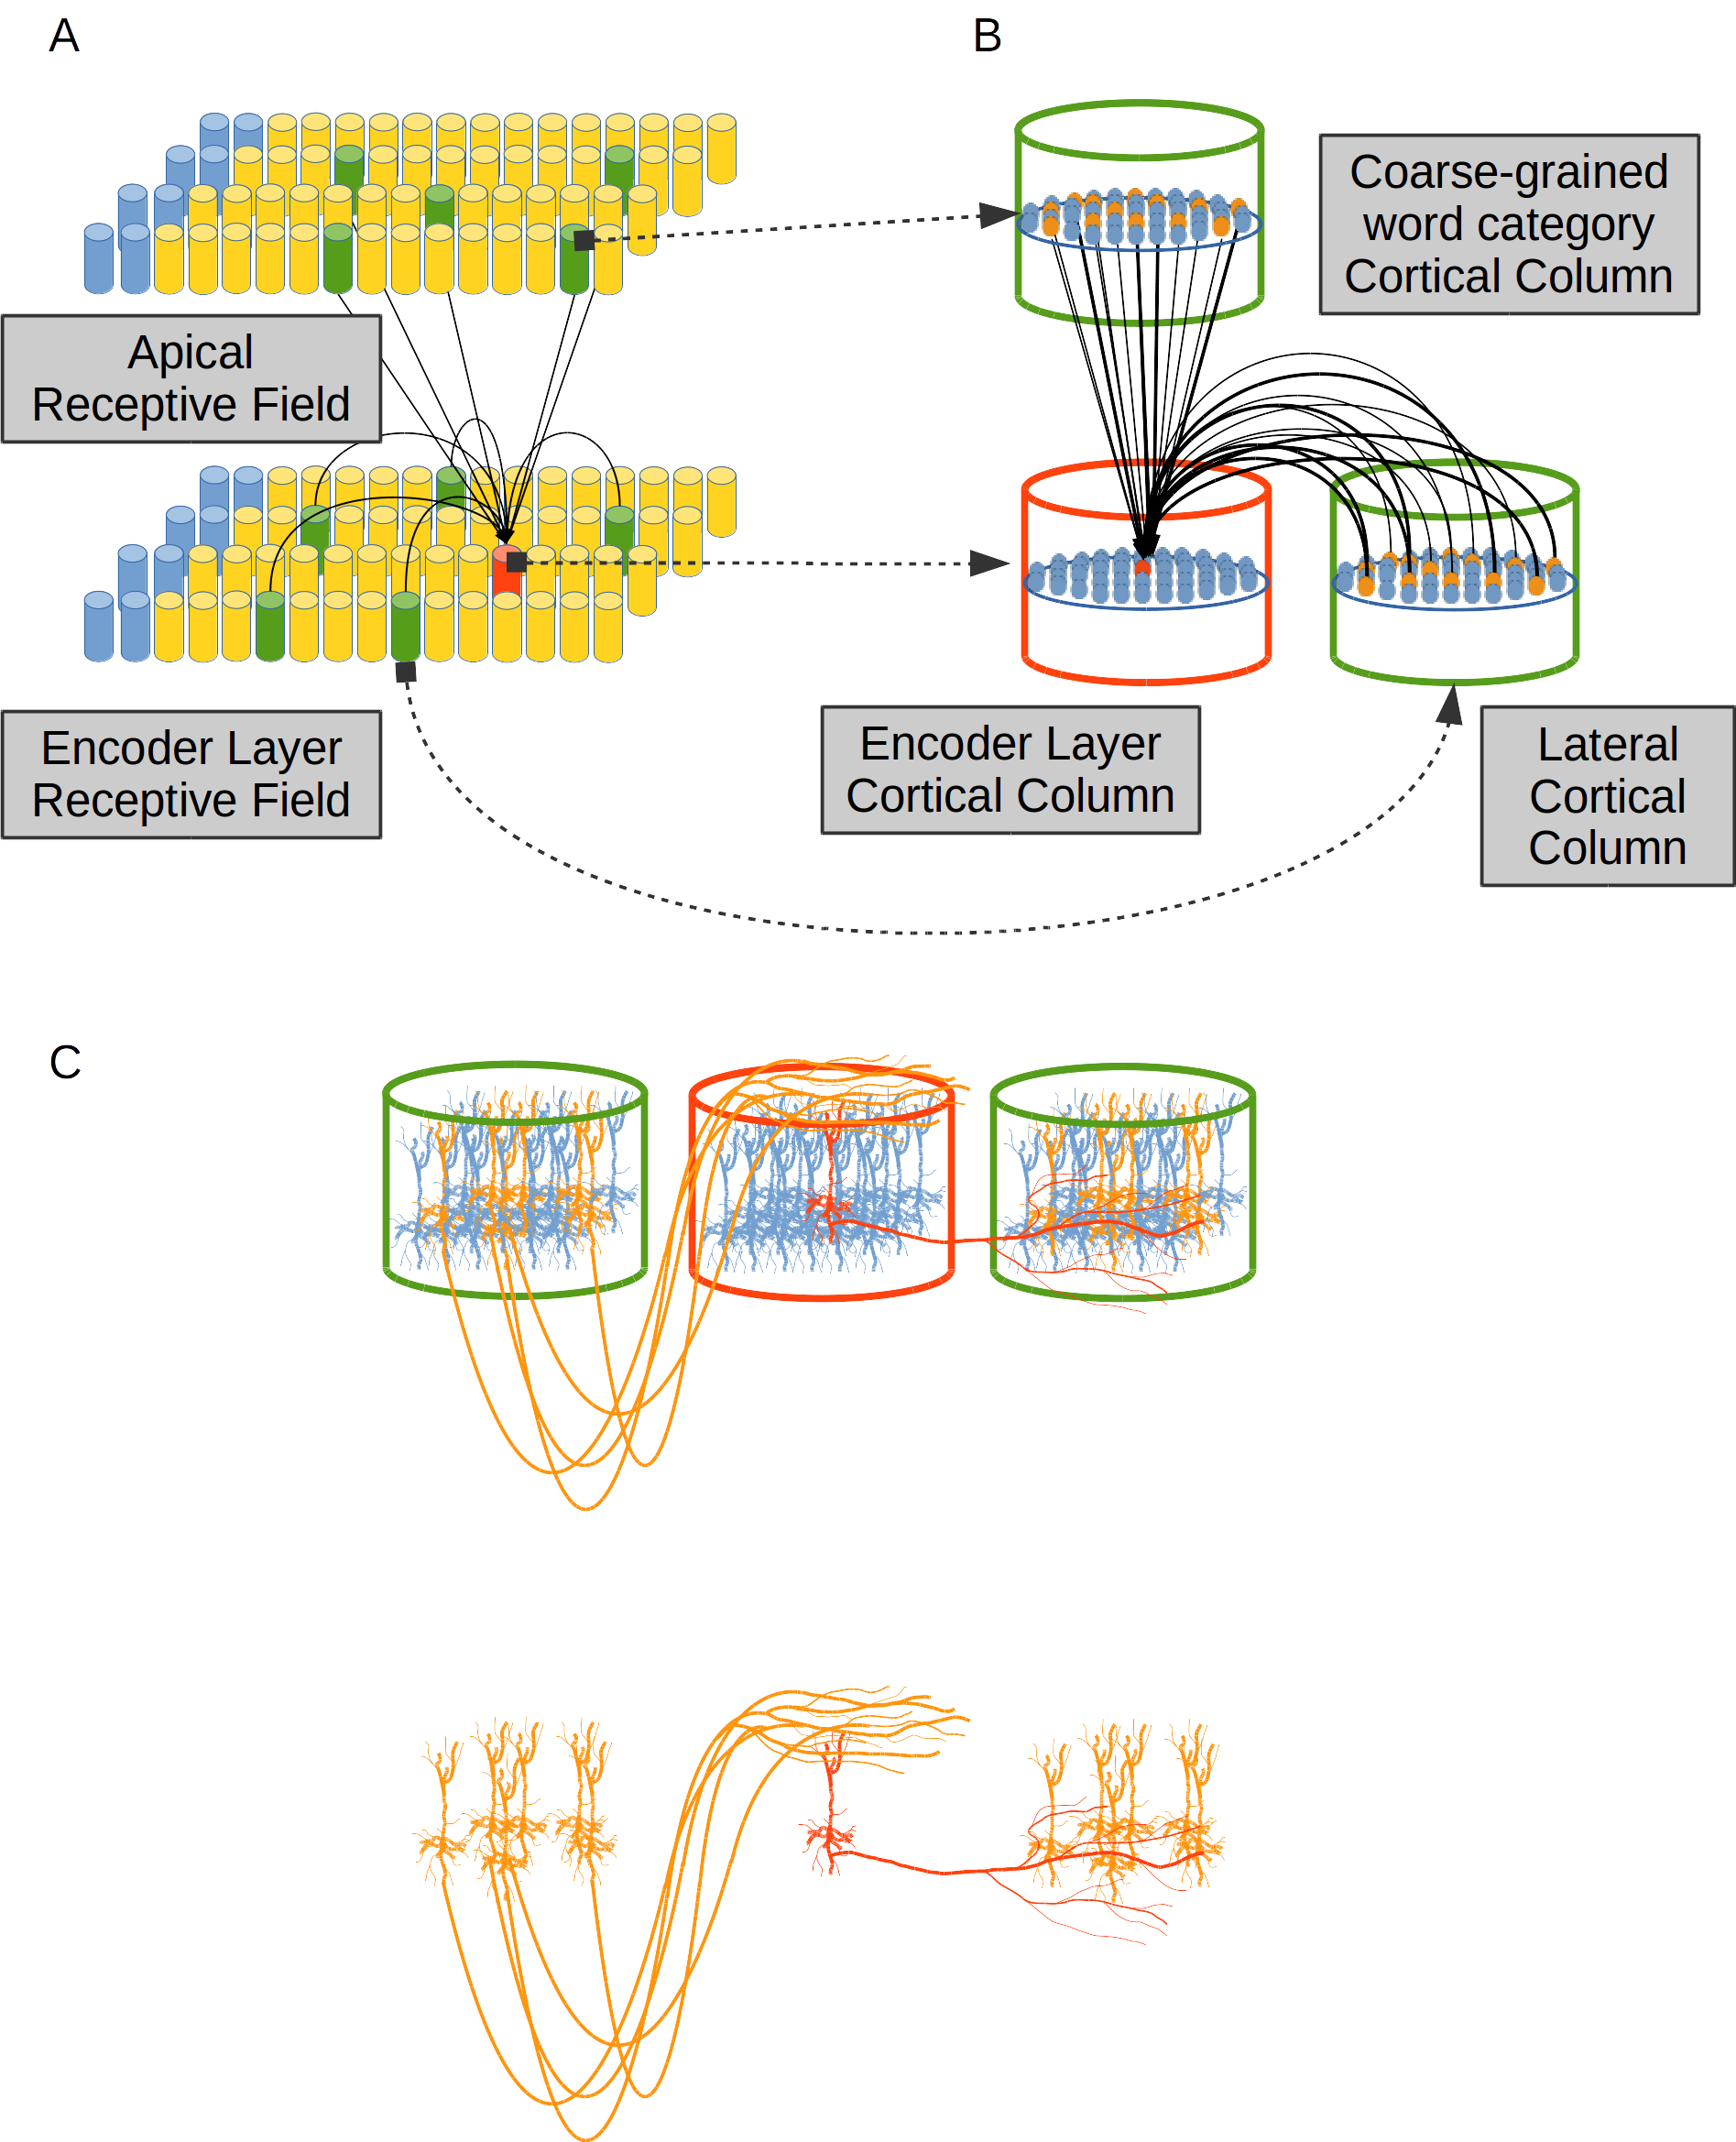
\includegraphics[width=0.8\textwidth]{DistalDendrites1.png}
    \caption{Distal dendrites in the \gls{el}.
    \textbf{(A)} Distal dendrites can be (i) lateral, linking neighboring \glspl{cc} in the same cortical patch, and (ii) apical, which link \glspl{cc} in different cortical patches.
    \textbf{(B)} A distal dendritic branch between the red \gls{cc} and a green \gls{cc} entails that every neural unit in the red \gls{cc} is linked to a different subset of neural units in the green \gls{cc} by means of potential connections. The subset of potential connections comes from a percentage of neural units inside the green \gls{cc}. Such percentage is a tunable parameter for the \gls{cc}.
    \textbf{(C)} Physical proximity of a dendritic branch from the red cell to axonal branches from yellow cells determines potential connections which could prosper becoming in established synapses depending on the activity among cells.
    Adapted from \url{https://doi.org/10.1371/journal.pone.0217966 under CC-BY license}.}
    \label{fig:DistalDendrites1}
\end{figure}

A distal dendrite linking two \glspl{cc} as in Fig. \ref{fig:DistalDendrites1} A implies that each neural unit in a \gls{cc}--in red in Fig. \ref{fig:DistalDendrites1} B--is linked to a sub-set of units in neighboring \glspl{cc} in the same cortical patch, or in other \glspl{cc} in a foreign cortical patch, as shown in green in Fig. \ref{fig:DistalDendrites1} B. Such sub-set of neural units is determined by the physical anatomical configurations of dendrites from the red neural unit in Fig. \ref{fig:DistalDendrites1} B to the yellow neural units in green \glspl{cc}, as shown in Fig. \ref{fig:DistalDendrites1} C.

Fig. \ref{fig:DistalDendrites1} C shows how lateral dendrites extend through cortex to link a neural unit to other neural units in neighboring \glspl{cc} in the same cortical patch--the \gls{el} in our case. Apical dendrites on the other hand, receive information from \glspl{cc} located in foreign cortical patches by means of extended axons which leave their cortical domain, travelling through white matter and finally entering the \gls{el} cortical patch up to the most superficial layer of cortex called L1, where apical dendrites from local cells extend.


Fig. \ref{fig:DistalDendritesGrowth} depicts the process of synaptic growth in distal dendrites. The red square represents a \gls{cc} whose distal dendritic branches link its neural units to neural units in other \glspl{cc} in green in the figure.

\begin{figure}[ht!]
    \centering
    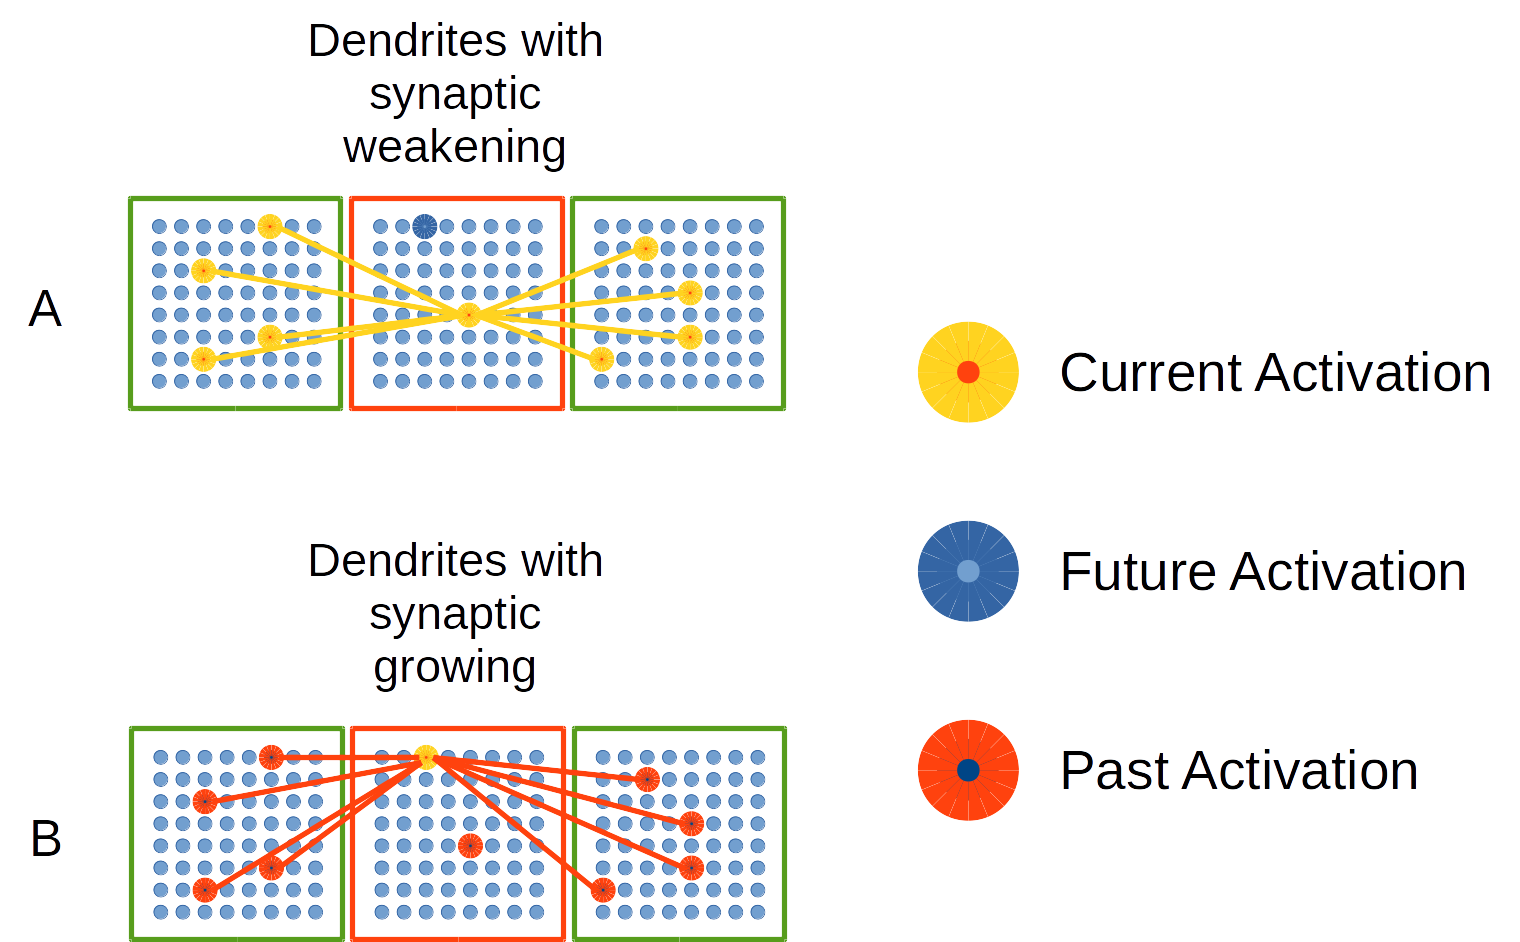
\includegraphics[width=0.8\textwidth]{DistalDendritesGrowth.png}
    \caption{Synaptic growth in distal dendrites in the \gls{el}.
    Adapted from \url{https://doi.org/10.1371/journal.pone.0217966} under CC-BY license.}
    \label{fig:DistalDendritesGrowth}
\end{figure}

 In Fig. \ref{fig:DistalDendritesGrowth} A, the current and simultaneous activation of neural units in linked \glspl{cc} decreases the synaptic strength in the potential synapses in such dendrites. In Fig. \ref{fig:DistalDendritesGrowth} B, potential synapses among currently activated neural units and past activated ones are strengthened. This mechanism of synaptic growth simulates \gls{stdp} biological processes in cortex.
 
 As already mentioned, lateral dendrites bring information from previous activity in neighboring \glspl{cc} in the \gls{el}. This adds restrictions to the activation of neural units regarding previous activation in the same area. This would produce syntactic constraints which would bias the activation of certain patterns compared to others which are less coherent regarding the statistical sequential regularities immerse in the grammatical structure of the stimuli.

Apical dendrites bring information from foreign cortical patches.
In order to provide such information, we generate three \glspl{sdr} which supply a coarse clue to the \gls{el} about three major word categories: (i) content words, (ii) function words and from content words we segregate (iii) verbs.
Previous research has shown that content-function word distinction is marked acoustically, phonologically, and distributionally in the speech infants hear in different languages \cite{Shi1995PerceptualCO,shi_morgan_allopenna_1998}.
Even newborn infants can categorically discriminate word classes based solely on acoustic and phonological cues.
Furthermore, such phonological cue can help older infants bootstrap into the acquisition of grammatical categories and syntactic structure \cite{shi_newborn_1999}.
\cite{lohmann_phonological_2017} empirically showed that noun-verb conversion can be determined via phonological properties of word class. In such regard, phonological cues can be employed for words of at least two syllables for the determination of the directionality of the noun-verb conversion.
We consider that phonological constraints could provide a much richer and fine-grained correlated repertoire, yet we kept such constraints at a minimum in order to test the model's reaction using the minimal hint phonology could provide.
}













\iftoggle{DEBUG}{
\subsection{Activación Cortical en la Capa Encoder}

La dinámica de la activación celular en la \gls{el} se muestra en la Fig. \ref{fig:Activation1}.
La correlación repetida entre restricciones de la \gls{ds} aferente, laterales secuenciales y apicales en categorías gruesas de palabras determina el peso de las sinapsis dendríticas de tal manera que ciertos eventos serán más predecibles que otros.
Mientras que la secuencia de constituyentes oracionales mantengan cierto nivel de predictibilidad con respecto al material de entrenamiento, los patrones de activación en la \gls{el} retornarán suficiente dispersión, y un fenómeno repetitivo de diferentes \gls{sdr_pl} será sostenido en el tiempo.
Cuando eventos impredecibles--con respecto al material de entrenamiento--surjan, la dispersión no puede ser sostenida por la red y un fenómeno llamado \glsfirst{mfe} emergerá como consecuencia de la incapacidad de la red para predecir correctamente tales eventos.
Como resultado de la ignorancia de la red para predecir correctamente un evento, esta activa todas las hipótesis más probables dadas las restricciones semánticas.
Des esta forma, la \gls{el} pierde el sesgo establecido por las restricciones sintácticas, abriendo la puerta a más hipótesis para recibir eventos léxicos subsecuentes en mejores condiciones.

\begin{figure}[ht!]
    \centering
    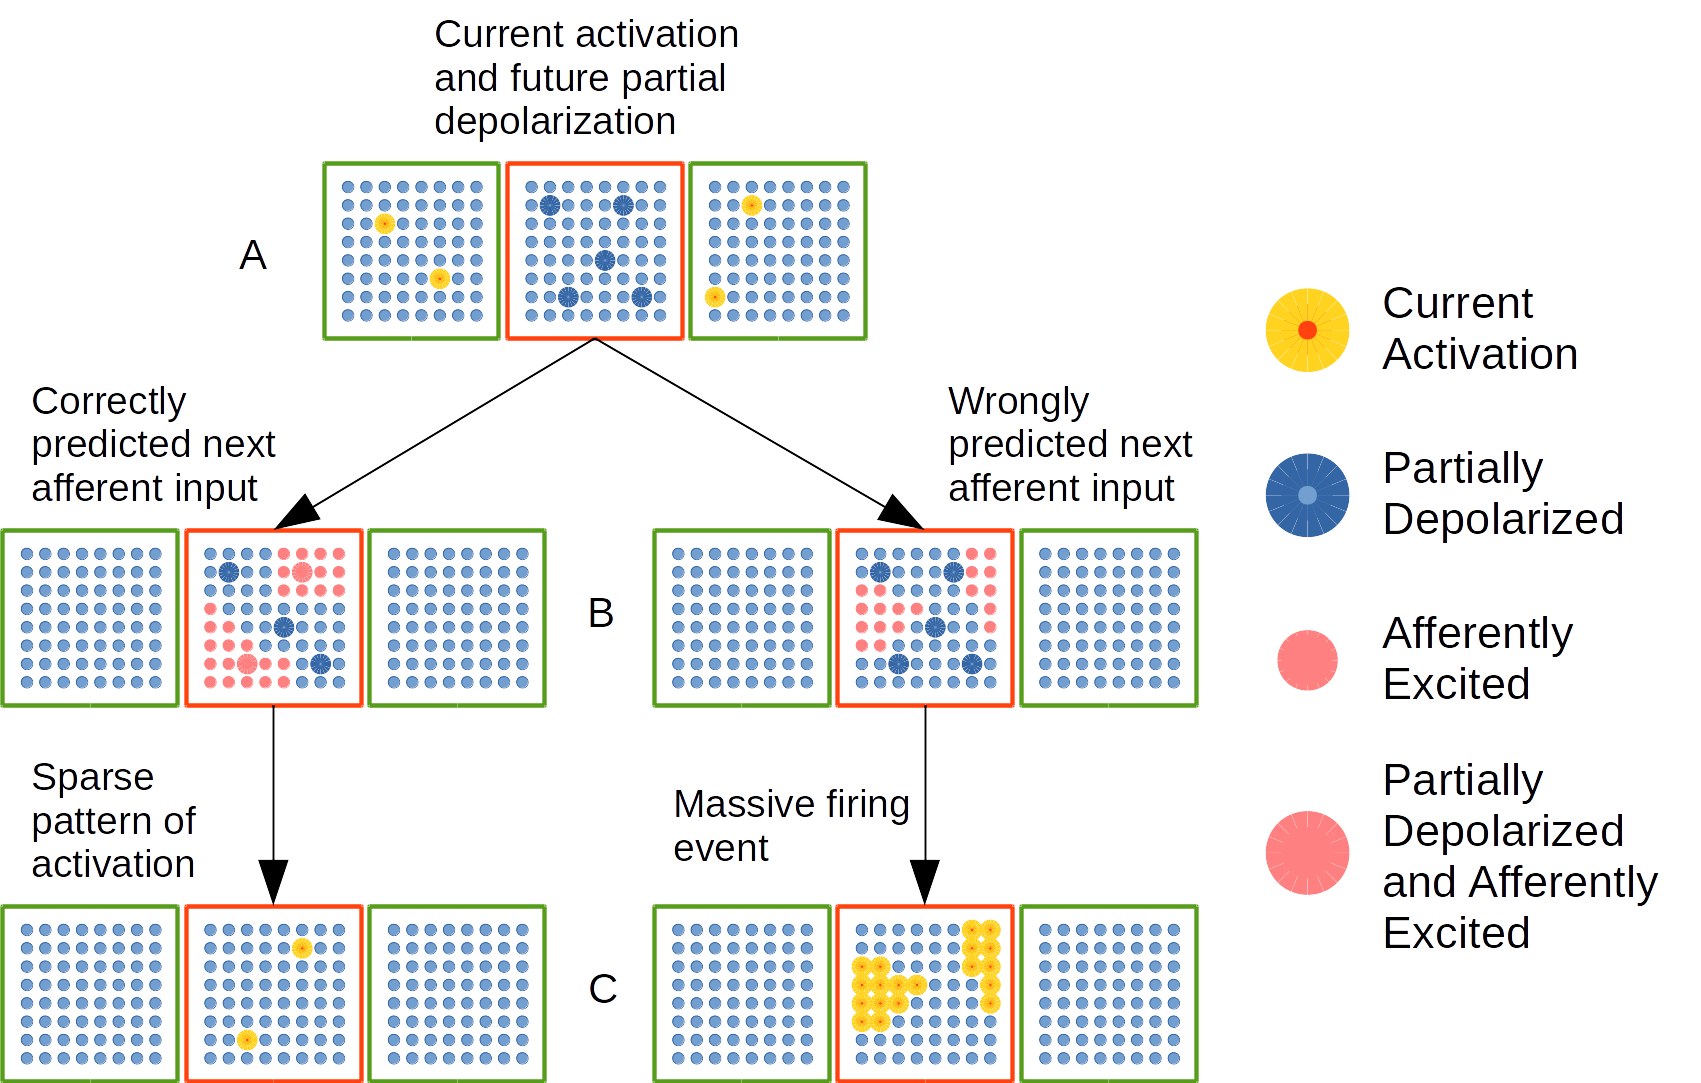
\includegraphics[width=0.8\textwidth]{Activation1.png}
    \caption{Activación celular dinámica en una \gls{cc} en la \gls{el}.
    Una columna cortical roja se vincula a dos columnas corticales verdes por medio de dendritas distales.
    \textbf{(A)} Activación celular en \gls{cc_pl} verdes--células resaltadas en amarillo--pone a las unidades neuronales
    en la \gls{cc} roja en un estado de depolarización parcial--estado predictivo resaltado en azul.
    \textbf{(B)} Cúmulos de células neuronales activadas por entradas aferentes.
    Izquierda: Una cantidad considerable de células parcialmente depolarizadas están dentro de los cúmulos celulares aferentemente excitados.
    Derecha: No hay una cantidad suficiente de células parcialmente depolarizadas dentro de los cúmulos celulares aferentemente excitados.
    \textbf{(C)} \gls{cc} con unidades celulares activas resaltada en amarillo.
    Izquierda: Patrón disperso de activación celular.
    Derecha: Patrón masivo de activación.
    Imagen adaptada de https://doi.org/10.1371/journal.pone.0217966 bajo licencia CC-BY.}
    \label{fig:Activation1}
\end{figure}

En la Fig. \ref{fig:Activation1} A, la activación actual de unidades neuronales en \gls{cc_pl} verdes más las sinapsis dendríticas distales establecidas después del aprendizaje, depolarizan parcialmente unidades neuronales específicas en la \gls{cc} roja.
Tales unidades parcialmente depolarizadas se establecen como unidades con alta probabilidad de disparar para el arribo del evento lexical siguiente.
En la Fig. \ref{fig:Activation1} B, restricciones semánticas aferentes desde el constituyente oracional siguiente excitan cúmulos de unidades neuronales específicos en la \gls{cc} roja.
A la izquierda, tales cúmulos de unidades excitadas aferentemente contienen suficientes unidades parcialmente depolarizadas las cuales se activaran antes que sus contendientes en los cúmulos excitados y--como consecuencia de ello--podrán inhibir la activación de dichas unidades contendientes como se muestra en la Fig. \ref{fig:Activation1} C a la izquierda.
De esta forma, el evento lexical actual es predicho correctamente por la red.
En la parte derecha de la Fig. \ref{fig:Activation1} B, los cúmulos excitados aferentemente no contienen un cantidad suficiente de unidades depolarizadas parcialmente, lo cual implica que la gran mayoría de las unidades en los cúmulos están en la misma condiciones para disparar.
Esta circunstancia determina que todas las unidades en los cúmulos aferentemente excitados dispararán produciendo un \gls{mfe} como el mostrado a la derecha en la Fig. \ref{fig:Activation1} C. 
Tal evento indica que la red no está prediciendo correctamente la secuencia de constituyentes lexicales en la oración.
}{
\subsection{Cortical Activation in the \gls{el}}

The dynamics of cellular activation in the \gls{el} is depicted in Fig. \ref{fig:Activation1}.
Repeated correlation among \gls{ds} afferent, sequential lateral and coarse-grained word category apical constraints determines the strength of distal dendritic synapses in such a way that certain events will be more predictable than others. As long as the sequence of sentence constituents keeps a certain level of predictability with respect to the training material, activation patterns in the \gls{el} will return enough sparsity, and a phenomenon of repeated \glspl{sdr} will be sustained throughout time. When unlikely events--with respect to training material--arise, sparsity cannot be sustained by the network and a phenomenon called \gls{mfe} will emerge as a consequence of the inability of the network to correctly predict such events. As a result of the ignorance of the network to correctly predict an event, it activates all likely hypotheses given the semantic constraints. In this way, the \gls{el} loses the bias established by syntactic constraints, opening more hypotheses in order to receive subsequent lexical events in a better condition.

\begin{figure}[ht!]
    \centering
    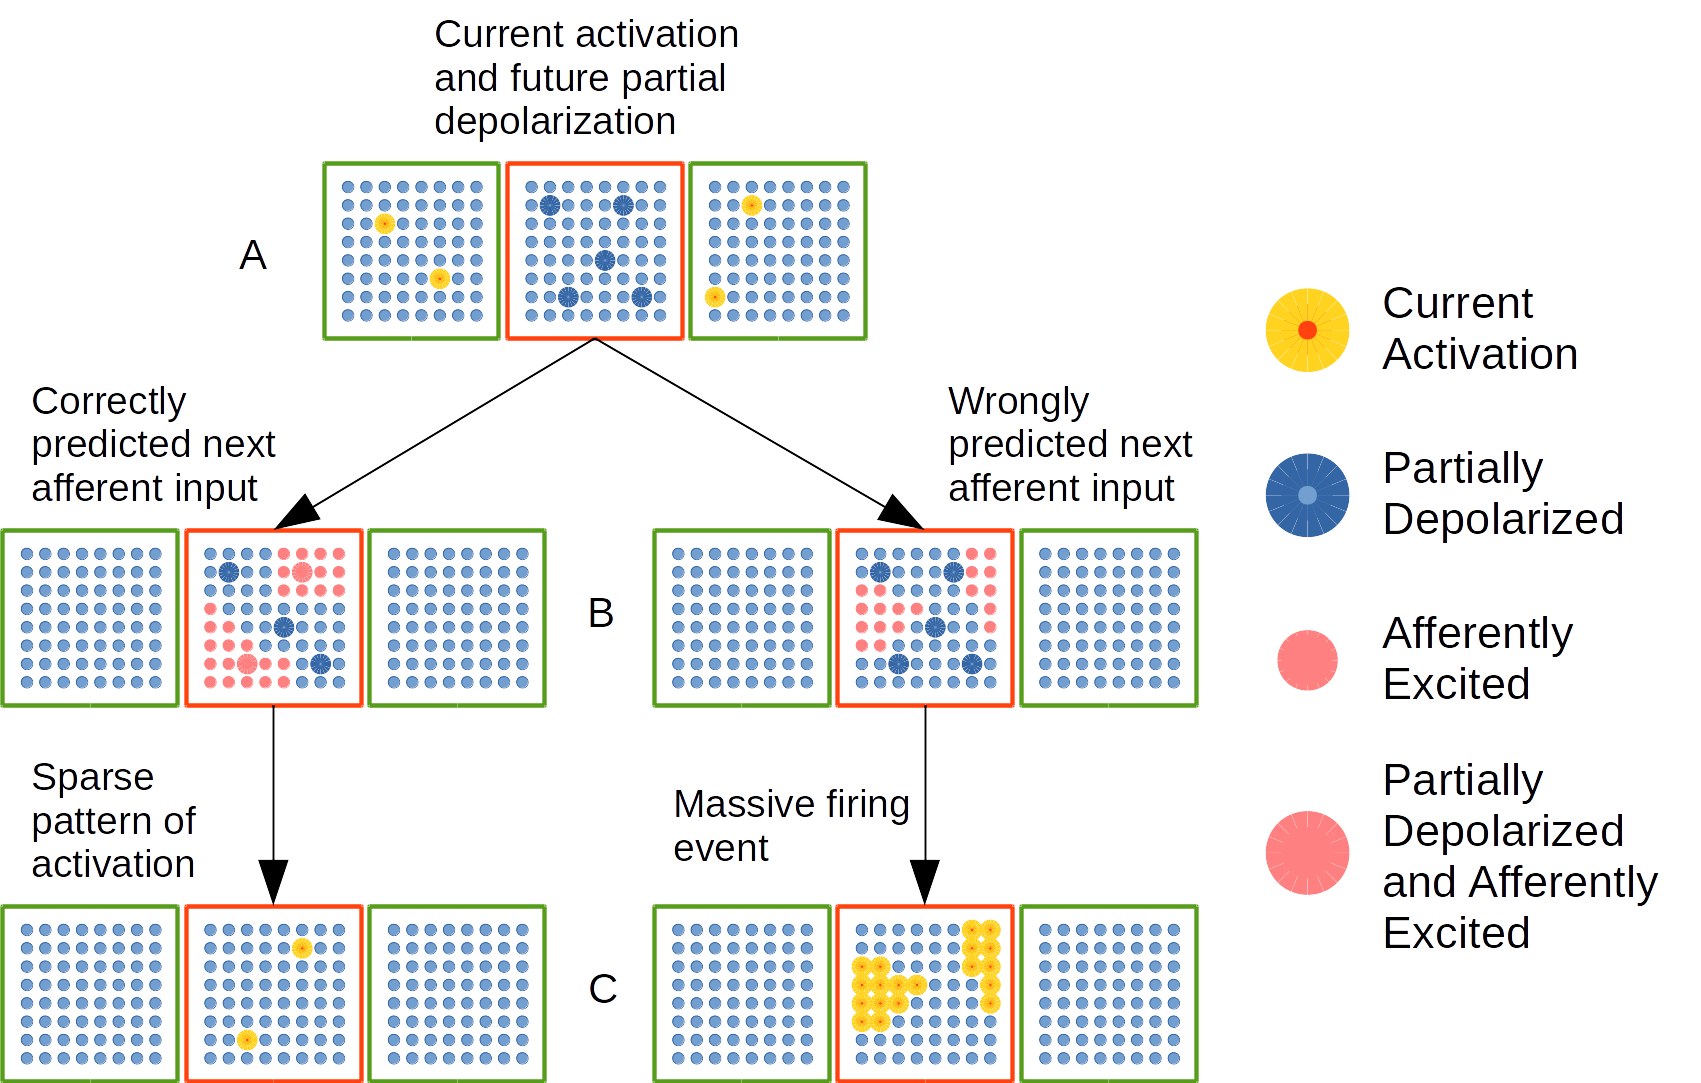
\includegraphics[width=0.8\textwidth]{Activation1.png}
    \caption{Dynamic cellular activation in a \gls{cc} in the \gls{el}.
    A red cortical column is linked with two green cortical columns by means of distal dendrites.
    \textbf{(A)} Cellular activation in green \glspl{cc}--highlighted yellow cells--puts neural units
    in red \gls{cc} in a partially depolarized--predictive state highlighted in blue.
    \textbf{(B)} Cluster of neural cells activated by afferent inputs.
    Left: A substantial amount of partially depolarized cells are in the afferently excited cellular clusters.
    Right: There is no substantial amount of partially depolarized cells inside afferently excited cellular clusters.
    \textbf{(C)} \gls{cc} with active cellular units highlighted in yellow.
    Left: Sparse pattern of cellular activation.
    Right: Massive pattern of activation.
    Adapted from https://doi.org/10.1371/journal.pone.0217966 under CC-BY license.}
    \label{fig:Activation1}
\end{figure}

In Fig. \ref{fig:Activation1} A, current activation of neural units in green \glspl{cc} plus distal dendritic synapses established after learning, partially depolarize specific neural units in the red \gls{cc}. Such partially depolarized units are set as predictable firing units for the arrival of the next lexical event. In Fig. \ref{fig:Activation1} B, afferent semantic constraints from the next sentence constituent excite specific clusters of neural units in the red \gls{cc}. On the left, such clusters of afferently excited units contain enough partially depolarized units which will activate before rival units in the excited clusters and--as a consequence of that--will be able to inhibit rival units activation as shown in Fig. \ref{fig:Activation1} C on the left. In such way, the current lexical event is correctly predicted by the network. On the right side of Fig. \ref{fig:Activation1} B, the afferently exited clusters do not contain enough partially depolarized units, which implies that the great majority of the units in the clusters are in very similar conditions to fire. This circumstance determines that all the units in the afferently excited clusters will fire producing a \gls{mfe} as shown in Fig. \ref{fig:Activation1} C on the right. Such event indicates that the network is not correctly predicting the sequence of lexical constituents in the sentence.
}
























\iftoggle{DEBUG}{
\subsection{Perfil Experimental}

El perfil experimental utilizado en este trabajo se muestra en la Fig. \ref{fig:Experiment1}.
Nuestra hipótesis es que la activación cortical desde la \gls{el} en respuesta a los constituyentes léxicos oracionales proveerá mejor información al algoritmo supervisado para clasificar la función gramatical de tales constituyentes que la información provista por word2vec.
Por lo tanto, utilizamos las características entregadas por word2vec y por la \gls{el} en respuesta a cada constituyente oracional para entrenar ambos clasificadores mostrados en la Fig. \ref{fig:Experiment1}.
Luego, probamos los algoritmos entrenados utilizando corpus diferentes al utilizado para el entrenamiento.


\begin{figure}[ht!]
    \centering
    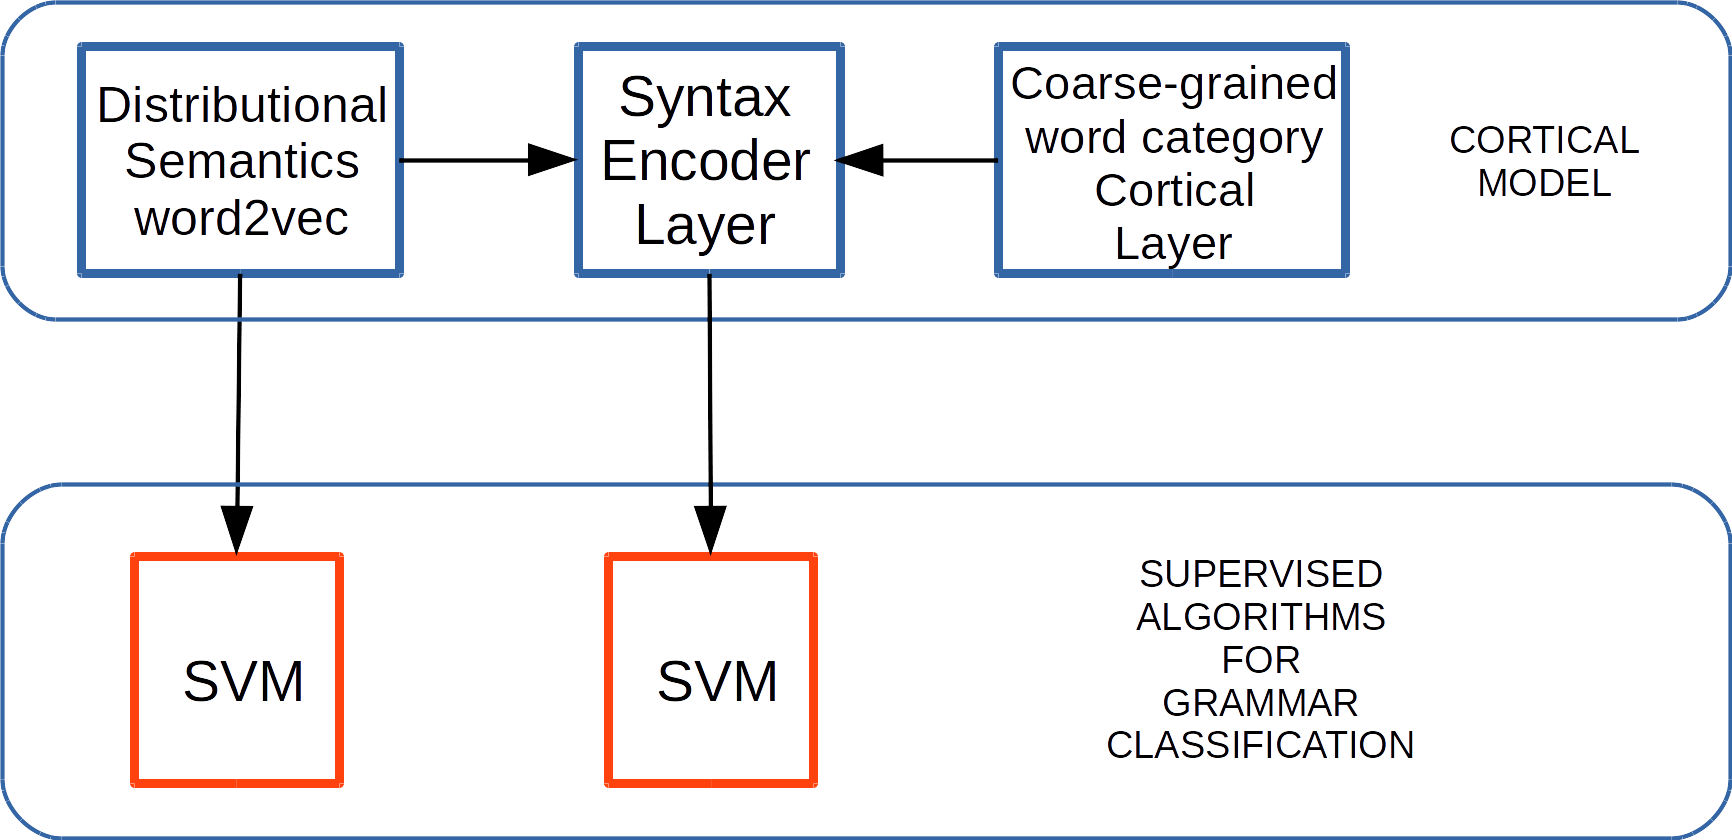
\includegraphics[width=0.8\textwidth]{Experiment1.png}
    \caption{Perfil experimental para probar el desempeño en la tarea de clasificación gramatical.
    Las restricciones en \glsfirst{ds} generadas por medio de word2vec son recibidas por las dendritas aferentes de la \gls{el}.
    Las restricciones de categorías gruesas de palabras son \gls{sdr_pl} recibidas por las dendritas apicales de la \gls{el}.
    Las tareas de clasificación de categorías gramaticales de palabras se realizan sobre ambas salidas--desde word2vec y desde la \gls{el}--por medio del algoritmo de \gls{svm}.
    Imagen adaptada de https://doi.org/10.1371/journal.pone.0217966 bajo licencia CC-BY.}
    \label{fig:Experiment1}
\end{figure}

Utilizamos supervisión por medio del método de clasificación de \gls{svm}, recibiendo las salidas de cada algoritmo.
Hicimos esto para probar las propiedades de generalización en los atributos gramaticales abstraídos por la \gls{el} en comparación con los atributos gramaticales abstraídos por word2vec (Fig. \ref{fig:Experiment1}).
Para este trabajo utilizamos un paquete de software llamado \gls{libsvm} \cite{CC01a, libsvm}.
Entrenamos y probamos los clasificadores de \gls{svm} usando validación cruzada de 5 secciones y los entrenamos para usar un kernel lineal con un parámetro $C$ el que barrimos para encontrar el mejor modelo entrenado para cada clasificador.

Implementamos una \gls{el} con 225 \gls{cc_pl} organizadas en un arreglo bidimensional de 15 por 15 \gls{cc_pl}.
Cada \gls{cc} se distribuye automáticamente utilizando posiciones individuales a lo largo de sus entradas aferentes, laterales y apicales de manera uniforme.
Cada \gls{cc} recibe información aferente por medio de campos receptivos bidimensionales de 9 por 29 componentes centrados en ubicaciones individuales sobre un espacio de 10 por 30 componentes en word2vec.
Habilitamos el uso de la propiedad \emph{envolver alrededor} (\emph{wraparound}) para hacer que cada campo receptivo se extienda a través de todo el arreglo word2vec.
También instruimos a cada columna a recibir sólo 31 entradas, lo cual es un porcentaje menor de cada campo receptivo.
Las entradas aferentes individuales para cada \gls{cc} fueron elegidas al azar durante el proceso de inicialización de la \gls{el}.

Para esta instancia del modelo utilizamos ramas dendríticas distales laterales y apicales.
Configuramos cada \gls{cc} para que tenga un campo receptivo lateral de 9 por 9 \gls{cc_pl} vecinas.
y para recibir información de 72 de las 81 \gls{cc_pl} en el campo receptivo--un 90\% del campo receptivo.
En referencia a las dendritas apicales, configuramos cada \gls{cc} para que tenga un campo receptivo apical de 11 por 11 \gls{cc_pl} foráneas y para recibir información de 108 de las 121 \gls{cc_pl} en el campo receptivo--también un 90\% del campo receptivo.

Cada \gls{cc} estuvo compuesta de un arreglo bidimensional de 15 por 15 (225) unidades neuronales y cada unidad en una columna podría conectarse potencialmente con sólo 6 unidades neuronales desde cada columna vecina vinculada.
Cada unidad neuronal en una \gls{cc} terminó teniendo 72 ramas dendríticas laterales con 6 conexiones potenciales cada una (432 sinápsis potenciales laterales distales por unidad celular) y 108 ramas dendríticas apicales con 6 conexiones potenciales cada una (648 sinápsis potenciales apicales distales por unidad celular).
Es decir, cada unidad neuronal en una \gls{cc} terminó teniendo 1080 sinápsis distales.
Tales sinápsis potenciales fueron escogidas aleatoriamente para cada célula neuronal y para cada rama dendrítica en la célula durante el procedimiento de inicialización del Encoder.
La \gls{el} consistió en 50625 unidades celulares con 1569375 sinápsis próximas y 54675000 sinápsis distales.
Es importante resaltar que las sinápsis distales representaron conexiones potenciales desde las que sólo un pequeño porcentaje tuvo un peso sináptico significativo como para ser considerada como conexión establecida.
Las sinápsis débiles son podadas periódicamente por medio de procesos homeostáticos en la red, dejando las dendritas distales con una conectividad dispersa en los campos receptivos. La dispersión en tales matrices de conectividad podría exceder el 90\%.

La \glsfirst{cl} ficticia desde la cual la \gls{el} recibe restricciones apicales--en forma de categorías gruesas de palabras en \gls{sdr_pl}--tuvo la misma configuración columnar y celular que la \gls{el}.

El procedimiento de entrenamiento consistió de 2 etapas y para cada etapa la \gls{el} recibió el mismo corpus dos veces.
Durante cada etapa de aprendizaje, ciertos parámetros--tales como las tasas de aprendizaje en las sinápsis próximas y distales y la interacción intracolumnar--se decrementaron exponencial y progresivamente desde un valor inicial.
Los mismos parámetros también se decrementaron para cada etapa sucesiva.
Una etapa adicional se ejecutó con los parámetros de aprendizaje fijos.

La dispersión en la activación para cada \gls{cc}--aún \gls{cc_pl} en la \gls{cl} de categorías gruesas de palabras--fue del 99\% (sólo 2 de 225 unidades neuronales podían activarse para eventos de activación normales).
Por otro lado, la excitación aferente afectaba el 10\% de las unidades dentro de los cúmulos en cada \gls{cc} (22 unidades neuronales, las cuales podrían activarse en el caso de un \gls{mfe}; Fig. \ref{fig:Activation1}).

Para entrenar el modelo utilizamos un corpus desde el dataset WikiSplit de Google  \cite{BothaEtAl2018}.
Este dataset fue construido automáticamente desde las revisión histórica de Wikipedia (disponible públicamente).
El dataset completo incluye un millón de oraciones en Inglés, cada una dividida en dos oraciones que juntas preservan el significado de la original, extraído desde Wikipedia edits.
Para entrenar el modelo utilizamos un corpus llamado \texttt{test} desde el dataset.
El corpus tiene 14980 oraciones. Limpiamos el corpus borrando la puntuación para obtener un archivo en el cual cada oración es una secuencia de palabras individuales en una línea.

Etiquetamos cada palabra en el corpus con su función gramatical en el contexto oracional.
Para tal fin utilizamos el analizador de lenguaje natural Enju para Inglés (Enju 2.4.4 Copyright (c) 2005-2010, Tsujii Laboratory, The University of Tokyo).
Este analizador tiene \gls{hpsg} probabilística de amplia cobertura \cite{Yusuke:2002:MEE:1289189.1289214, noauthor_2_nodate, Miyao2004CorpusOrientedGD, Miyao:2005:PDM:1219840.1219851, Ninomiya:2006:ELM:1610075.1610100, Ninomiya:2007:LMN:1621410.1621418, Miyao:2008:FFM:1350986.1350988}, así como un algoritmo de análisis eficiente \cite{tsuruoka:2004b, Ninomiya:2005:EBT:1654494.1654505, bc22fe91f8a743269f26f92abfd79790, Matsuzaki:2007:EHP:1625275.1625546}.

Enju puede efectivamente analizar estructuras sintácticas/semánticas de oraciones en Inglés y proveer al ususario con estructuras de frases y estructuras de predicado-argumento.
Esas salidas serían especialmente útiles para aplicaciones de \gls{nlp} de alto nivel, incluyendo extracción de información, sumarización automática, responder preguntas y traducción por máquinas, donde el \emph{significado} de una oración juega un rol central \cite{noauthor_english_2019}.

Analizamos gramaticalmente el corpus completo por medio de Enju en su formato stand-off.
En dicho formato cada etiqueta se representa con la posición de la oración de entrada original, cada línea representa una etiqueta.
El nombre de la etiqueta (e.g. \texttt{cons} y \texttt{tok}) se coloca primero, y el resto representa los atributos.
Un constituyente se etiqueta por \texttt{cons} mientras que cada palabra es etiquetada por \texttt{tok}.
El atributo \texttt{cat} representa el símbolo de la frase del constituyente. El atributo \texttt{pos} representa las \emph{partes del discurso} o \emph{part-of-speech} y--dentro de \texttt{tok}--el atributo \texttt{cat} representa la misma información que en \texttt{cons}.

Para etiquetar la función gramatical de las palabras en cada oración utilizamos parte de la información provista por Enju.
Específicamente usamos las etiquetas \texttt{tok} de las cuales extrajimos los atributos \texttt{cat} y \texttt{pos}.
La conjunción de esos dos atributos formó la función gramatical con la cual etiquetamos cada palabra en el contexto oracional para todo el corpus.
De esta forma terminamos teniendo 113 categorías gramaticales diferentes.

Una vez ya con todas las palabras del corpus etiquetadas, sincronizamos las \gls{sdr_pl} apicales en la etapa de entrenamiento de tal manera de que los sustantivos, adjetivos y adverbios etuvieran correlacionados con la \gls{sdr} correspondiente a las \emph{palabras de contenido}. Los artículos, auxiliares, demostrativos, cuantificadores, preposiciones, pronombres, conjunciones, etc, se correlacionaron con la \gls{sdr} correspondiente a las \emph{palabras de función}, y el resto de las palabras etiquetadas se correlacionó con la \gls{sdr} correspondiente a los \emph{verbos}.

Primero entrenamos el modelo y luego lo corrimos en modo de inferencia.
En tal modo la \gls{el} procesó la información con sus propiedades de aprendizaje deshabilitadas.
De esta manera, durante la inferencia, la \gls{el} no modificó sus sinápsis y sólo retornó patrones de activación en respuesta a los estímulos que recibía.
Luego utilizamos las salidas desde word2vec y desde las \gls{el_pl} en modo de inferencia para entrenar los clasificadores de \gls{svm} usando las etiquetas gramaticales desde Enju.
}{
\subsection{Experimental Setup}

The experimental setup used in this paper is depicted in Fig. \ref{fig:Experiment1}. Our main hypothesis is that cortical activation from the \gls{el} in response to sentence lexical constituents, will provide better information to the supervised algorithm to classify the grammatical function in such constituents than the information provided by word2vec. Therefore, we used the features delivered by word2vec and by the \gls{el} in response to each sentence constituent in order to train both classifiers shown in Fig. \ref{fig:Experiment1}. Then, we tested the trained algorithms using different corpora to the one used for training.


\begin{figure}[ht!]
    \centering
    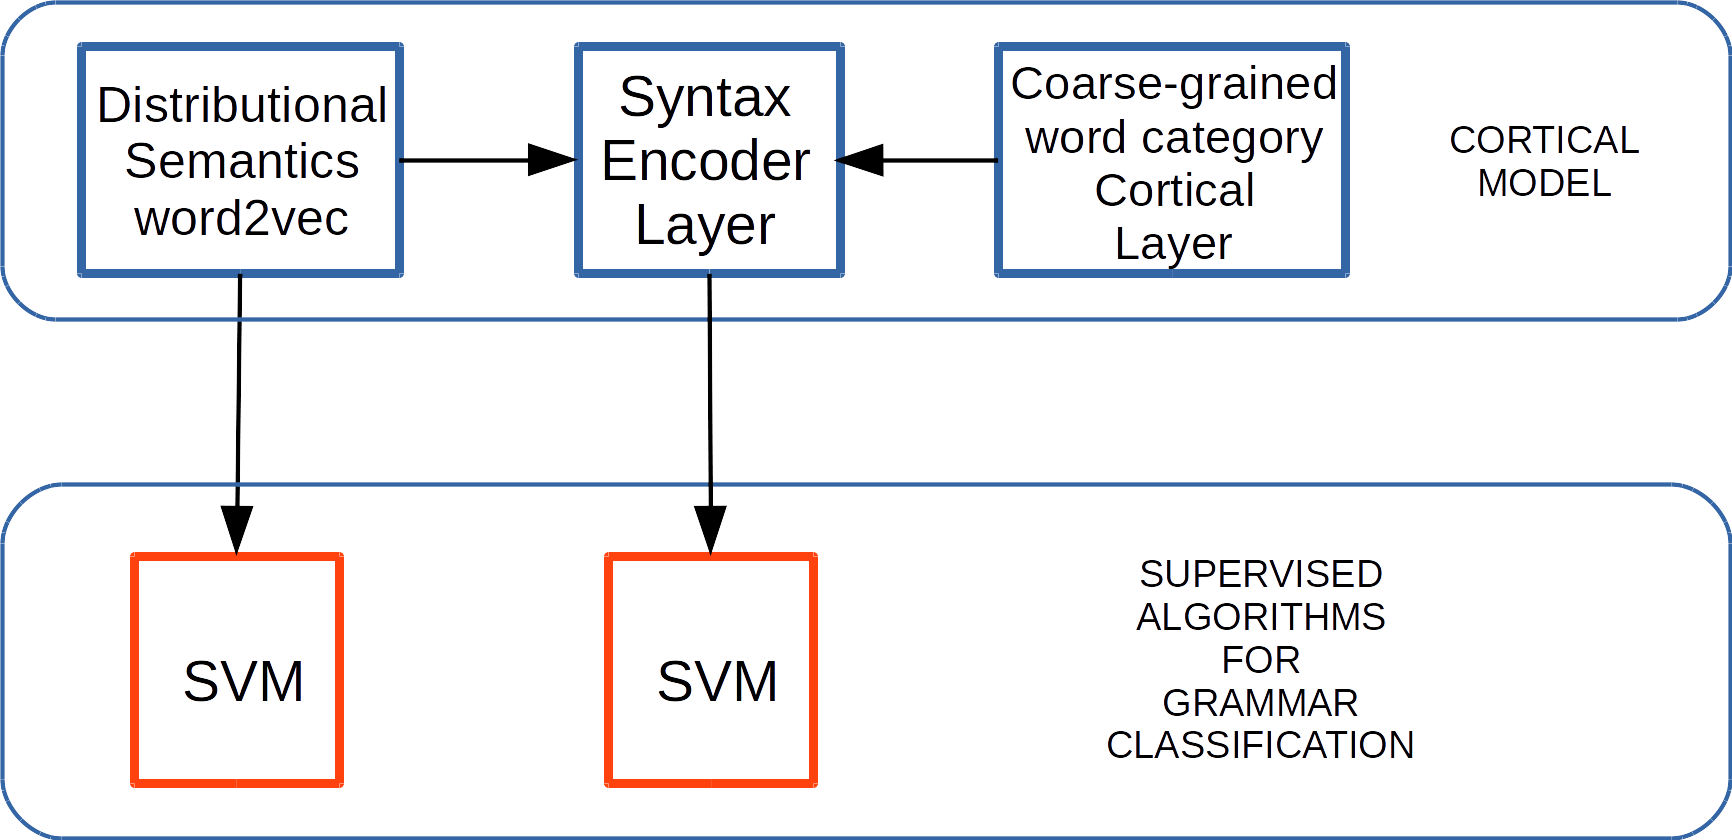
\includegraphics[width=0.8\textwidth]{Experiment1.png}
    \caption{Experimental setup to test grammar classification task performance.
    \glsfirst{ds} constraints generated by means of word2vec are received by the \gls{el} afferent dendrites.
    Coarse-grained word category constraints are \glspl{sdr} received by the \gls{el} apical dendrites.
    Grammatically-related word classification tasks are performed on both outputs--from word2vec and from the \gls{el}--by the \gls{svm} algorithm.
    Adapted from https://doi.org/10.1371/journal.pone.0217966 under CC-BY license.}
    \label{fig:Experiment1}
\end{figure}

We used supervision by means of the \gls{svm} classification method, receiving the outputs from each algorithm. We did this to test the generalization properties in the grammatical features abstracted by the \gls{el} in comparison with the grammatical features returned by word2vec (Fig. \ref{fig:Experiment1}). In the present work, we used a package called \gls{libsvm} \cite{CC01a, libsvm}. We trained and tested the \gls{svm} classifiers using 5-fold cross-validation, and configured them to use a linear kernel with one parameter $C$, which we swept to find the best trained model for each classifier.

We implemented an \gls{el} with 225 \glspl{cc} arranged in a two-dimensional array of 15 by 15 \glspl{cc}. Each \gls{cc} was automatically distributed using individual locations along its afferent, lateral and apical inputs in a uniform way. Each \gls{cc} received afferent information by means of two-dimensional afferent receptive fields of 9 by 29 components centered at individual locations over a 10 by 30 word2vec space. We enabled the wraparound property in order to make each receptive field span the entire word2vec array. We also instructed each column to receive only 31 inputs, which is a minor percentage of such receptive field. Individual afferent inputs for each \gls{cc} were chosen randomly during the \gls{el} initialization process.

For this model instance we used distal lateral and apical dendritic branches. We configured each \gls{cc} to have a lateral receptive field with 9 by 9 neighboring \glspl{cc}
and to receive information from 72 of the 81 \glspl{cc} in the receptive field--a 90\% of the receptive field. In reference to apical dendrites, we configured each \gls{cc} to have an apical receptive field of 11 by 11 foreign \glspl{cc} and to receive information from 108 of the 121 \glspl{cc} in the receptive field--also a 90\% of the receptive field.

Each \gls{cc} was composed of a two-dimensional array with 15 by 15 (225) neural units and each unit in a column could be potentially connected with only 6 neural units from each linked neighboring column. Each neural unit in a \gls{cc} ended up with 72 lateral dendritic branches with 6 potential connections each (432 distal lateral potential synapses per cellular unit) and with 108 apical dendritic branches with 6 potential connections each (648 distal apical potential synapses per cellular unit). That is, each neural unit in a \gls{cc} ended up having 1080 distal potential synapses. Such potential synapses were randomly chosen for each neural cell and for each dendritic branch in the cell during the Encoder initialization procedure. The \gls{el} consisted of 50625 cellular units with 1569375 proximal synapses and 54675000 distal synapses. It is important to highlight that distal synapses represented potential connections from which only a small percentage had a significant synaptic weight as to be considered as an established connection. Weak synapses were periodically pruned by means of homeostatic processes in the network, leaving distal dendrites with a sparse connectivity in the receptive fields. The sparseness in such connectivity matrices could exceed 90\%.

The fictitious \glsfirst{cl} from which the \gls{el} received apical constraints--in the form of coarse-grained word category \glspl{sdr}--had the same columnar and cellular configuration than the \gls{el}.

The training procedure consisted of 2 stages and for each stage the \gls{el} received the same corpus twice. During each learning stage, certain parameters--such as the learning rates in proximal and distal synapses and the lateral intra-column interaction--were exponentially and progressively decreased from an initial value. The same parameters were also decreased for each successive stage. An additional stage was executed with the learning parameters fixed.

The sparsity in the activation for each \gls{cc}--even \glspl{cc} in the coarse-grained word category \gls{cl}--was 99\% (just 2 neural units out of 225 could be active for normal activation events). On the other hand, the afferent excitation affected 10\% of the units inside the clusters in each \gls{cc} (22 neural units, which could be activated in case of a \gls{mfe}; Fig. \ref{fig:Activation1}).

In order to train the model we used a corpus from the WikiSplit dataset by Google \cite{BothaEtAl2018}. This dataset was constructed automatically from the publicly available Wikipedia revision history. The complete dataset contains one million English sentences, each split into two sentences that together preserve the original meaning, extracted from Wikipedia edits. In order to train the model we used a corpus called \texttt{test} from the dataset. The corpus has 14980 sentences. We cleaned the corpus erasing punctuation marks to get a file in which each sentence is a sequence of individual words in a line.

We tagged each word in the corpus with its grammatical function in the sentence context.
To that end we used Enju natural language parser for English (Enju 2.4.4 Copyright (c) 2005-2010, Tsujii Laboratory, The University of Tokyo).
This parser has a wide-coverage probabilistic \gls{hpsg} \cite{Yusuke:2002:MEE:1289189.1289214, noauthor_2_nodate, Miyao2004CorpusOrientedGD, Miyao:2005:PDM:1219840.1219851, Ninomiya:2006:ELM:1610075.1610100, Ninomiya:2007:LMN:1621410.1621418, Miyao:2008:FFM:1350986.1350988}, as well as an efficient parsing algorithm \cite{tsuruoka:2004b, Ninomiya:2005:EBT:1654494.1654505, bc22fe91f8a743269f26f92abfd79790, Matsuzaki:2007:EHP:1625275.1625546}.

Enju can effectively analyze syntactic/semantic structures of English sentences and provide the user with phrase structures and predicate-argument structures. Those outputs would be especially useful for high-level \gls{nlp} applications, including information extraction, automatic summarization, question answering, and machine translation, where the "meaning" of a sentence plays a central role \cite{noauthor_english_2019}. 

We analyzed the complete corpus grammatically by means of Enju in its stand-off format. In this format, the span of each tag is represented with the position in the original input sentence, each line representing a tag.  The label of a tag (e.g. "\texttt{cons}" and "\texttt{tok}") is output first, and the rest represents the attributes. A constituent is tagged by \texttt{cons} while each word is tagged by \texttt{tok}. The attribute "\texttt{cat}" represents the phrase symbol of the constituent. The attribute "\texttt{pos}" represents a part-of-speech and--inside \texttt{tok}--the attribute \texttt{cat} represents the same information as in \texttt{cons}.

To tag the grammatical function of the words in each sentence we used part of the information returned by Enju. We specifically used \texttt{tok} tags from which we extracted the attributes \texttt{cat} and \texttt{pos}. The conjunction of those two attributes formed the grammatical function with which we tagged each word in the sentence context for all the corpus. In this way, we ended up having 113 different grammatical categories. 

Once we had all the words in the corpus tagged, we synchronized apical \glspl{sdr} in the training stage in such a way that nouns, adjectives and adverbs were correlated with the \emph{content word} \gls{sdr}. Articles, auxiliaries, demonstratives, quantifiers, prepositions, pronouns, conjunctions, etc, were correlated with the \emph{function word} \gls{sdr}, and the rest of the tagged words were correlated with the \emph{verb} \gls{sdr}.

First, we trained the model, and then we ran it in inference mode. In such mode, the \gls{el} processed the information with its learning properties disabled. In this manner, during inference, the \gls{el} did not modify its synapses and just returned patterns of activation in response to the stimuli it received. We then used the outputs from word2vec and from the \glspl{el} in inference mode to train the \gls{svm} classifiers using the grammatical tags we obtained from Enju.
}






















\iftoggle{DEBUG}{
\section{Resultados}

Utilizamos las salidas desde word2vec y desde la \gls{el} in modo de inferencia para entrenar los clasificadores de \gls{svm} mostrados en la Fig. \ref{fig:Experiment1}.
Utilizamos las salidas desde tales algoritmos en respuesta a 150, 300 y 600 oraciones desde los corpus.
Los desempeños del entrenamiento con validación cruzada se muestran en el Cuadro~\ref{SVM_Training}.

\begin{table}[ht!]
\centering
\caption{Resultados del entrenamiento de la \gls{svm} con validación cruzada}
\begin{tabular}{|l|l|l|}
\hline
		& word2vec  & Capa Encoder  \\ \hline
150 Oraciones   & 84.03\%   & 89.40\%       \\ \hline
300 Oraciones   & 83.35\%   & 90.47\%       \\ \hline
600 Oraciones   & 80.96\%   & 90.79\%       \\ \hline
\end{tabular}
\label{SVM_Training}
\end{table}

Luego probamos la exactitud de la clasificación de cada algoritmo de \gls{svm}--el entrenado con 150 oraciones, el entrenado con 300 oraciones y el entrenado usando 600 oraciones--utilizando las salidas desde word2vec y desde la \gls{el} en respuesta a otras oraciones--no utilizadas para entrenar los clasificadores. 
Hicimos esto para diez conjuntos diferentes de oraciones en cada caso--esto es, 10 corpus diferentes con 150 oraciones, 10 corpus diferentes con 300 oraciones y 10 corpus diferentes con 600 oraciones.

La Fig. \ref{fig:Grammar_PLOT} muestra la exactitud promedio en clasificación devuelta por las pruebas en cada caso--esto es, corpus de 150, 300 y 600 oraciones. 

\begin{figure}[ht!]
    \centering
    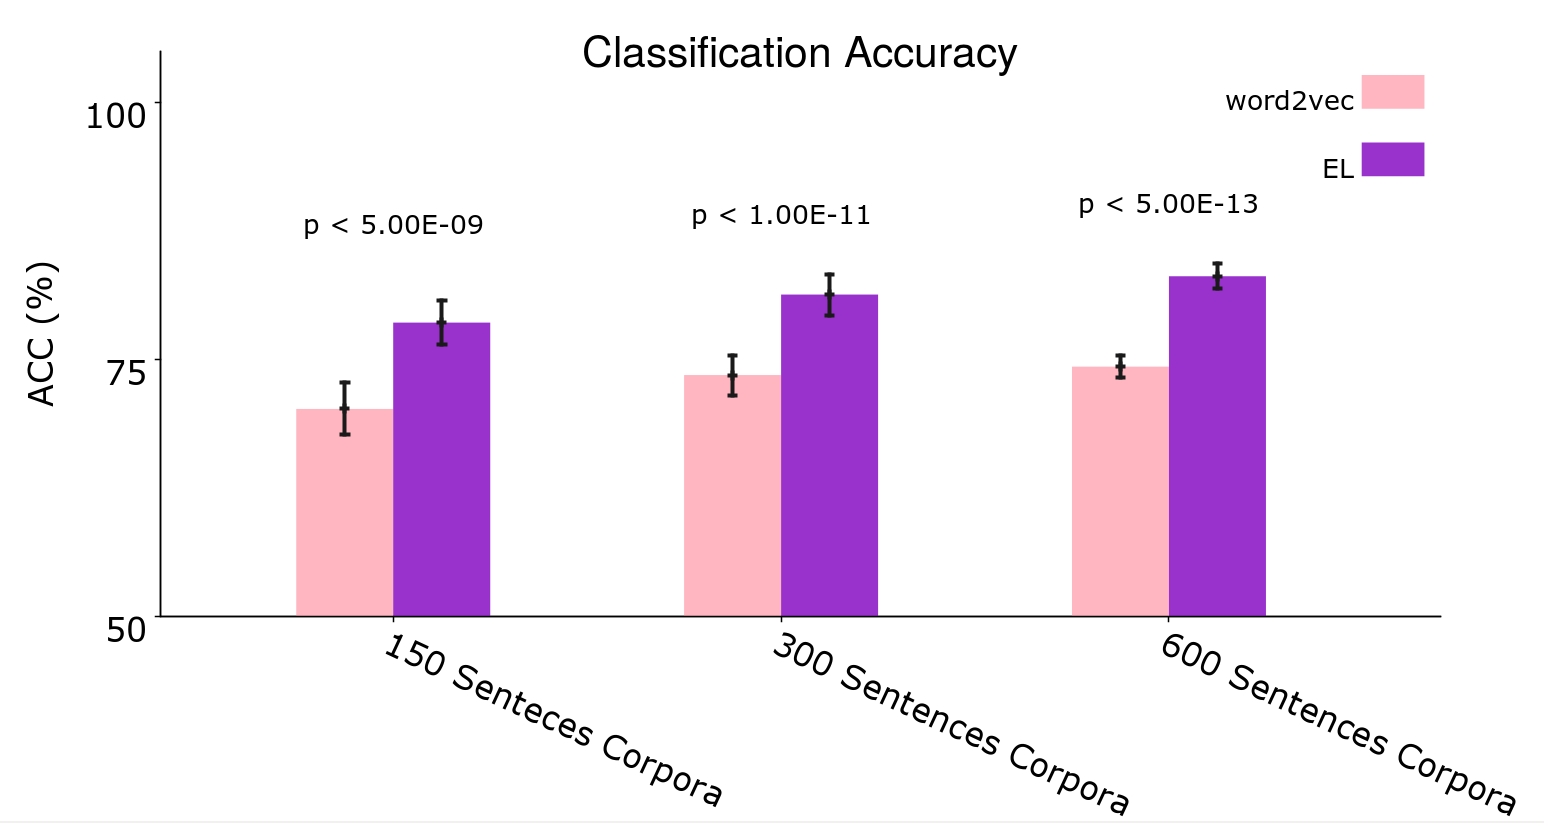
\includegraphics[width=0.8\textwidth]{Grammar_PLOT.png}
    \caption{Exactitud Promedio de Clasificación. Exactitud promedio en la clasificación de características gramaticales devueltas por word2vec vs. la \gls{el} para tres condiciones experimentales. Los valores de \emph{p} corresponden a pruebas-t de doble cola pareadas (validadas por medio de Holm-Bonferroni); cada una para 10 corpus diferentes. Las barras de error muestran Intervalos de Confianza del 95\%. Imagen Adaptada de https://doi.org/10.1371/journal.pone.0217966 bajo licencia CC-BY.}
    \label{fig:Grammar_PLOT}
\end{figure}
  
Realizamos pruebas-t pareadas de dos colas para 10 corpus diferentes desde los datos.
Dado que se realizaron 3 pruebas-t para la tarea de clasificación gramatical (es decir, para 150, 300 y 600 oraciones), utilizamos correcciones de Holm-Bonferroni con un factor de 3 para reducir la probabilidad de errores de tipo I y II en las pruebas \cite{10.1093/biomet/75.2.383}.
Como se puede observar en la Fig. \ref{fig:Grammar_PLOT} la \gls{el} se desempeña significativamente mejor que word2vec para todas las condiciones experimentales.
}{
\section{Results}

We used the outputs from word2vec and from the \gls{el} in inference mode to train the \gls{svm} classifiers shown in Fig. \ref{fig:Experiment}. We used the outputs from such algorithms in response to 150, 300 and 600 sentences from the corpus. The cross validation training performances are shown in Table~\ref{SVM_Training}.

\begin{table}[ht!]
\centering
\caption{\gls{svm} cross validation training results}
\begin{tabular}{|l|l|l|}
\hline
                & word2vec  & Encoder Layer \\ \hline
150 Sentences   & 84.03\%   & 89.40\%       \\ \hline
300 Sentences   & 83.35\%   & 90.47\%       \\ \hline
600 Sentences   & 80.96\%   & 90.79\%       \\ \hline
\end{tabular}
\label{SVM_Training}
\end{table}

We then tested the classification accuracy of each \gls{svm} algorithm--the one trained using 150 sentences, the one trained using 300 sentences and the one trained using 600 sentences--using the outputs from word2vec and the \gls{el} in response to different sentences--not used to train the classifiers. We did so for 10 different sets of sentences in each case--i.e. 10 different corpora with 150 sentences, 10 different corpora with 300 sentences and 10 different corpora with 600 sentences.

Fig. \ref{fig:Grammar_PLOT} shows the average classification accuracy returned by the tests in each case--i.e. 150, 300 and 600 sentences corpora. 

\begin{figure}[ht!]
    \centering
    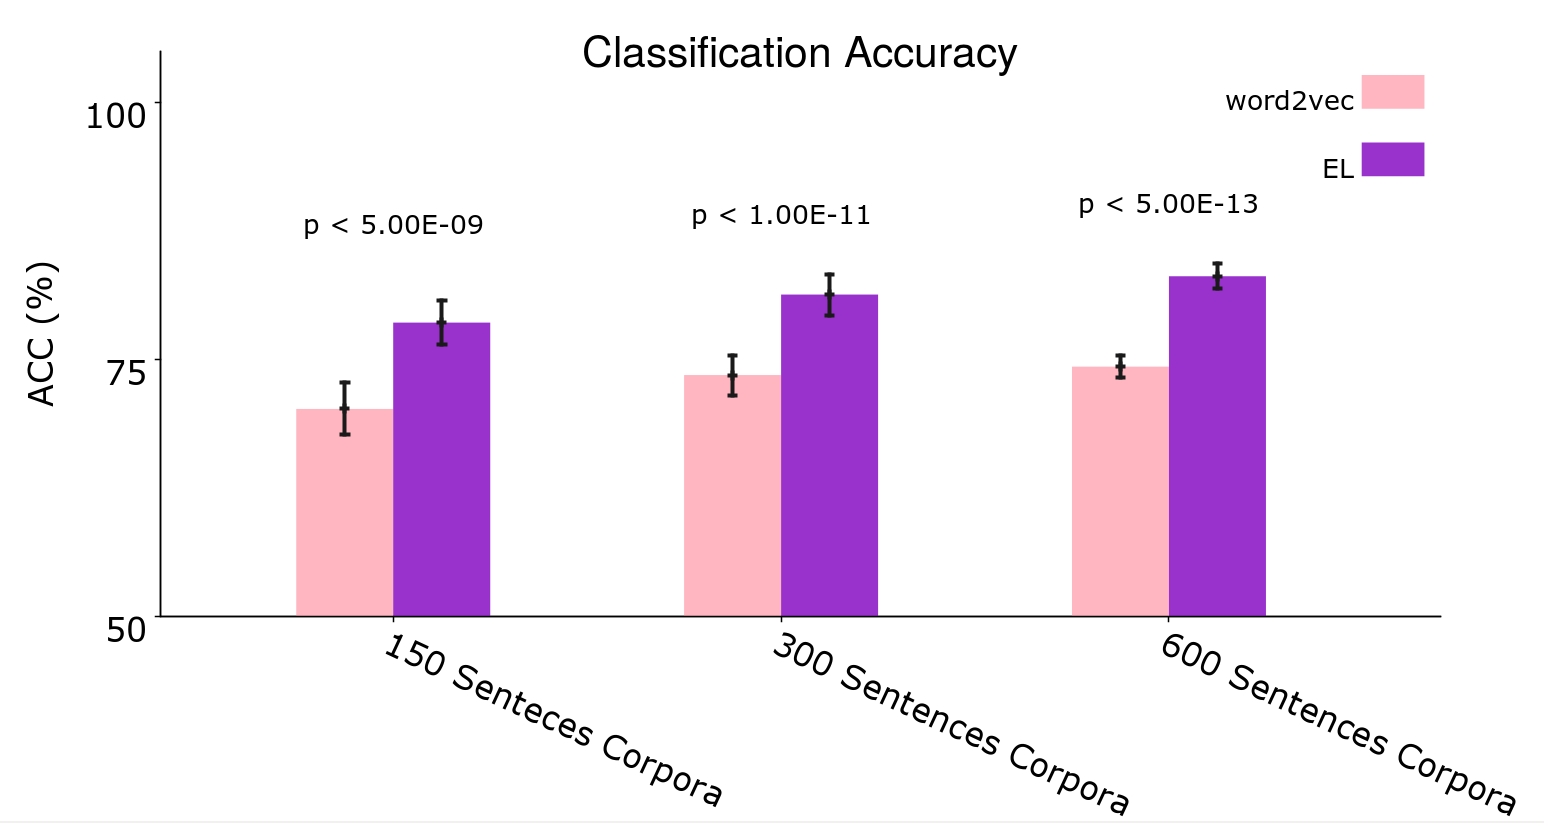
\includegraphics[width=0.8\textwidth]{Grammar_PLOT.png}
    \caption{Average Classification Accuracy. Average classification accuracy of grammatically grounded features returned by word2vec vs. features returned by the \gls{el} for three experimental conditions. The \emph{p} values correspond to two-tailed paired t-tests (Holm-Bonferroni validated); each for 10 different corpora. Error bars depict 95\% Confidence Interval values. Adapted from https://doi.org/10.1371/journal.pone.0217966 under CC-BY license.}
    \label{fig:Grammar_PLOT}
\end{figure}
  
We performed two-tailed paired t-tests for 10 different corpora from the dataset. Given that we conducted 3 t-tests for the grammar classification task (i.e. 150, 300 and 600 sentences), we performed Holm–Bonferroni corrections with a correction factor of 3 in order to reduce the probability of
type I and type II errors in the tests \cite{10.1093/biomet/75.2.383}. As can be seen in Fig. \ref{fig:Grammar_PLOT} the \gls{el} performed significantly better than word2vec in all the experimental conditions.
}


















\iftoggle{DEBUG}{
\subsection{Análisis de una Oración Individual}
\label{SentenceAnalysis}

Para ilustrar los resultados mostrados en la Fig. \ref{fig:Grammar_PLOT}, la Fig. \ref{fig:Sentence1} muestra cómo word2vec y la \gls{el} sirven a loas algoritmos de \gls{svm} para las tareas de clasificación gramatical en el contexto de la oración:

\begin{sloppypar}
\texttt{wolves feed primarily on medium to large sized ungulates though they ~~are opportunistic feeders and will generally eat any meat that is available}.
\end{sloppypar}

En la Fig. \ref{fig:Sentence1} resaltamos palabras específicas en la oración y mostramos cómo los modelos de \gls{svm} las clasifican utilizando la información producida por cada algoritmo.

\begin{figure}[ht!]
    \centering
    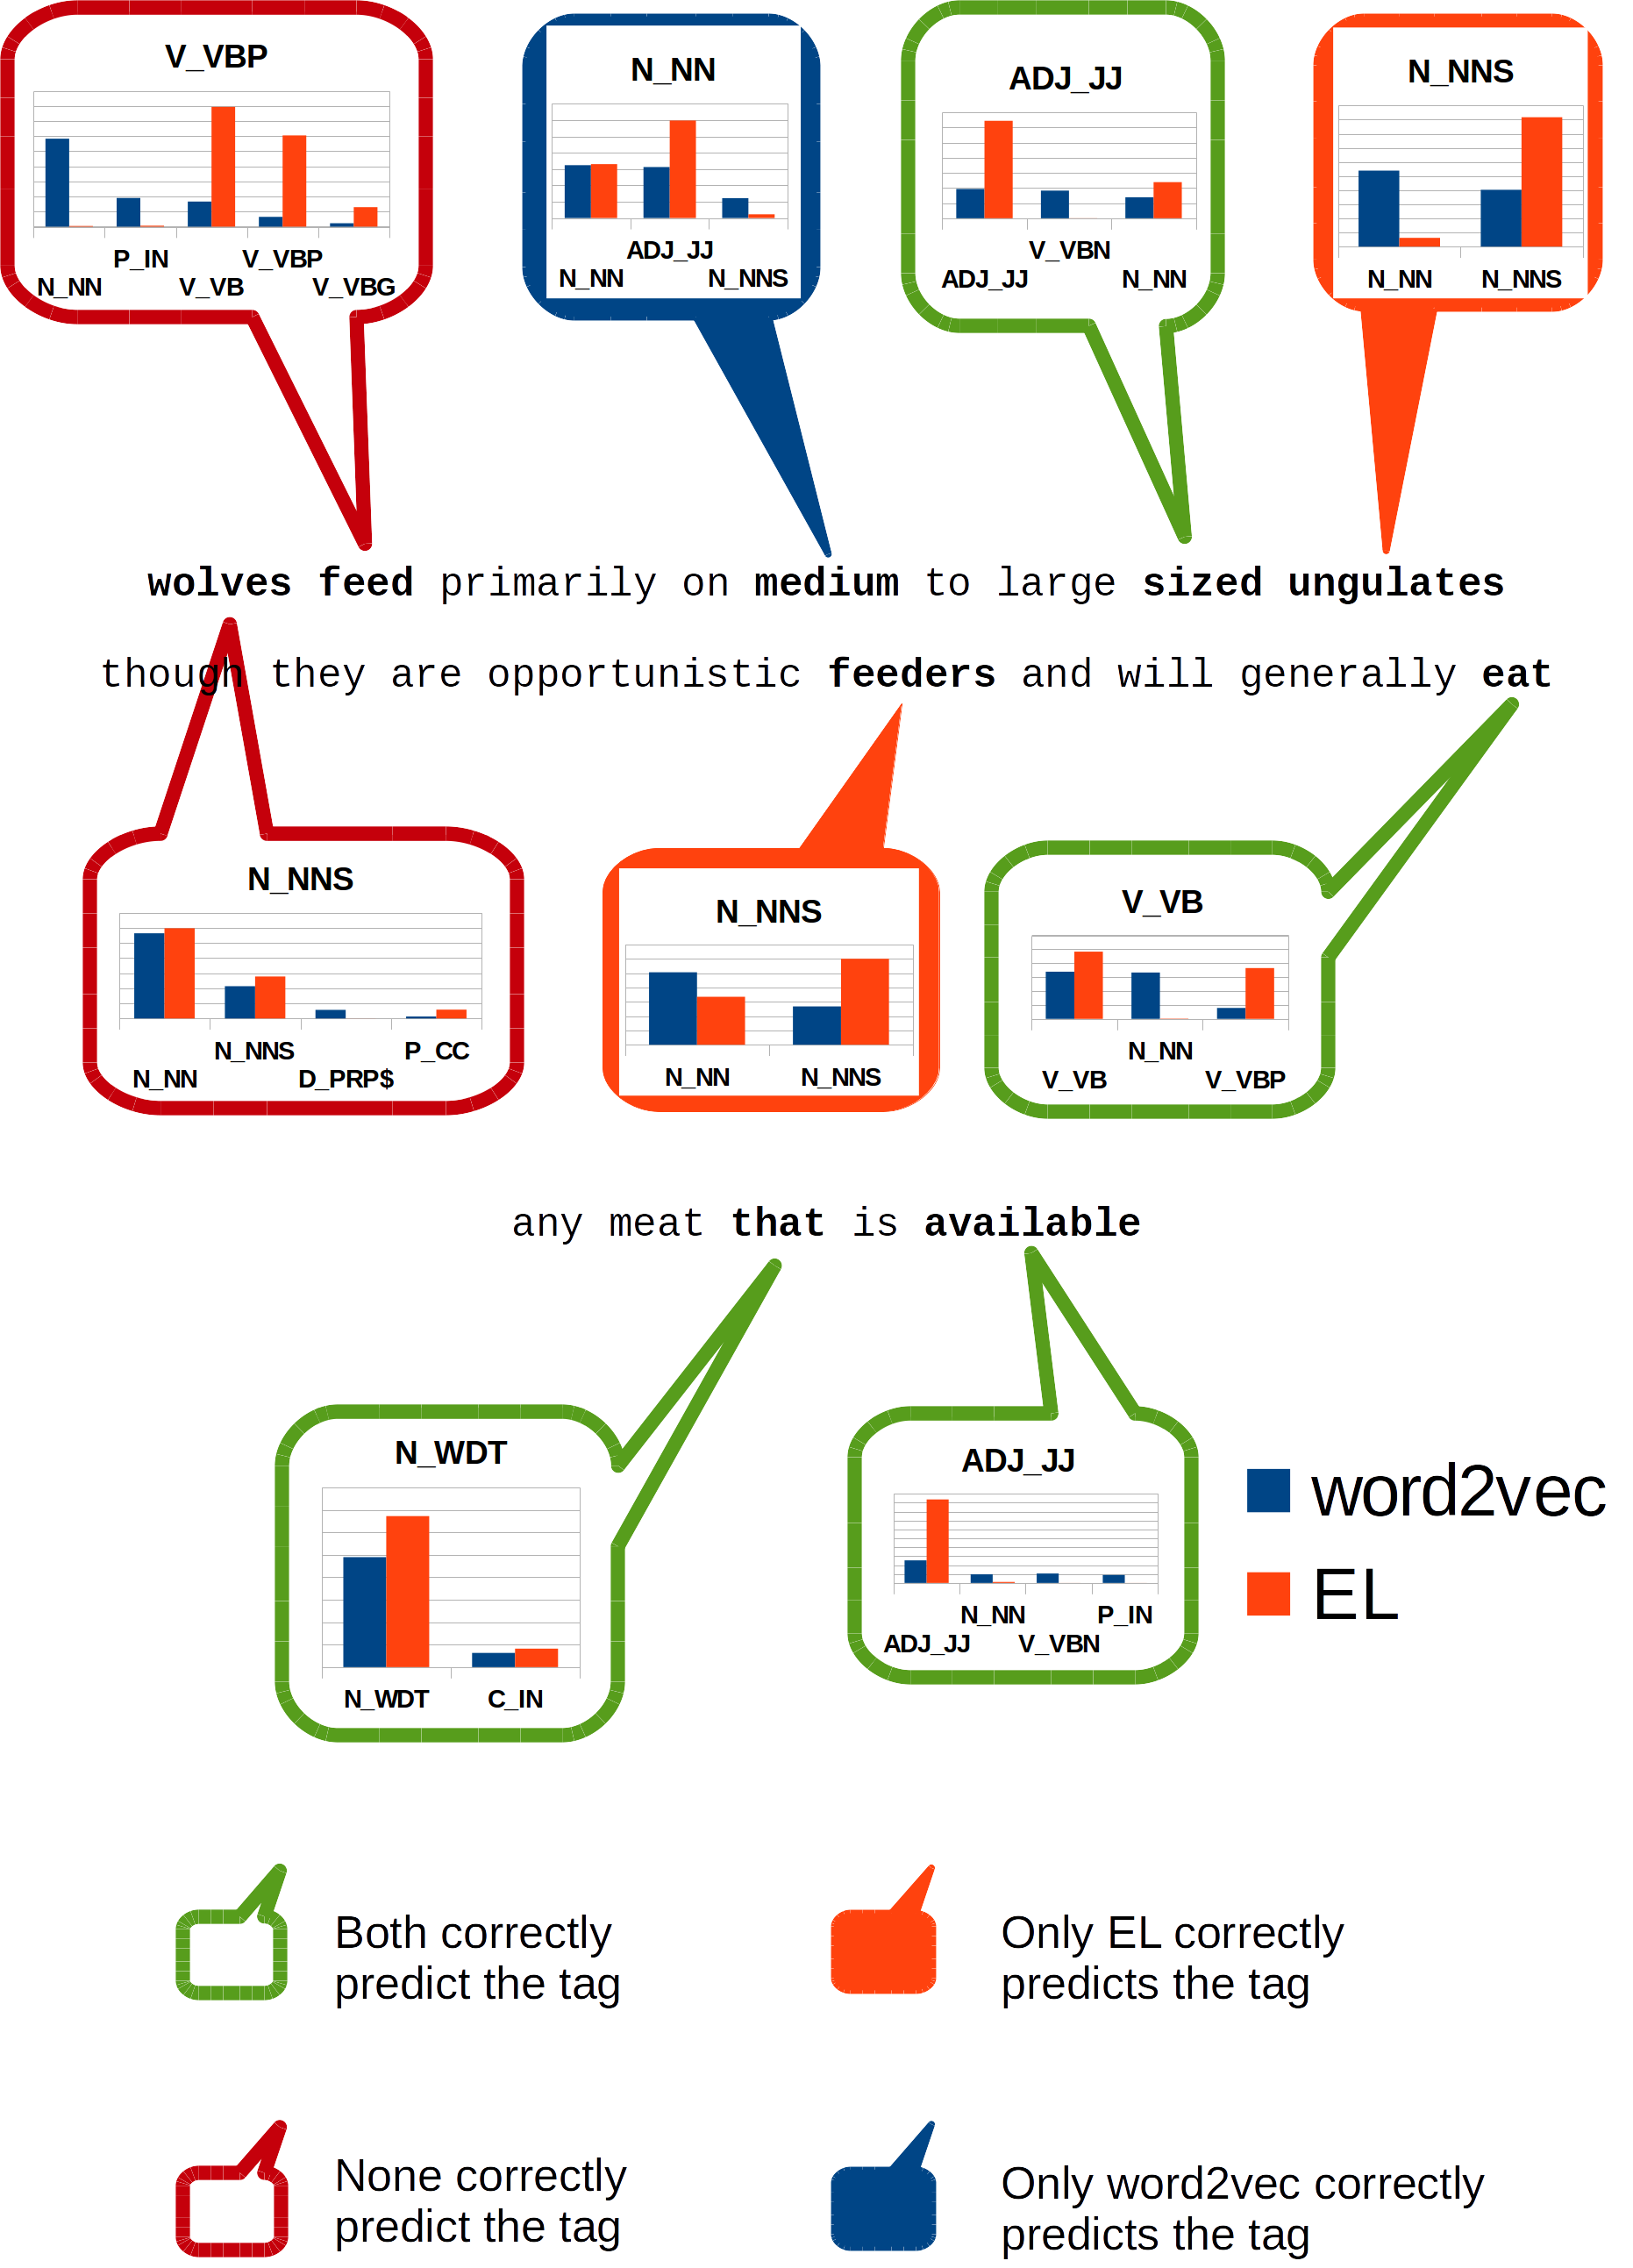
\includegraphics[width=0.8\textwidth]{Sentence1.png}
    \caption{Clasificación de los Constituyentes individuales dentro de la oración: \texttt{wolves feed primarily on medium to large sized ungulates though they are opportunistic feeders and will generally eat any meat that is available}.}
    \label{fig:Sentence1}
\end{figure}

La primera palabra (\texttt{wolves}) es clasificada de manera incorrecta por ambos algoritmos los que pierden el sentido de número en la entrada léxica la que es detectada correctamente  por nuestro clasificador modelo--Enju. La segunda palabra (\texttt{feed}) es un verbo, singular no-3ra persona en presente según el clasificador modelo. Ambos algoritmos clasifican tal constituyente también de manera incorrecta, pero esta vez existe una clara diferencia en relación a la información que cada algoritmo provee a los clasificadores. Por un lado, word2vec provee características a las que el clasificador asigna un máximo de 29\% de chance  de ser un sustantivo singular. Por otra parte, la \gls{el} provee características a las cuales el clasificador asigna 39\% de chance de ser un verbo en forma base, pero también asigna 30\% de probabilidad a la misma etiqueta asignada por el clasificador modelo--la cual es la correcta para este caso.

La palabra \texttt{medium} la que claramente actúa como un adjetivo en esta oración, es clasificada de manera errónea por el clasificador modelo como un sustantivo singular; hipótesis a la cual word2vec se pliega. Sin embargo la \gls{el} provee información a la \gls{svm} de tal manera que esta asigna casi un 60\% de probabilidad de que el constituyente es un adjetivo.

La palabra \texttt{sized} también actúa como un adjetivo en esta oración. Este constituyente es clasificado correctamente por ambos algoritmos, pero la \gls{el} provee una activación que da al algoritmo de la \gls{svm} más del 64\% de confianza en su clasificación, mientras que word2vec provee características que hacen la clasificación de la \gls{svm} considerablemente más incierta: esta asigna 19\% a la etiqueta correcta, pero también asigna 18 y 13\% a las etiquetas \emph{verbo en participio pasado} y \emph{sustantivo singular} respectivamente.

En las palabras \texttt{ungulates} y \texttt{feeders} la \gls{el} provee suficiente información al algoritmo de la \gls{svm} como para hacer que este asigne una alta probabilidad--más del 90\% para ungulates y más del 60\% para feeders--a las etiquetas correctas en ambos casos. Por otro lado, word2vec pierde el sentido de número atribuyendo la etiqueta de sustantivo singular a ambos constituyentes.

La palabra \texttt{eat} es clasificada correctamente por ambos algoritmos pero la \gls{el} asigna la probabilidad más alta a la etiqueta correcta--más que el 48\%--mientras que word2vec desperdiga chances a lo largo de un mayor rango de etiquetas incluyendo sustantivos.

Finalmente la palabra \texttt{available} fue clasificada correctamente por ambos algoritmos, pero la \gls{el} asignó con gran margen la probabilidad más alta a la etiqueta correcta--más que el 93\%--mientras que ignoraba virtualmente etiquetas alternativas como opciones viables. Por otro lado word2vec asignaba un pequeña chance del 25\% a tal etiqueta distribuyendo la probabilidad en un rango mucho más amplio de etiquetas.
}{
\subsection{Individual Sentence Analyses}
\label{SentenceAnalysis}

With the aim of illustrating the results showed by Fig. \ref{fig:Grammar_PLOT}, Fig. \ref{fig:Sentence1} shows how word2vec and the \gls{el} serve \gls{svm} algorithms for grammar classification tasks within the context of the sentence:

\begin{sloppypar}
\texttt{wolves feed primarily on medium to large sized ungulates though they ~~are opportunistic feeders and will generally eat any meat that is available}.
\end{sloppypar}

In Fig. \ref{fig:Sentence1} we highlight specific words in the sentence and show how \gls{svm} models classify them using the information produced by each algorithm.

\begin{figure}[ht!]
    \centering
    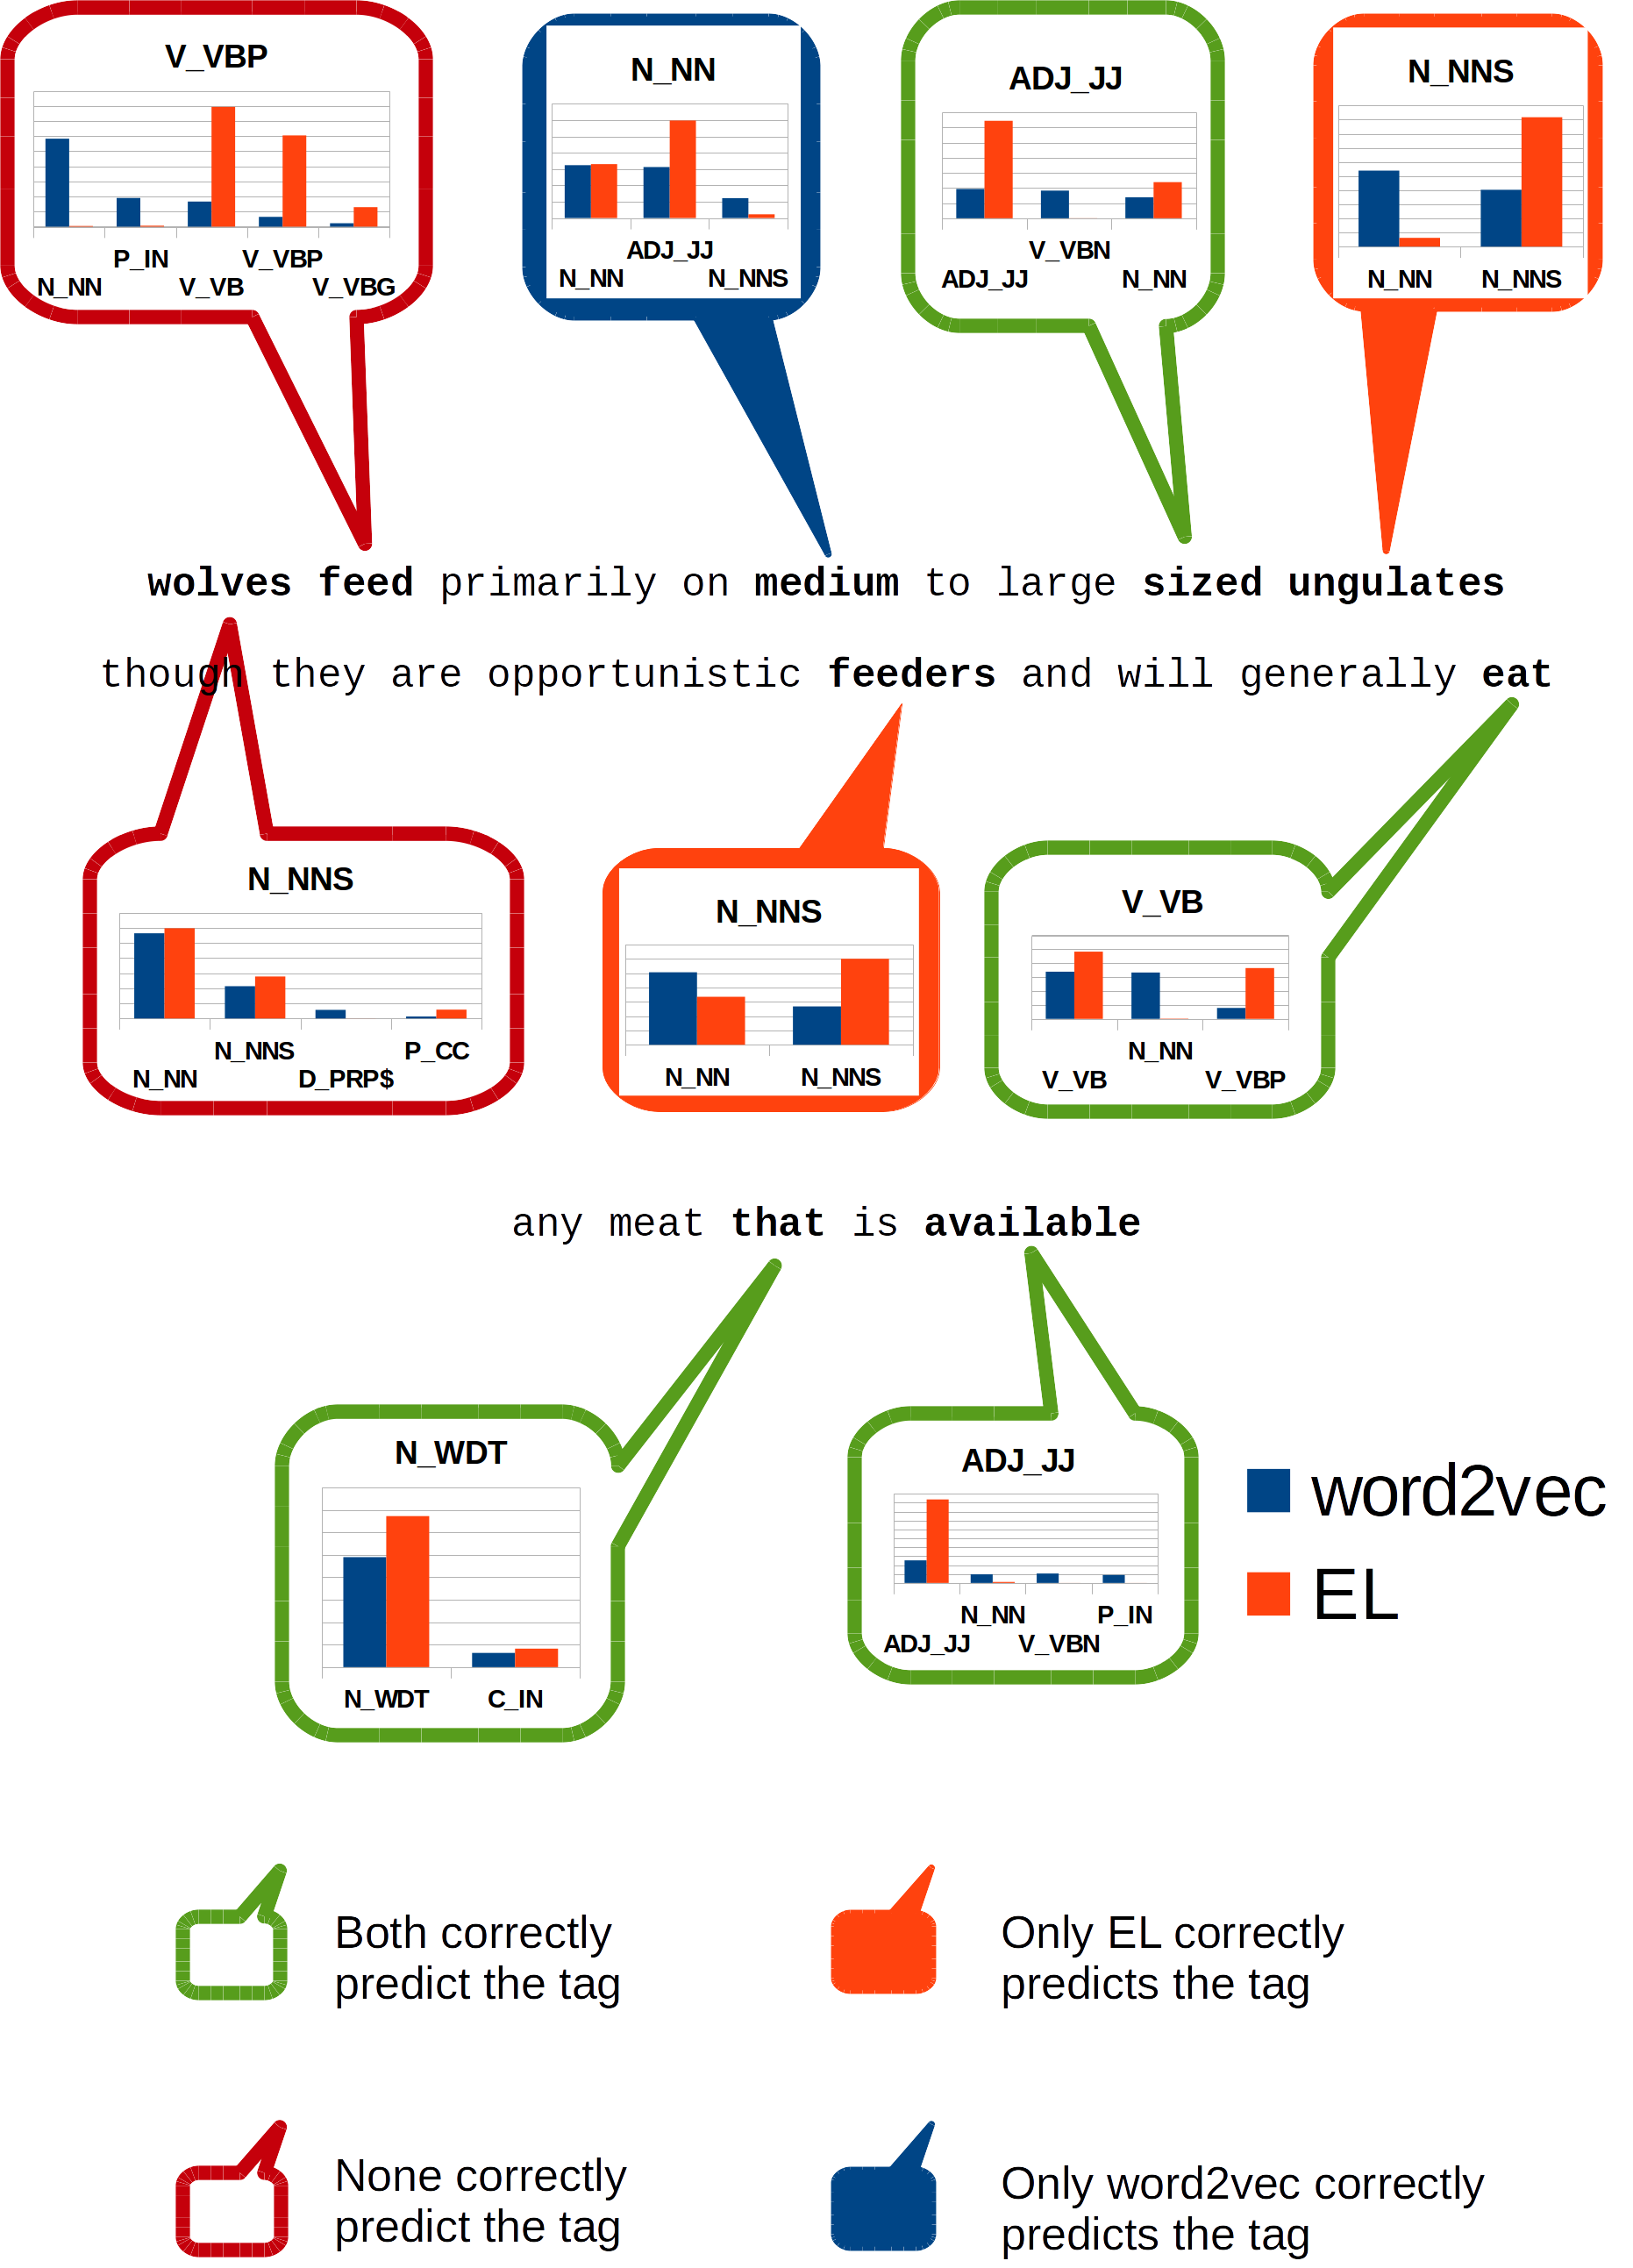
\includegraphics[width=0.8\textwidth]{Sentence1.png}
    \caption{Classification of individual constituents within the sentence: \texttt{wolves feed primarily on medium to large sized ungulates though they are opportunistic feeders and will generally eat any meat that is available}.}
    \label{fig:Sentence1}
\end{figure}

The first word (\texttt{wolves}) is incorrectly classified by both algorithms losing the number sense in the lexical entry which is correctly detected by our gold standard --Enju. The second word (\texttt{feed}) is a verb, non-3rd person singular present according to our gold standard. Both algorithms incorrectly classified such constituent too, but this time there was a clear difference regarding the information each algorithm provided the classifiers. On the one hand, word2vec provided features to which the classifier assigned a maximum of 29\% likelihood of being a singular noun. On the other hand, the \gls{el} provided features to which the classifier assigned 39\% chance of being a verb in base form, but it also assigned 30\% likelihood to the same tag assigned by the gold standard--which is the correct one for this case.

The word \texttt{medium} which clearly acts as an adjective in this sentence, is missclassified by our gold standard as a singular noun; hypothesis to which word2vec endorses. Nonetheless, the \gls{el} provides information to the \gls{svm} such that it assigns almost 60\% probability that this sentence constituent is an adjective.

The word \texttt{sized} acts as an adjective in this sentence too. This constituent is correctly classified by both algorithms, but the \gls{el} provides activation which gives the \gls{svm} algorithm more than 64\% confidence about its classification, while word2vec provides features that turns the \gls{svm} classification considerably more undetermined: it assigned 19\% to the correct tag, but in addition it also assigned 18 and 13\% to the tags "verb in past participle" and "singular noun" respectively.

In the words \texttt{ungulates} and \texttt{feeders} the \gls{el} provided enough information to the \gls{svm} algorithm as to make it assign a high probability--more than 90\% for ungulates and more than 60\% to feeders--to the correct tags in both cases. On the other hand, word2vec lost the number sense attributing a singular noun tag to both constituents.

The word \texttt{eat} is correctly classified by both algorithms but the \gls{el} assigns the highest probability to the correct tag--more than 48\%--while word2vec spreads chance out along a larger range of tags including nouns.

Finally, the word \texttt{available} was correctly classified by both algorithms, but the \gls{el} assigned by far the highest probability to the correct tag--more than 93\%--while virtually neglecting alternative tags as viable options. On the other hand, word2vec assigned a scarce 25\% chance to such tag, distributing the probability throughout a much larger range of tags.
}

















\iftoggle{DEBUG}{
\subsection{Testeando una Capa Encoder sin Conexiones Laterales}
\label{slc}

A los fines de analizar cómo contribuyen las diferentes ramas dedríticas en el modelo en relación a la tarea de clasificación, utilizamos una instancia de la \gls{el} pero esta vez removimos todas las conexiones laterales--esta instancia de la \gls{el} es llamada \gls{elslc}.
Entrenamos y probamos esta instancia usando el mismo procedimiento descripto arriba.
Los desempeños de entrenamiento con validación cruzada comparando la versión de la \gls{el} con la nueva instancia sin conexiones laterales se muestran en el Cuadro~\ref{SVM_Training1}.

\begin{table}[ht!]
\centering
\caption{Resultados del entrenamiento de \gls{svm} con validación cruzada comparando una \gls{elslc} con la \gls{el} normal}
\begin{tabular}{|l|l|l|}
\hline
		& CE SCL  & CE \\ \hline
150 Oraciones   & 88.03\%   & 89.40\%       \\ \hline
300 Oraciones   & 89.16\%   & 90.47\%       \\ \hline
600 Oraciones   & 87.07\%   & 90.79\%       \\ \hline
\end{tabular}
\label{SVM_Training1}
\end{table}


Así como hicimos anteriormente, probamos la exactitud de clasificación de cada algoritmo de \gls{svm}--el entrenado utilizando 150 oraciones, el entrenado utilizando 300 oraciones y el entrenado utilizando 600 oraciones--usando las salidas desde la \gls{elslc} y la \gls{el} en respuesta a oraciones diferentes--no utilizadas para entrenar los clasificadores.

La Fig. \ref{fig:PLOT2} muestra la exactitud de clasificación promedio comparando la \gls{el} con la \gls{elslc}.


\begin{figure}[ht!]
    \centering
    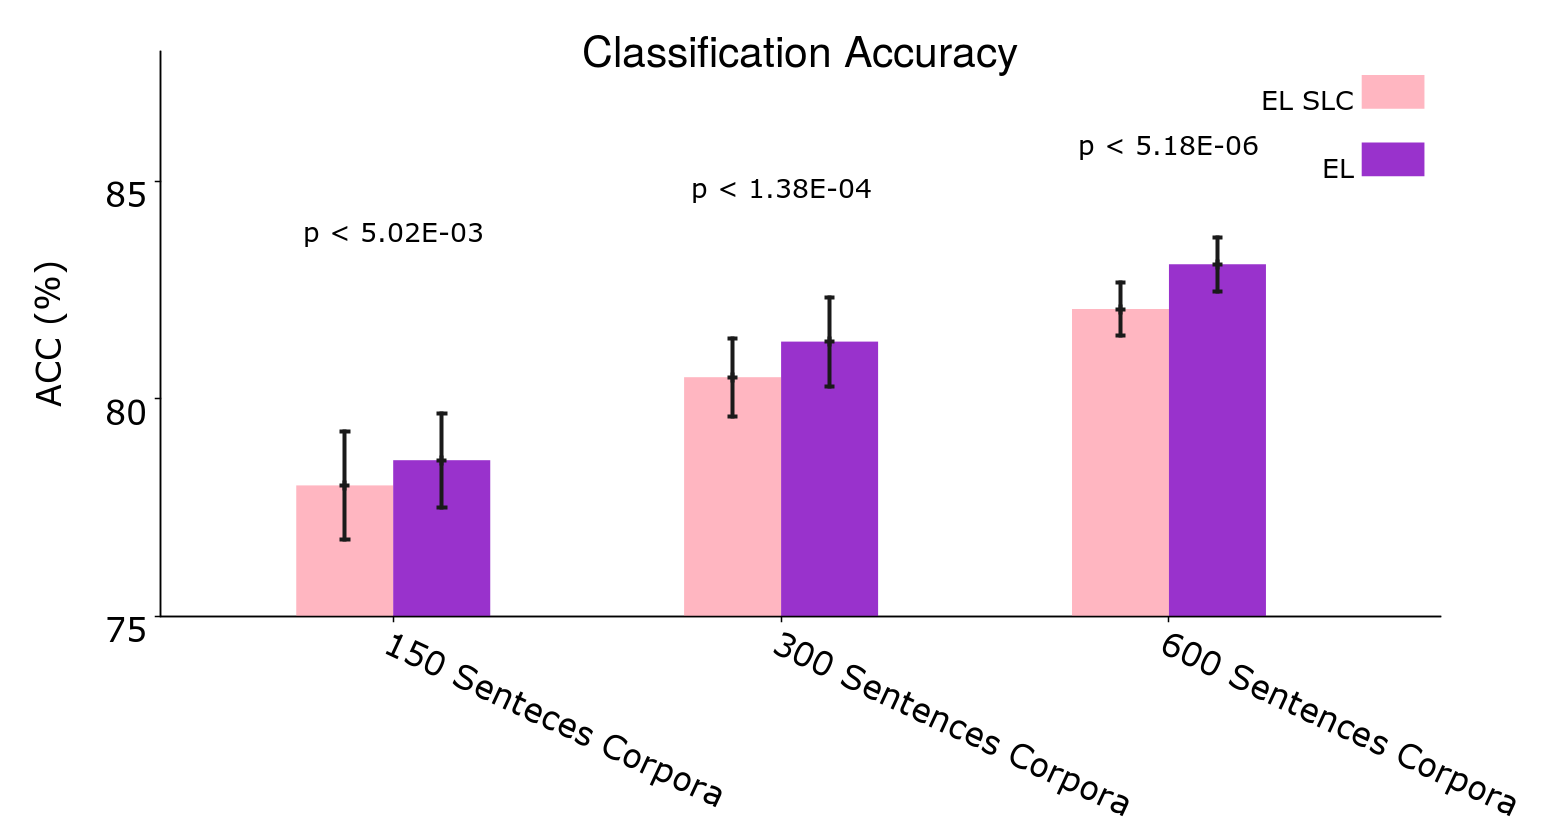
\includegraphics[width=0.8\textwidth]{PLOT2.png}
    \caption{Exactitud Promedio de Clasificación. Exactitud promedio de clasificación de características gramaticales devueltas por la \gls{elslc} vs. características devueltas por la \gls{el} para tres condiciones experimentales. Los valores de \emph{p} corresponden a pruebas t de doble cola pareadas (validadas con Holm-Bonferroni); cada una para 10 corpus diferentes. Las barras de error muestran los valores de intervalos de confianza del 95\%. Imagen adaptada de https://doi.org/10.1371/journal.pone.0217966 bajo licencia CC-BY.}
    \label{fig:PLOT2}
\end{figure}

Una vez más realizamos pruebas t de doble cola pareadas para 10 corpus diferentes desde los datos y aplicamos correcciones de Holm-Bonferroni con un factor de 3.
Como muestra la Fig. \ref{fig:PLOT2}, la \gls{el} normal se desempeña ligeramente mejor que la \gls{elslc}.
Esta diferencia global en el desempeño es estadísticamente significativa para todas las condiciones experimentales de acuerdo a las pruebas t.
Un análisis estadístico desagregado mostrando cómo las dendritas distales laterales contribuyen en la clasificación de categorías sintácticas diferentes se desarrolla en la sección \ref{Segregated}.
}{
\subsection{Testing an EL with Stripped Lateral Connections}
\label{slc}

In order to analyze the contributions provided by the two different distal dendritic trees in the model in regards to the classification task, we tested an instance of the \gls{el} but this time we stripped all its lateral connections--we call this \gls{el} instance as \gls{elslc}. We trained and tested this instance using the same procedure depicted above.
The cross validation training performances comparing the normal version of the \gls{el} with the new instance without lateral connections are shown in Table~\ref{SVM_Training1}.

\begin{table}[ht!]
\centering
\caption{\gls{svm} cross validation training results on the comparison between an \gls{elslc} and a normal \gls{el}}
\begin{tabular}{|l|l|l|}
\hline
                & EL SLC  & EL \\ \hline
150 Sentences   & 88.03\%   & 89.40\%       \\ \hline
300 Sentences   & 89.16\%   & 90.47\%       \\ \hline
600 Sentences   & 87.07\%   & 90.79\%       \\ \hline
\end{tabular}
\label{SVM_Training1}
\end{table}


As before, we tested the classification accuracy of each \gls{svm} algorithm--the one trained using 150 sentences, the one trained using 300 sentences and the one trained using 600 sentences--using the outputs from the \gls{elslc} and the \gls{el} in response to different sentences--not used to train the classifiers.

Fig. \ref{fig:PLOT1} shows the average classification accuracy comparing the normal \gls{el} with the \gls{elslc}.


\begin{figure}[ht!]
    \centering
    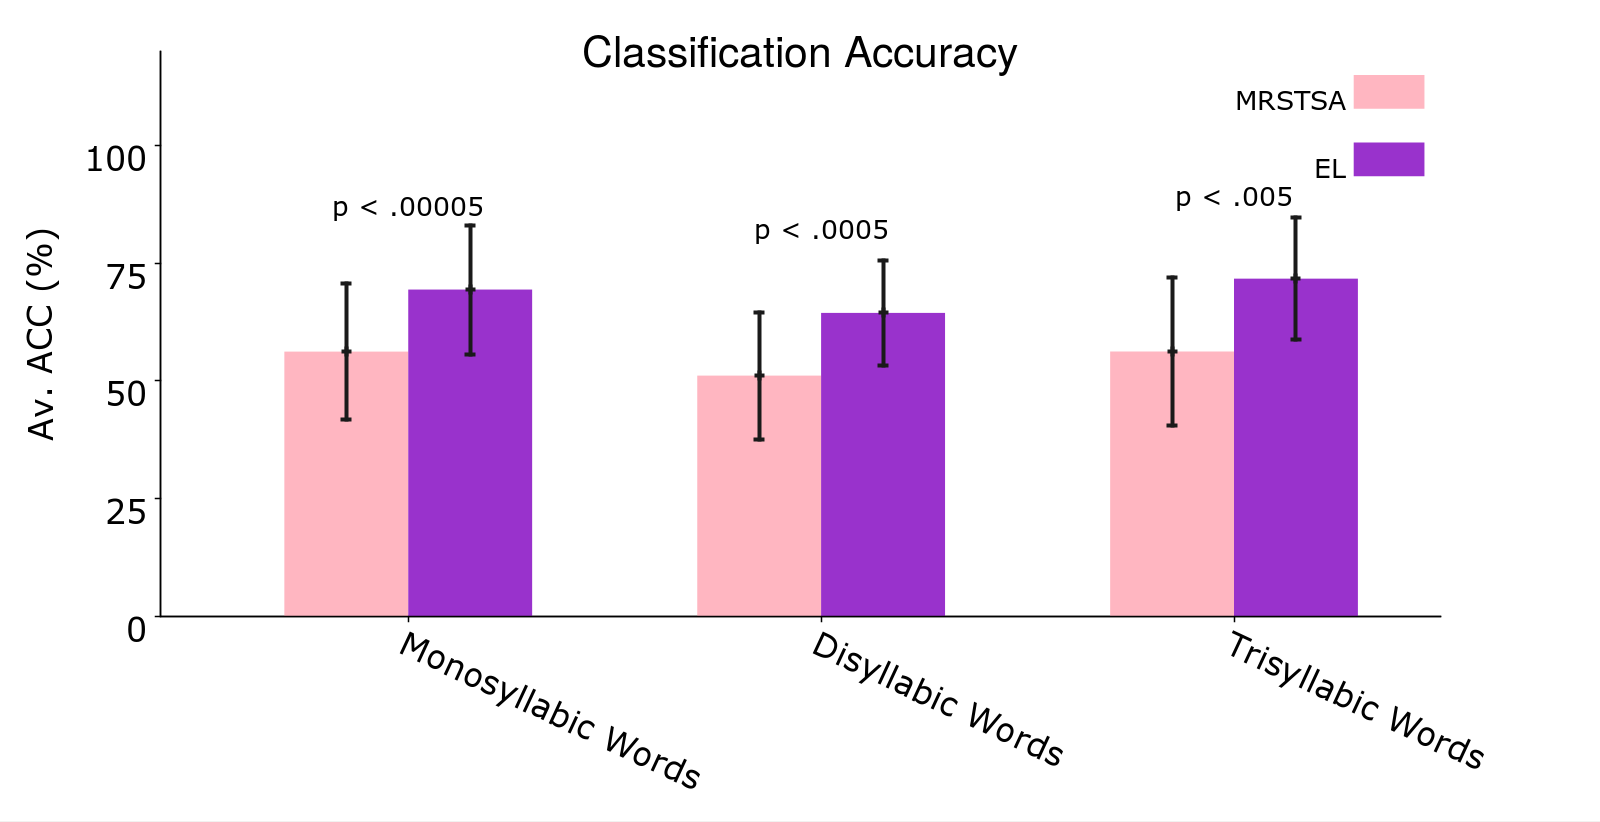
\includegraphics[width=0.8\textwidth]{PLOT1.png}
    \caption{Average Classification Accuracy. Average classification accuracy of grammatically grounded features returned by the \gls{elslc} vs. features returned by the \gls{el} for three experimental conditions. The \emph{p} values correspond to two-tailed paired t-tests (Holm-Bonferroni validated); each for 10 different corpora. Error bars depict 95\% Confidence Interval values. Adapted from https://doi.org/10.1371/journal.pone.0217966 under CC-BY license.}
    \label{fig:PLOT1}
\end{figure}

Once again we performed two-tailed paired t-tests for 10 different corpora from the dataset and applied Holm–Bonferroni corrections with a factor of 3.
As Fig. \ref{fig:PLOT1} shows, the normal \gls{el} performs slightly better than the \gls{elslc}. This global difference in performance is statistically significant for all the experimental conditions according to the t-tests.
A disaggregated statistical analysis showing how distal lateral dendrites contributes to the classification of different syntactic categories is developed in section \ref{Segregated}.
}























\iftoggle{DEBUG}{
\subsection{Análisis Estadísticos Desagregados sobre Categorías Gramaticales Individuales}
\label{Segregated}

Entrenamos dos algoritmos de \gls{svm}, uno recibiendo las salidas de word2vec y el otro recibiendo las salidas desde la \gls{el} para un corpus diferente a los usados en los experimentos previos.
Los resultados del entrenamiento en \gls{svm} con validación cruzada sobre un corpus de 600 oraciones fueron de 83.04\% para word2vec y 91.74\% para la \gls{el}.

Realizamos un análisis estadístico segregado para cada categoría gramatical producida por Enju.
Comparamos el desempeño sobre word2vec vs. la \gls{el} para cada categoría.
A tales fines promediamos el desempeño en cada etiqueta para 10 corpus diferentes--cada uno de 600 oraciones--los cuales estaban compuestos por diferentes oraciones a las utilizadas para entrenar los clasificadores.
Para cada etiqueta computamos los valores \emph{p} correspondientes a pruebas t de dos colas pareadas, cada una para los 10 corpus diferentes.

La Fig. \ref{fig:PLOT3} muestra los resultados para las pruebas comparando word2vec y la \gls{el}.
En la figura mostramos una versión agrupada de las categorías gramaticales producidas por Enju.
Debido a que la frecuencia de ocurrencia de algunas categorías fue de valor despreciable, dichas categorías no fueron incluidas en el análisis.

\begin{figure}[ht!]
    \centering
    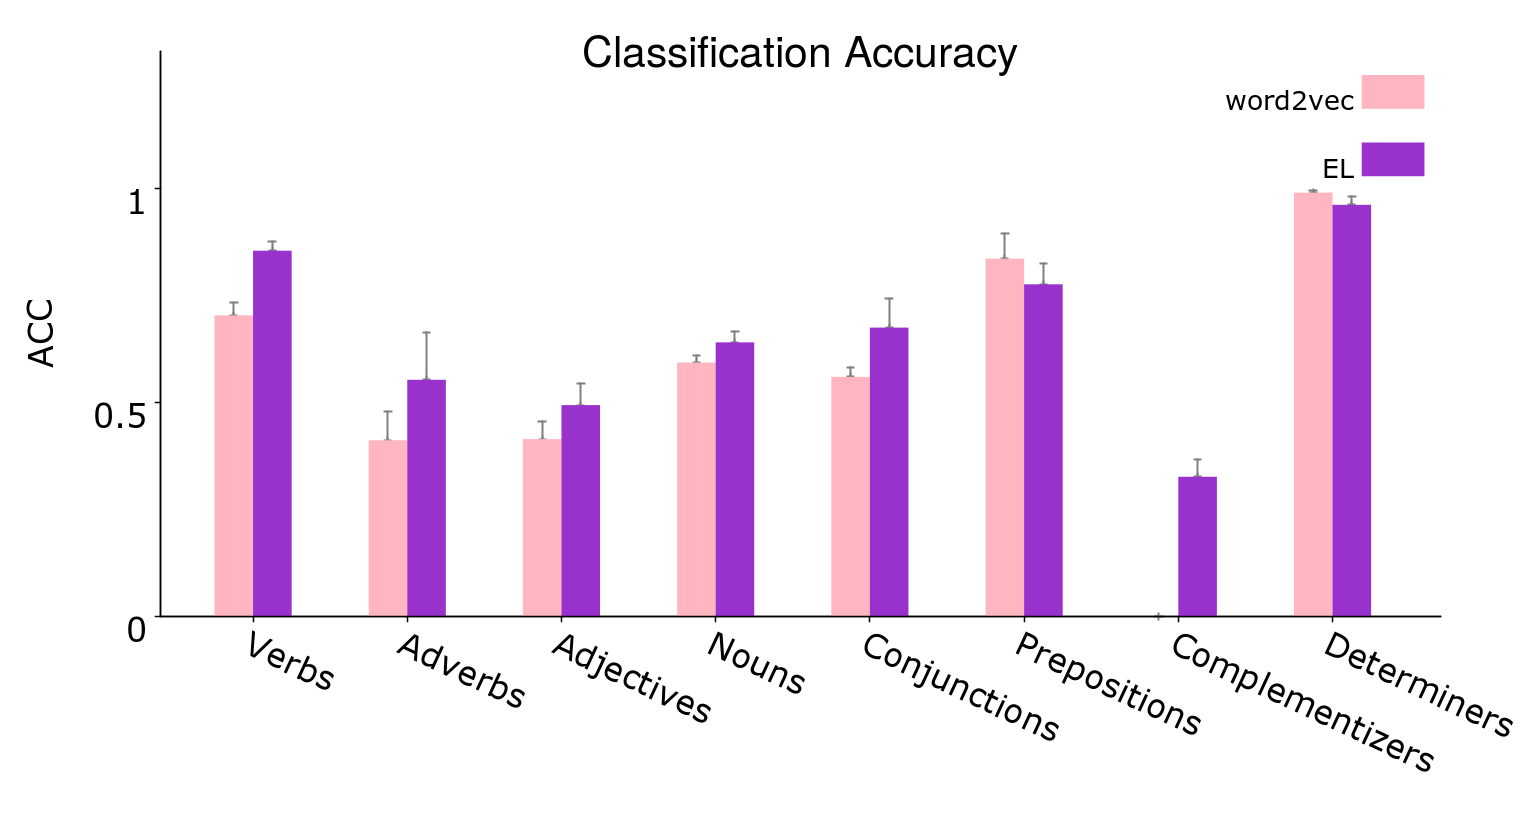
\includegraphics[width=0.99\textwidth]{PLOT3.png}
    \caption{Exactitud Promedio Segregada en Clasificación. Exactitud promedio de clasificación de características gramaticales devueltas por word2vec vs. las características devueltas por la \gls{el} para una versión agrupada de las etiquetas gramaticales. Las barras de error muestran valores de intervalos de confianza del 95\%. Imagen adaptada de https://doi.org/10.1371/journal.pone.0217966 bajo licencia CC-BY.}
    \label{fig:PLOT3}
\end{figure}

La figura muestra una versión desagregada de la evaluación mostrada en la Fig. \ref{fig:PLOT}.
Desde el análisis estadístico, la \gls{el} mejora sobre word2vec significativamente para las etiquetas verbales
\texttt{V\_VBP}, \texttt{V\_VBN}, \texttt{V\_VBD}, \texttt{V\_VBZ}, \texttt{V\_VBG}, y \texttt{V\_VB};
para las etiquetas adverbiales \texttt{ADV\_RB}, \texttt{ADV\_IN} y \texttt{ADV\_RBR};
para las etiquetas de sustantivo \texttt{N\_NN}, \texttt{N\_NNS}, \texttt{N\_FW}, \texttt{N\_PRP}, \texttt{N\_DT} y \texttt{N\_CD};
para los adjetivos \texttt{ADJ\_CD} y \texttt{ADJ\_JJ};
para los complementadores \texttt{C\_TO}  y  \texttt{C\_IN}; para la conjunción de coordinación \texttt{CONJ\_IN} y para la etiqueta preposicional \texttt{P\_IN}.
Por otro lado la \gls{el} obtiene un desempeño menor estadísticamente significativo con respecto a word2vec para la etiqueta determinante
\texttt{D\_PRP\$}; para la conjunción de subordinación \texttt{SC\_IN}; para el adjetivo \texttt{ADJ\_JJS} y para la etiqueta preposicional \texttt{P\_TO}.

Es importante resaltar algunos casos específicos en los que la \gls{el} obtiene un desempeño significativo sin apoyarse en el desempeño de word2vec.
Es decir, en tales casos word2vec tuvo un desempeño del 0\%.
Las categorías gramaticales para las que se da esta situación son por ejemplo los complementadores \texttt{C\_TO} y  \texttt{C\_IN}, las etiquetas adverbiales \texttt{ADV\_IN} y \texttt{ADV\_RBR}, la conjunción de subordinación \texttt{CONJ\_IN} y finalmente los sustantivos \texttt{N\_DT} y \texttt{N\_CD}.


En la Fig. \ref{fig:PLOT4} realizamos el mismo procedimiento desarrollado antes, pero esta vez correspondiente a una versión desagregada de la evaluación mostrada en la Fig. \ref{fig:PLOT2}. En este análisis evaluamos cómo las dendritas laterales distales contribuyen al desempeño en la clasificación de categorías gramaticales individuales.

\begin{figure}[ht!]
    \centering
    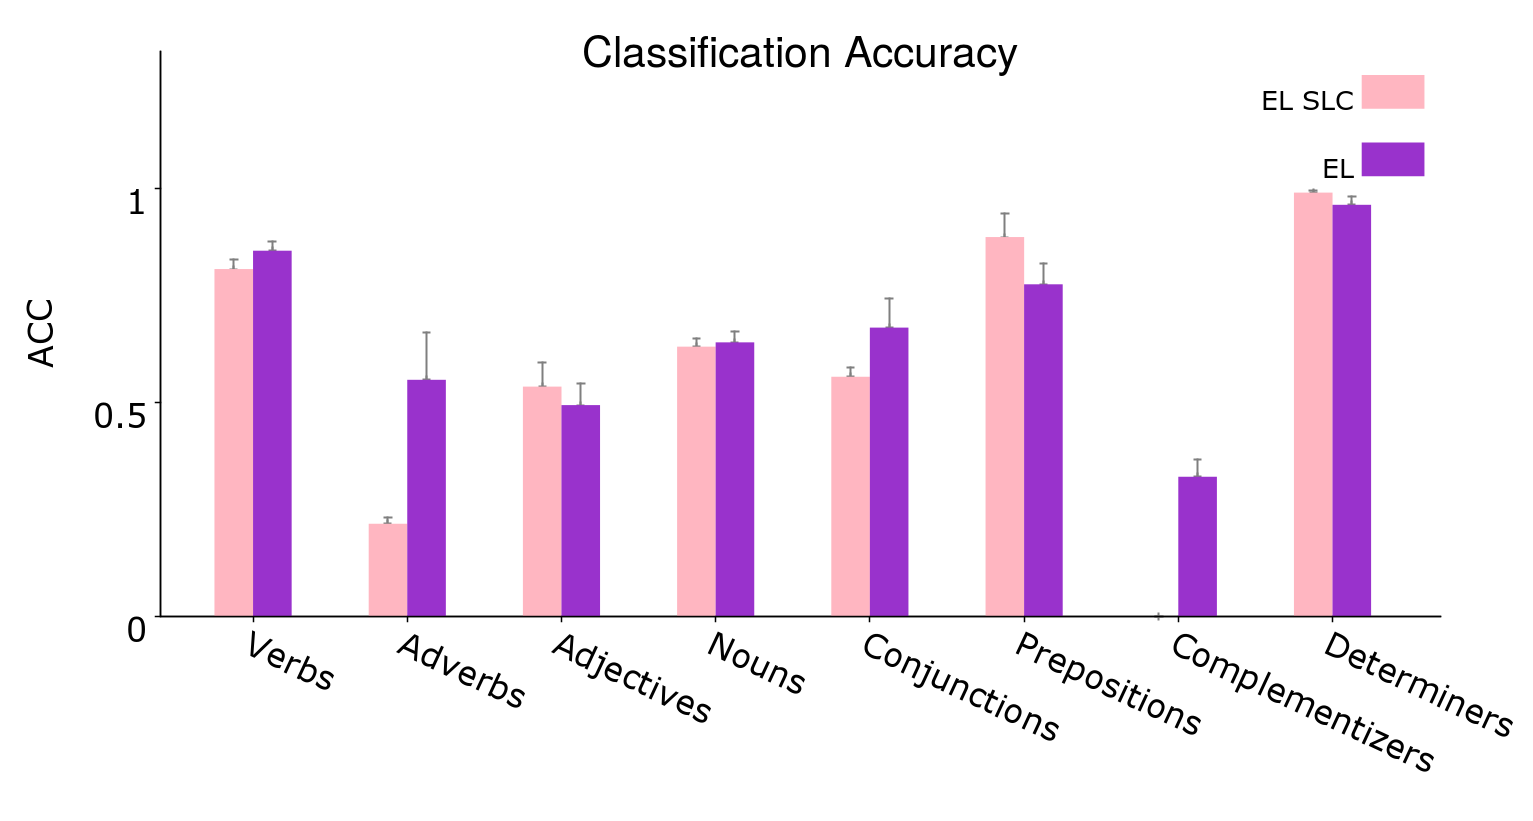
\includegraphics[width=0.99\textwidth]{PLOT4.png}
    \caption{Exactitud Promedio Segregada en Clasificación. Exactitud promedio de clasificación de características gramaticales devueltas por la \gls{elslc} vs. las características devueltas por la \gls{el} para una versión agrupada de las etiquetas gramaticales. Las barras de error muestran valores de intervalos de confianza del 95\%. Imagen adaptada de https://doi.org/10.1371/journal.pone.0217966 bajo licencia CC-BY.}
    \label{fig:PLOT4}
\end{figure}

Desde el análisis estadístico, las dendritas laterales distales producen una mejora significativa de desempeño para las etiquetas verbales
\texttt{V\_VBP}, \texttt{V\_VBD} y \texttt{V\_VB}, para las etiquetas adverbiales \texttt{ADV\_RBS}, \texttt{ADV\_IN}, \texttt{ADV\_RB} y \texttt{ADV\_RBR}, para los complementadores \texttt{C\_IN} y \texttt{C\_TO}, para las etiquetas de sustantivo \texttt{N\_PRP}, \texttt{N\_DT}, y \texttt{N\_CD} y para la conjunción de coordinación \texttt{CONJ\_IN}.
Por otro lado las dendritas laterales distales reducen el desempeño en clasificación para el determinante
\texttt{D\_PRP\$}, para el sustantivo \texttt{N\_NN}, para el adjetivo \texttt{ADJ\_JJR}, para el verbo \texttt{V\_VBZ}, para la conjunción de subordinación \texttt{SC\_IN}, para la partícula \texttt{PRT\_RP} y para la etiqueta preposicional \texttt{P\_TO}.
}{
\subsection{Segregated Statistical Analyses on Individual Grammatical Categories}
\label{Segregated}

We trained two \glspl{svm}--one receiving word2vec outputs and the other receiving the \gls{el} outputs on a different corpus to the corpora used in the previous experiments.
\gls{svm} cross validation training results on the 600-sentences-corpus were 83.04\% on word2vec and 91.74\% on the \gls{el}.

We performed a segregated statistical analysis on each grammatical category produced by Enju.
We compared the performance on word2vec vs. the \gls{el} for each category. To that end we averaged the performance on each tag from 10 different corpora--each of 600 sentences--which were composed by different sentences to the ones used to train the classifiers.
For each tag we computed \emph{p} values corresponding to two-tailed paired t-tests; each for the 10 different corpora.

Fig. \ref{fig:PLOT2} shows the results for the tests comparing word2vec and the \gls{el}.
In the figure we show a clustered version of the grammatical categories produced by Enju.
Since the frequency of occurrence of some categories was of negligible value, they were not included in the analysis.



\begin{figure}[ht!]
    \centering
    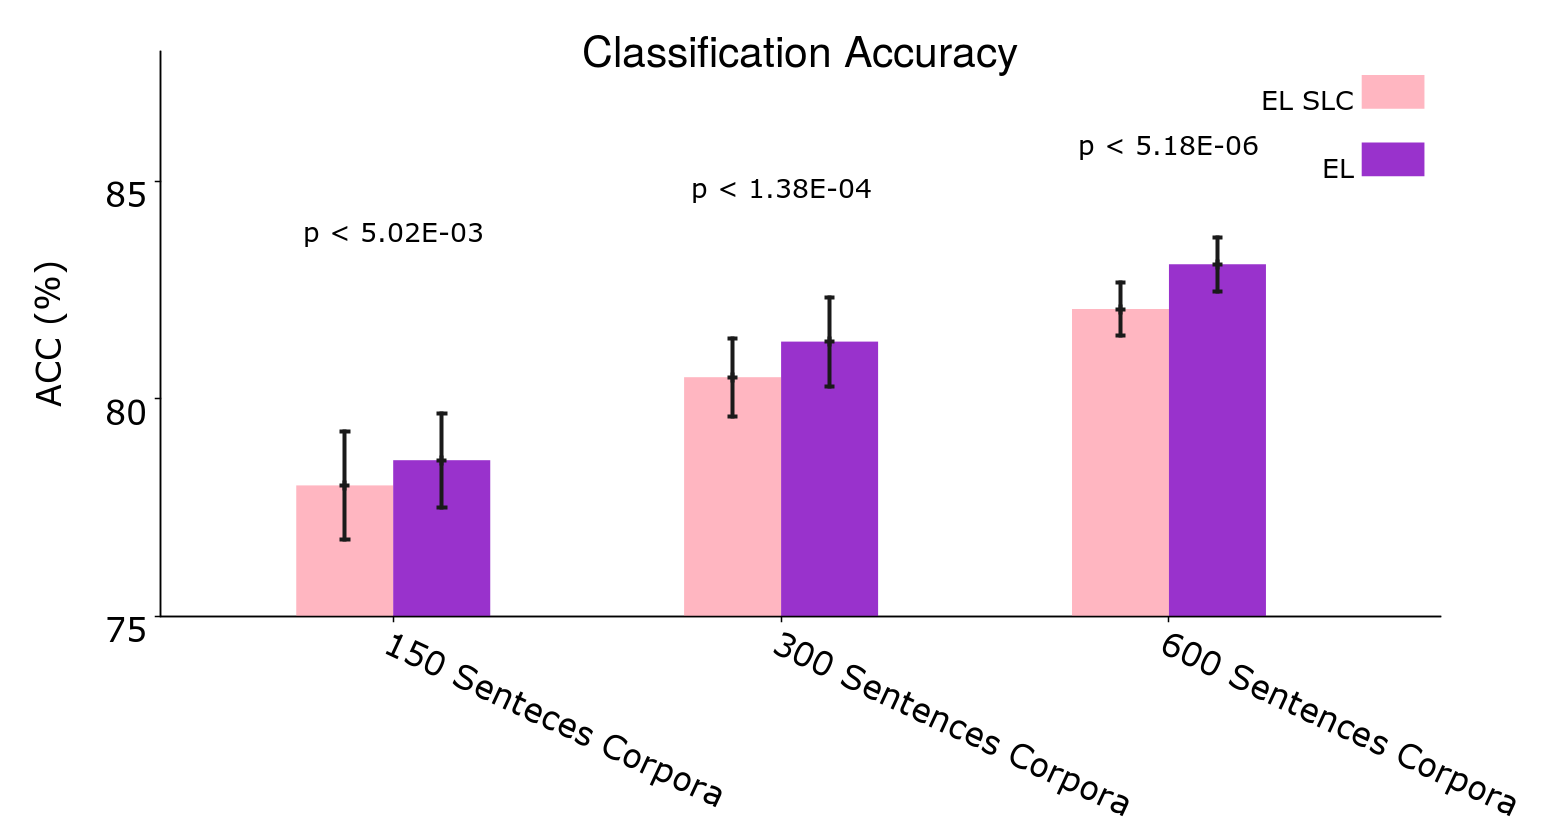
\includegraphics[width=0.99\textwidth]{PLOT2.png}
    \caption{Segregated Average Classification Accuracy. Average classification accuracy of grammatically grounded features returned by word2vec vs. features returned by the \gls{el} for a \emph{coarse-grained} clustered version of the grammatical tags. Error bars depict 95\% Confidence Interval values. Adapted from https://doi.org/10.1371/journal.pone.0217966 under CC-BY license.}
    \label{fig:PLOT2}
\end{figure}

The figure shows a disaggregated version of the evaluation shown in Fig. \ref{fig:PLOT}.
From the statistical analysis, the \gls{el} bootstraps over word2vec significantly for the verbal tags
\texttt{V\_VBP}, \texttt{V\_VBN}, \texttt{V\_VBD}, \texttt{V\_VBZ}, \texttt{V\_VBG}, and \texttt{V\_VB},
for the adverbial tags \texttt{ADV\_RB}, \texttt{ADV\_IN} and \texttt{ADV\_RBR},
for the noun tags \texttt{N\_NN}, \texttt{N\_NNS}, \texttt{N\_FW}, \texttt{N\_PRP}, \texttt{N\_DT} and \texttt{N\_CD},
for the adjectives \texttt{ADJ\_CD} and \texttt{ADJ\_JJ},
for the complementizers \texttt{C\_TO}  and  \texttt{C\_IN}, for the coordination conjunction  \texttt{CONJ\_IN} and for the prepositional tag \texttt{P\_IN}.
On the other hand the \gls{el} gets statistically significant reduced performance respecting word2vec for the determiner tag
\texttt{D\_PRP\$}, for the subordination conjunction \texttt{SC\_IN}, for the adjective \texttt{ADJ\_JJS} and for the prepositional tag \texttt{P\_TO}.

It is important to highlight some specific cases in which the \gls{el} gets significant classification performance without word2vec performance from which to bootstrap. That is, in such cases word2vec had a performance of 0\%. The grammatical categories for which this situation is given are for instance the complementizers \texttt{C\_TO} and  \texttt{C\_IN}, the adverbial tags \texttt{ADV\_IN} and \texttt{ADV\_RBR}, the coordination conjunction  \texttt{CONJ\_IN} and finally the nouns \texttt{N\_DT} and \texttt{N\_CD}.


In Fig. \ref{fig:PLOT3} we conduct the same procedure developed before, but this time corresponding to a disaggregated version of the evaluation shown in Fig. \ref{fig:PLOT1}. In this analysis we evaluate how distal lateral dendrites contribute to the classification performance of individual syntactic categories.

\begin{figure}[ht!]
    \centering
    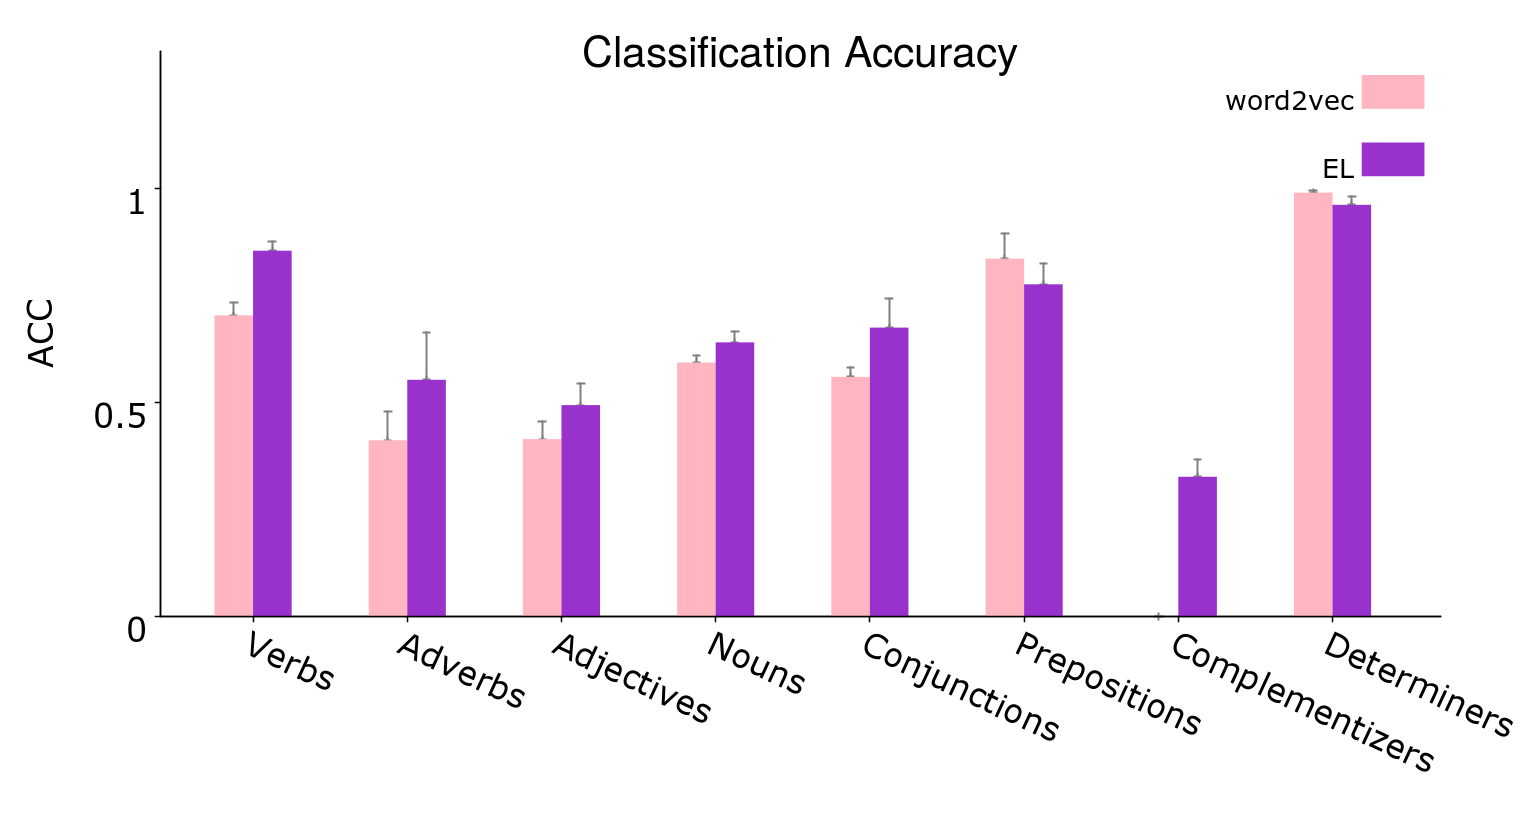
\includegraphics[width=0.99\textwidth]{PLOT3.png}
    \caption{Segregated Average Classification Accuracy. Average classification accuracy of grammatically grounded features returned by the \gls{elslc} vs. features returned by the \gls{el} for a \emph{coarse-grained} clustered version of the grammatical tags. Error bars depict 95\% Confidence Interval values. Adapted from https://doi.org/10.1371/journal.pone.0217966 under CC-BY license.}
    \label{fig:PLOT3}
\end{figure}

From the statistical analysis, distal lateral dendrites produce a significant improvement in performance for the verbal tags
\texttt{V\_VBP}, \texttt{V\_VBD} and \texttt{V\_VB}, for the adverbial tags \texttt{ADV\_RBS}, \texttt{ADV\_IN}, \texttt{ADV\_RB} and \texttt{ADV\_RBR}, for the complementizers  \texttt{C\_IN} and \texttt{C\_TO}, for the noun tags \texttt{N\_PRP}, \texttt{N\_DT}, and \texttt{N\_CD} and for the coordination conjunction \texttt{CONJ\_IN}.
On the other hand, distal lateral dendrites reduce the classification performance for the determiner
\texttt{D\_PRP\$}, for the noun \texttt{N\_NN}, for the adjective \texttt{ADJ\_JJR}, for the verb \texttt{V\_VBZ}, for the subordination conjunction \texttt{SC\_IN}, for the particle \texttt{PRT\_RP} and for the prepositional tag \texttt{P\_TO}.
}






























%\iftoggle{DEBUG}{
%\section{Discusión}

%}{
%\section{Discussion}

%In this paper we introduced a computational model inspired in specific features of brain cortical tissue whose outcome mimics linguistic relevant selection mechanisms found in brain cortex~\cite{Gibson1998-GIBCOS, Hagoort2005OnBB, Rego1993TheCB, 10.1371/journal.pone.0177794}.

%By means of the experimental results presented here we show how the convergence of linguistic constraints from different sources, improves the classification of grammatical functions carried by constituents within a sentence context.

%For instance, when analyzing a specific sentence, both algorithms lose number sense in the first word (\texttt{wolves}). Except for such case, the \gls{el} catches the number sense in the rest of the cases in which plural nouns appear (\texttt{ungulates} and \texttt{feeders}), while word2vec continues losing number sense in those examples too.
%As can be seen in Fig. \ref{fig:PLOT2} and from the statistical analysis conducted in section \ref{Segregated}, the \gls{el} significantly outperforms word2vec in the classification of singular and plural nouns.

%In our implementation, coarse-grained word category constraints from apical dendrites do not provide enough information to the \gls{el} to make such distinction. Initially our group contemplated the possibility that syntactic constraints coming from lateral dendritic activation within the sequence of constituents, could fulfil the information needed by the \gls{el} to constraint the choices among different unification options. In such way, the \gls{el}, engaging such constraints, could have ended up activating only the most suitable option given the information received.
%In this example, \glsfirst{ds} information from word2vec does not suffice to distinguish the number attribute in nouns, but the incorporation of syntactic constraints such as the adjectives preceding nouns could have biased the probability towards the plural attribute. Furthermore, larger distance dependencies such as the word \texttt{are} in the phrase \texttt{are opportunistic feeders}, could have influenced the classification given the sequential properties incorporated in the \gls{el} \cite{Cui:2016:COS:3030654.3030660}.
%Since syntactic constraints do not appear in the first word of the sentence, the \gls{el} could have made the same kind of mistake than word2vec, and neither \glspl{ds} nor coarse-grained word category constraints would provided sufficient information as to catch the plural attribute in the noun.

%In order to test such hypothesis, in section \ref{slc} our group tested a version of the \gls{el} without lateral dendritic arms.
%Fig. \ref{fig:PLOT1} shows that lateral dendrites in our model play certain role in the integration of sequential information
%given the statistical significance returned by the experiments.
%Yet, a disaggregated analysis of Fig. \ref{fig:PLOT1}--conducted in section \ref{Segregated}--allowed us to conclude that the improvement in the distintion between singular and plural nouns comes from the combination of afferent and apical constraints, and not from the sequential information provided by lateral constraints.
%This phenomenon can be seen in section \ref{Segregated}, in which the performance in the classification of singular nouns is reduced with the incorporation of lateral dendritic trees while the performance on the classification of plural nouns is not significantly affected.


%The classification of verbs in the sentence (\texttt{feed} and \texttt{eat}), clearly shows the importance of the coarse-grained word category constraints from apical dendrites \cite{shi_newborn_1999,shi_morgan_allopenna_1998,Shi1995PerceptualCO,lohmann_phonological_2017,doi:10.1207/s15327078in1002_5}. In such regard, word2vec confers a very high weight to nouns in both examples, completely misclassifying the word \texttt{feed} as a singular noun and giving almost the same probability (33.9\% vs. 33.3\%) to the tags verb in base form and singular noun when the verb \texttt{eat} appears. The \gls{el} on the other hand, virtually disregards the classification of such verbs as nouns, misclassifying \texttt{feed} as a verb in base form although providing a high chance to the correct tag (the second highest). The \gls{el} also produces a correct classification of \texttt{eat}, providing a high probability to the correct tag.

%In section \ref{Segregated}, Fig. \ref{fig:PLOT2} shows that grammatical constructions for verbs are classified significantly better by the \gls{el}. The unique exception is for the case of modal verbs (\texttt{V\_MD}) as can be inferred from the statistical analysis.
%From Fig. \ref{fig:PLOT3}, we can see that lateral dendrites contribute significantly to the classification of verbs.
%From the statistical analysis specific improvements are for the \emph{verb, non-3rd person singular present} (\texttt{V\_VBP}), \emph{verb, past tense } (\texttt{V\_VBD}) and \emph{verb, base form} (\texttt{V\_VB}).

%Adjectives are quite remarkable as can be seen in Fig. \ref{fig:Sentence1}. Even though the adjectives \texttt{sized} and \texttt{available} are correctly classified by both algorithms, there is a notorious difference in such classifications which can be appreciated in the soundness with which the \gls{el} attributes chances to the correct tag in both cases. On the other hand, word2vec is  indeterminate, attributing a very low chance to the correct tag, especially in the case of \texttt{sized}, in which the algorithm attributes almost the same probability to the tags adjective, verb in past participle and singular noun. Another important example is given with the word \texttt{medium}. Even when the appearance of such word counts as a success for word2vec, the reality is that the \gls{el} produces a correct classification of it as an adjective, and such classification is sound due to the high probability assigned to the tag. From Fig. \ref{fig:PLOT2}, we can see that the \gls{el} improves the classification of adjectives significantly. Fig. \ref{fig:PLOT3} shows that this improvement does not come from the contribution provided by distal lateral dendrites.

%It is important to highlight some specific cases for which the \gls{el} builds its own classification performance from a word2vec performance of 0\%. 
%The most prominent cases are for the following tags:
%\texttt{C\_TO}, with typical examples like \emph{... the voice \textbf{to} renew ...} or \emph{... released \textbf{to} radio ...} and
%\texttt{CONJ\_IN}, with typical examples like \emph{... as well \textbf{as} ...} or \emph{... rather \textbf{than} ...}.
%Moreover, the classification performance in such cases is completely sustained by distal lateral dendrites as can be inferred from the statistical analysis conducted in section \ref{Segregated}.

%For some adverbs, such as
%\emph{superlative} (\texttt{ADV\_RBS}) with examples like \emph{the third \textbf{most} common ...} or \emph{his \textbf{most} serious poem ...}, \emph{subordinating conjunction} (\texttt{ADV\_IN}) with examples like \emph{after wandering \textbf{around} he discover ...} or \emph{... soon \textbf{after}} and \emph{adverb, comparative} (\texttt{ADV\_RBR}) with examples like \emph{... to \textbf{better} measure future cash flow} or \emph{... her autobiography \textbf{more} important than her poetry}, the \gls{el} classification performance is fully sustained by distal lateral dendrites.

%Adverbs (\texttt{ADV\_RB}) with examples like \emph{... that is \textbf{almost} completely black} or \emph{it was released \textbf{only} in australia}; are classified significantly better by the \gls{el} and distal lateral dendrites--even when not exclusively--contribute significantly to such classification performance.

%Compared to word2vec, the \gls{el} activates fewer phrasal configurations, narrowing down the spectrum of alternative binding candidates. It assigns higher probability values to fewer tags and generally such tags are the correct ones or closer to the correct ones. This fact is supported by the higher hit rate of the \gls{el} compared to word2vec (Fig. \ref{fig:PLOT}).



%Regarding related works in the field, \cite{WENNEKERS200616} introduced a modeling approach in which multiple area networks are built of anatomically identical features. Similarly to the model we present in this paper, the architecture of such network introduces cells which include feedforward, feedback and lateral connections which are set up by means of associative principles motivated by Hebb’s rules \cite{doi:10.1002/1097-4679(195007)6:3<307::AID-JCLP2270060338>3.0.CO;2-K}.
%In a more recent work, using the same modelling principles \cite{TOMASELLO2017111} developed a physiologically plausible artificial neural-network that replicated sensorimotor, multimodal and language areas. The experiments reported emergent \emph{semantic circuits} for object- and action-related words which exhibited category-specificity in modality-preferential areas.
%Even though results from both works can be compared with real experimental data--thanks to the realistic neurocomputational facet of the models--the experimental profiles were mainly centered on statistical correlation measurements and over semantic aspects--not grammar was involved in the work. 
%The learning of syntactic structure was not in the scope of such research. In general \cite{WENNEKERS200616} manifested the acquisition of syntactic structure as a difficult problem in assembly networks. Furthermore, no \gls{ml} like recognition tasks were conducted, the corpora used for the experiments were artificially generated and the models were not tested on classification invariance.

%A computational model that assigns thematic roles to sentence constituents has been previously developed by \cite{STJOHN1990217}. The model disambiguates words, instantiates vague words, and elaborates implied roles. Recently, this computational approach was used to explain the N400 event-related brain potential presenting a computationally explicit account for the emerging representation of sentence meaning \cite{rabovsky_modelling_2018}. The model succeeded capturing diverse empirical neural responses, showing that essential aspects of human language processing can be effectively represented by a proper connectionist approach.
%Nevertheless, the model lacked a mapping of neurophysiological characteristics in cortical dynamics and used optimization algorithms (i.e. backpropagation) which are difficult to map in neural tissue.

%\cite{Dominey2009NeuralNP} on the other hand, incorporated the functional neurophysiology of sentence comprehension (along with non-linguistic sequence processing), in a neural network model whose architecture was constrained by \gls{cstc} neuroanatomical connectivity and functional imaging data. The model was able to learn and perform several types of language and artificial syntax tasks. Their approach includes the interaction among several \glspl{ba} involved in language processing--such as \gls{ba} 47, 45 and 44/6 in the \gls{lifg}. Nonetheless, such model is also forced to choose the correct options through supervised error-driven learning methods. Such methodology, assumes the existence of internal \emph{teaching signals} in the brain. Teaching signals are needed to force the output layer to the correct answer, enabling the network to backpropagate the errors.

%\cite{michalon_meaning-driven_2019} developed an explicit algorithmic implementation of a parallel processing architecture that explains how syntactic and semantic information processing can interact selectively during language comprehension. The architecture advances towards the organization of language in the brain focusing in the articulation between syntax and semantics and the essence of prediction in language comprehension. The work is clearly inspired by the psychology and neuroscience of language, but it does not incorporate biologically accurate features of neural computation in its implementation.

%In the present work the computational model developed, is inspired in the biology of the mammalian neocortex and simulates cortical tissue incorporating columnar organization, spontaneous micro-columnar formation, \glspl{sdr} and adaptation to contextual activation. In addition, different roles to proximal and distal dendritic configurations simulating pyramidal cells are assigned. We incorporate important physiological and anatomical phenomena, such as the consideration of dendritic branches as active and independent processing elements, the stochastic activation of brain cells and \glspl{mfe} originated by prediction failures in the network manifesting as the activation of many neurons in a \gls{cc} impairing \glspl{sdr} formation--among others. Most \glspl{ann}, such as those used in previous works \cite{STJOHN1990217, rabovsky_modelling_2018, Dominey2009NeuralNP, michalon_meaning-driven_2019}, use artificial neurons without considering active dendrites and with an unrealistic low number of synapses, thus missing fundamental functional properties present in the brain. Furthermore, unlike established computational models, the model presented here does not incorporate optimization methods such as those found in supervised or reinforced algorithms. Even though influential research lines underpin the idea of \emph{credit assignment} supporting backpropagation processes in cortex \cite{10.7554/eLife.22901}, so far there is not enough evidence to justify the inclusion of such complex process in the brain. Moreover, our concerns regarding backpropagation in brain tissue go beyond the complexity of its algorithmic implementation. These implementations require the existence of teaching signals. Although there is evidence that animals can represent desired behavioral outputs with internal goal representations \cite{gadagkar_dopamine_2016}, it is unknown whether teaching signals indeed exist in the brain.
%On the other hand, although very new and compelling algorithmic approaches such as BERT \cite{DBLP:journals/corr/abs-1810-04805} and GPT-2 \cite{radford_language_nodate, DBLP:journals/corr/VaswaniSPUJGKP17} are making far-reaching changes in \gls{nlp} in general, they continue needing complex optimization algorithms of difficult justification in brain cortex. Furthermore, they apply \emph{Attention} mechanism without restriction demanding the full availability of all words in input sentences without providing clear explanations of memory mechanisms to sustain such phenomena in brain.

%In the present work, we replace \emph{teaching signals} used in other systems--specially needed by backpropagation-like optimization--by the uniform and simple correlation of \glspl{sdr} activation coming from different cortical patches. Our hypothesis is that when noise is impairing the smooth individualization of a pattern coming from one source, the brain correlates such information with information coming from other sources in which the noise has not been too detrimental for the pattern that the subject seeks to classify.
%In the present model, when \glsfirst{ds} information from afferent dendrites is not sufficient for grammatical disambiguation of a sentence constituent, coarse-grained word category information from apical dendrites helps in such disambiguation. In the case that coarse-grained word category clues cannot compensate the lack of \gls{ds} information, syntactical constraints from lateral dendrites finally come in handy. Functional connectivity across different cortical areas has been shown to facilitate speech comprehension when the intelligibility of the speech signal is reduced~\cite{Obleser2283}.

%On the other hand, the presence of reciprocal connectivity between different areas as well as recurrent connectivity inside the same area is a repeated pattern in cortex. The lack of reciprocal and/or recurrent anatomical connectivity among some cortical areas in our simulations lies in the current implementation of our model. Since \glspl{ds} are provided by word2vec we are neither able to inject backward signals from the \gls{el} nor able to implement recurrent connectivity inside such standalone model. In the case of coarse-grained word categories, their static \glspl{sdr} are neither able to be enriched by recurrent connectivity nor by backward connections from the \gls{el} module.

%In this research we use some features of the information processing gradient discovered in the \gls{lifg} as a guidance to explain a plausible interaction of different lexical constraints in cortex. In this complex region of the neocortex information coming from \glspl{ba} 47 and 45 is involved in semantic processing \cite{GOUCHA2015294, DECARLI2007933, PMID:15528098, NEWMAN201051} and we use it as the \gls{ds} input gateway to the \gls{el}.
%It is important to highlight though that there are alternative pathways--beyond \gls{ba} 47--in which semantic information is processed
%such as the temporal and inferior parietal lobes--among others \cite{Binder2011TheNO}.

%In fact, many other sources of information--which turn out to be useful for early infant language acquisition--have not been yet considered in our computational approach. For instance, it has been shown that iconic gestures boost speech comprehension under adverse listening conditions \cite{HOLLE2010875}. Neurocognitive studies of motor representations of speech sounds, action-related language, sign language and co-speech gestures are also tightly coupled to the language system \cite{Willems2007NeuralEF}.
%Future work in the model will be directed towards integrating information from more sources than the ones presently used.
%We will also enrich coarse-grained word category information from apical dendrites with direct phonological cues to procure a more holistic linguistic integration.
%With this implementation we will also be able to apply backward connectivity possibly derived from \glspl{ba} 45/44 to \gls{ba} 6 and also to include recurrence in specific stages of the model related to coarse-grained syntax and phonology.
%Finally, for future developments of this work, we will add reinforced mechanisms to the model, including neuromodulator-like effects in the algorithm which could significantly enhance performance.
%}
























%\iftoggle{DEBUG}{
%}{
%\subsection{Conclusion}

%This research brings a novel explanation on how cortical activation for linguistic constraints could produce grammatical discrimination emergence in sentence constituents from the interaction of specific areas in the human brain. These areas present a linguistic processing gradient which is precisely mapped in the cortical dynamics of a computational approach which simulates particular characteristics evaluated as suitable for linguistic computations in human neocortex.
%We introduce a biologically plausible computational model which incorporates specific features from the mammalian cortex. Our model utilizes Hebbian-like rules without involving optimization mechanisms extensively used in prevalent \glsfirst{ml} algorithms, but of difficult justification in cortical tissue.
%We use such model to explain unification operations at semantic and syntactic levels of language on the cortical \glsfirst{lifg}.
%We show how cortical \glsfirst{sdr} activation features returned by our model are well suited to attain classification of lexical grammatical functions of words bootstrapping \glsfirst{ds} features returned by word2vec.
%We evaluate this research as valuable for future and more brain-inspired \gls{ml} applications of \gls{nlp} as well as a complementary validation for psycho-linguistic theories of language processing. 
%}






